
%!TEX root = ../template.tex
%%%%%%%%%%%%%%%%%%%%%%%%%%%%%%%%%%%%%%%%%%%%%%%%%%%%%%%%%%%%%%%%%%%%
%% chapter8.tex
%% NOVA thesis document file
%%
%% Chapter with lots of dummy text
%%%%%%%%%%%%%%%%%%%%%%%%%%%%%%%%%%%%%%%%%%%%%%%%%%%%%%%%%%%%%%%%%%%%

\typeout{NT FILE chapter8.tex}%

\chapter{Experimental Analysis, Validation and Discussion}
\label{cha:results}

The previous chapters (Chapters \ref{cha:text_} and \ref{cha:segmentation}) introduced the methods developed in this thesis. For each topic, a few examples were presented to help understand and follow the explanation and description of the proposed methods. In this chapter, we go further into testing and validating the algorithms to provide evidence that these are relevant and contribute to the state-of-the-art in the time series data mining field. The performance was evaluated on public datasets, introduced in Chapter \ref{cha:data}.
\par
Considering the diversity of methods developed, this chapter will be divided into each contribution following the topics presented in the previous Chapters:

\begin{itemize}
\item \textbf{Information Retrieval with the \gls{ssm}}:
We presented three main applications of retrieving information from the \gls{ssm}, namely for novelty segmentation, periodic segmentation and similarity association. The process for novelty segmentation was validated in public datasets and its performance compared with two referenced methods ($WL$ - window based segmentation, and $BS$ - binary segmentation). In addition, we applied this strategy in a change point detection benchmark, where we were able to compare its performance with all methods available in the benchmark. We show an application example for periodic segmentation and query-based segmentation in one public dataset, and results are computed based on ground-truth annotations.

\item \textbf{Pattern Search with \gls{ssts}}:
In this topic, we provide use-cases where \gls{ssts} is used to retrieve specific patterns. Each step of the proposed method are highlighted. Specific metrics (see Section \ref{subsec:complex}) are used to compare the \gls{ssts} query used with a standard python-based implementation for the search problem.

\item \textbf{Time Series Classification with \gls{hearts}}:
Having demonstrated the possibility of using \gls{ssts} to search for patterns, we explore its usage to extract a textual representation of time series and apply text-mining methods to perform the classification. A public benchmark was used to perform this analysis and \gls{hearts} was compared with the 1-NN \gls{ed}. We also provide evidence in several use-cases of how the weights of the \gls{tfidf} model can be used to highlight the most relevant areas of the signal, contributing to the interpretability of results.

\item \textbf{Pattern Search with \gls{quots}}:
The second proposed method for pattern search in time series will be evaluated with several use-cases. We also evaluate its ability to separate classes of hand gestures with simple queries. Finally, we also show an example of \textit{pupetteering} as a toy problem, and as a possible application of this method. 
\end{itemize}

\section{Information Retrieval with the Self-Similarity Matrix}

\subsection{Novelty Segmentation}

In this section, we present several examples of how the novelty function (recall Section \ref{sec:novelty_search}, retrieved from the \gls{ssm}, is useful for the segmentation of time series. We also provide a measure of the algorithm's performance considering ground truth events from public benchmarks, while also comparing our proposed solution with existing methods for change point detection from the \textit{Turing Change Point Detection Benchmark} \cite{cpd_alan}.

\subsubsection{Quantiative Evaluation Metrics}

In order to evaluate the performance of our proposed method in general scenarios, we applied the algorithm to Datasets 3, 4, 5, 6, 7 and 12 (\textit{HAR1}, \textit{WISDM}, \textit{EMG}, \textit{ECG1}, \textit{ECG2}, and \textit{ENABL3S}, see Sections \ref{dat:dataset3}, \ref{dat:dataset5},\ref{dat:dataset6},\ref{dat:dataset7}, \ref{dat:dataset8} and \ref{dat:dataset13}). The evaluation was divided into \textit{biosignals-related applications}, and the general change point detection benchmark (Dataset 9 - \textit{ATCPD}, see Section \ref{dat:dataset10}). The biosignals experiments are associated with public datasets from Physionet, the \textit{UCI Machine Learning Repository} and the \textit{UCR Semantic Segmentation Benchmark}, involving different contexts (\gls{har}, hand posture, and noise detection) and sensor types (\gls{acc}, \gls{gyro}, \gls{emg}, \gls{abp} and \gls{ecg}).

The quantitative evaluation on biosignals' public datasets was made by accumulating true positive ($TP$), false positive ($FP$), and false negative ($FN$) values with a tolerance zone around the ground truth events. The applied reasonable tolerance was the ground truth wrapped by a window size of the \gls{ssm} computation, inside which a detected event was counted as a $TP$. The case that no estimated event was found inside the tolerance band was considered an $FN$. An estimated event outside the tolerance or duplicating to an already counted $TP$ were regarded as an $FP$. The F1-score based on the precision and recall values was calculated from $TP$, $FN$, and $FP$ values (recall definitions and equations from Section \ref{subsec:event_metrics}).

An online repository \footnote{\url{https://github.com/JmdRodrigues/PhDThesis/tree/main/ProjectCode/NOVA/Results/Tables}} is also available where Tables with detailed parameter usage are presented, namely the window sizes, kernel sizes, and thresholds. In addition, the distribution of F1-scores is available in Appendix \ref{appendix:tables_detailed} Section \ref{app_sec:detailed_results}. 


\subsubsection{Biosignals' Segmentation}

In the evaluation of biosignal segmentation, the performance of our proposed method was compared with existing approaches available on the Python library \textit{ruptures}, namely the window-based segmentation ($WL$) and the binary segmentation ($BS$) \cite{review_2}. For these methods, we used the \textit{normal} cost function, which accounts for mean and variance changes. The benchmark evaluation referred to the best score obtained from the state-of-the-art methods available on repository  \cite{cpd_alan}. The evaluation procedure to detect $TP$, $FP$ and $FN$ was the one followed on \cite{cpd_alan}.

The method has been computed in the same conditions and followed the same procedure for all datasets' records. The features used were the same for each record (see Appendix 2 - \ref{appendix:tables_detailed}), varying the timescale parameter, the overlap size of the sliding window, and the kernel size. The peak detection strategy based on a threshold mechanism is the same for all records, while the threshold value varies from record to record. Results for publicly available datasets are listed in Tables \ref{tab:biosignals_results} and \ref{tab:biosignals_results2}, and Table \ref{tab:alanturing} expands the performance by F1-scores in detecting the change point events from a benchmark.

\begin{table}[H]
    \centering
    \caption{Overall results for the performance of the method on novelty segmentation, including true positives (TP), false positives (FP) and false negatives (FN), precision (P), recall (R) and F1-score (F1) values. The last row provides the macro averaged F1-scores (\textit{M.A. F1}) of the four datasets.}
    \label{tab:biosignals_results}
    \resizebox{\textwidth}{!}{%
    \begin{tabular}{crrrrrrrrrrrrrrrrrr}
\toprule
          & \multicolumn{6}{c}{Novelty} & \multicolumn{6}{c}{WL} & \multicolumn{6}{c}{BS}\\
\midrule
  Dataset &     TP &   FP &   FN &    P &    R &   F1 &     TP &    FP &    FN &    P &    R &   F1 &    TP &    FP &    FN &    P &    R &   F1\\
\cmidrule(lr){1-1} \cmidrule(lr){2-7} \cmidrule(lr){8-13} \cmidrule(lr){14-19}
HAR1 &  166 &  16 &  13 &  0.91 &  0.93 &  0.92 &  169 &    9 &   10 &  0.95 &  0.94 &  0.95 &  125 &   58 &   54 &  0.68 &  0.70 &  0.69 \\
WISDM &   784 &   87.0 &   92 &  0.90 &  0.89 &  0.90 &   709 &  140.0 &  167 &  0.84 &  0.81 &  0.82 &   657 &   255.0 &   219 &  0.72 &  0.75 &  0.73 \\
ECG1 &   18 &    1.0 &    0 &  0.95 &  1.00 &  0.97 &    13 &    5.0 &    5 &  0.72 &  0.72 &  0.72 &    16 &     2.0 &     2 &  0.89 &  0.89 &  0.89 \\
ECG2 &  155 &    9.0 &   13 &  0.95 &  0.92 &  0.93 &   139 &   13.0 &   29 &  0.91 &  0.83 &  0.87 &   122 &    58.0 &    46 &  0.68 &  0.73 &  0.70 \\
EMG &  695 &  68 &  33 &  0.91 &  0.95 &  0.93 &  608 &  123 &  120 &  0.83 &  0.84 &  0.83 &  351 &  413 &  377 &  0.46 &  0.48 &  0.47 \\
Enabl3s &  3433 &  469.0 &  366 &  0.88 &  0.90 &  0.89 &  2941 &  327.0 &  858 &  0.90 &  0.77 &  0.83 &  2618 &  1322.0 &  1181 &  0.66 &  0.69 &  0.68 \\
\midrule
M.A. F1 & - & - & - & - & - & 0.91 &-&-&-&-&- & 0.83 &-&-&-&-&-& 0.69\\
\bottomrule
\end{tabular}}
\end{table}


\begin{table}[H]
    \centering
    \caption{Results to summarize the comparison between the methods tested. In this table, each record of each dataset is counted for each method as a win, draw or loss. The count is made for each dataset and finally, for all datasets altogether (W|D|L).}
    \label{tab:biosignals_results2}
    \resizebox{\textwidth}{!}{%
    \begin{tabular}{crrrrrrrrr}
\toprule
          & \multicolumn{3}{c}{Novelty} & \multicolumn{3}{c}{WL} & \multicolumn{3}{c}{BS}\\
\midrule
  Dataset &     Wins &   Draws &   Loses & Wins &   Draws &   Loses & Wins &   Draws &   Loses\\
\cmidrule(lr){1-1} \cmidrule(lr){2-4} \cmidrule(lr){5-7} \cmidrule(lr){8-10}
HAR1 &  0 &  0 &  2 &  2 &  0 &  0 &  0 & 0 & 2\\
WISDM &  42 &  1 &  8 &  5 &  1 &  45 &  3 & 0 & 48\\
ECG1 &   2 &   7 &   0 &  0 &  4 &  5 & 0 & 6 & 3\\
ECG2 &  10 &  1 &  1 &  0 &  0 &  12 &   1 &   1 & 10 \\
EMG &  31 &  2 &  3 &  3 &  2 &  31 &  0 &  0 &  36 \\
Enabl3s &  320 & 52 & 104 & 100 & 47 & 329 & 3 & 7 & 466\\
\midrule
Overall W|D|L & 5 & 0 & 1 & 1 & 0 & 5 & 0 & 0 & 6\\
\bottomrule
\end{tabular}}
\end{table}

The illustrative examples provided in Section \ref{sec:use_cases_ssm} corroborate the proposed method's capability in segmenting real, complex, and multimodal biosignals datasets. As Tables \ref{tab:biosignals_results} and \ref{tab:biosignals_results2} convey, an overall macro-averaged 0.91 F1-score is achieved, while the competitors' overall F1-scores are 0.83 ($WL$), and 0.69 ($BS$), respectively, with the proposed method winning in 5 of the 6 datasets in the overall F1-score ranking.

For Datasets 3, 4, 5 and 12 (HAR1, WISDM, EMG and Enabl3s, see Sections \ref{dat:dataset3}, \ref{dat:dataset5}, \ref{dat:dataset6} and \ref{dat:dataset13}), the window-based methods, \textit{novelty} and $WL$, performed much better than the $BS$ method, mainly because the sliding window algorithm with a full set of features comprehensively characterizes changes in the signal.
The standard $WL$ uses cost functions searching for mean/variance value changes in the signal, which achieves a high F1-score in most of the datasets explored, even identifying transitions between dynamic activities, such as \textit{Walking}/\textit{Upstairs}.
Our proposed method had a similar performance with a worse count in $FP$ values, where the added features did not improve the segmentation performance.
In contrast, our proposed method, complemented by additional features, had a much better performance than the $WL$ method in Datasets 4, 5 and 6 (WISDM, EMG and Enabl3s, see Sections \ref{dat:dataset5}, \ref{dat:dataset6} and \ref{dat:dataset13}), having a higher F1-score in a total of 35(/45), 31(/34) and 320(/423) records for each corresponding dataset.
Adding features enabled a more robust and sensitive detection of pattern changes, although it missed some changes between similar patterns, like \textit{Walking} and \textit{Upstairs/Downstairs} in Dataset 3 (HAR1, see Section \ref{dat:dataset3}), which are the primary source of the $FN$ value.
Similar to the $FN$ values, the $FP$ values of our proposed method are mostly superior to other methods. It nonetheless leaves room for discussion. Some events are not marked as changes in specific activities, but the signal pattern actually changes. For example, Figure \ref{fig:use_case1}(bottom) exposes pattern changes during an \textit{Upstairs}/\textit{Downstairs} activity unlabelled in the ground truth, possibly due to a flight of stairs. The novelty function is sensitive to such pattern changes, which inevitably contributes to the $FP$ values during the comparison with the ground truth. The higher count in $FP$ might also be caused by the peak search strategy. Being based on a simple threshold, it might detect more peaks that are not relevant, which makes the $P$ comparable to the \textit{WL} method. Another strategy should be considered for this step.

For Dataset 6 and 7 (ECG2 and ECG1, see Sections \ref{dat:dataset7} and \ref{dat:dataset8}) the proposed method was also superior. Although \gls{ecg}-based jump artefact detection is fundamental, the $WL$ method could not find all the segmentation borders, while the $BS$ method worked better. In Dataset 6 (ECG2, see Section \ref{dat:dataset7}), the same \gls{ecg} signal was noised with different \gls{snr} levels to form a new set of resultant signals. Overall, our proposed method was able to detect the changes between noisy segments and clean segments with noise down to 12 dB. At 6 dB, the proposed method achieved an F1-score of 0.67 with references of 0.64 ($WL$), and 0.34 ($BS$).

\subsubsection{Segmentation Benchmark}

In order to compare the proposed method with other state-of-the-art approaches, we used a benchmark provided by the Alan Turing Institute \cite{cpd_alan} (Dataset 9, ATCPD, see Section \ref{dat:dataset10}). The performance was evaluated by change point event detection in each time series available, summarized in Figure \ref{fig:cdd_alant}, where each referenced method applied its best score in the benchmark (see Tables \ref{tab:alanturing} and \ref{tab:params_results_alanT}).

\begin{table}
    \caption{Comparison of the F1-scores between our proposed method (\textit{novelty}) and other algorithms' benchmarks in Dataset 9 (see Section \ref{dat:dataset10}). The calculation of all one-dimensional signals' average performance and all signal's average performance does not include columns with a gray background where no change point should be detected, or a signal error was present. Bold values represent the best F1-score for this specific dataset.
    T: timed out; F: failed compiling.}
    \label{tab:alanturing}
    \resizebox{\textwidth}{!}{
    \begin{tabular}{l|c|cccccccccccccc}
     \toprule
    Dataset & \textsc{novelty} & \textsc{amoc} & \textsc{binseg} & \textsc{bocpd} & \textsc{bocpdms} & \textsc{cpnp} & \textsc{ecp} & \textsc{kcpa} & \textsc{pelt} & \textsc{prophet} & \textsc{rbocpdms} & \textsc{rfpop} & \textsc{segneigh} & \textsc{wbs} & \textsc{zero}\\
    \midrule
    \multicolumn{16}{l}{\textbf{One-dimensional}} \\
    \midrule
      \cellcolor{gray!100}bank & \cellcolor{gray!100}0 & \cellcolor{gray!100}\textbf{1.000} & \cellcolor{gray!100}\textbf{1.000} & \cellcolor{gray!100}\textbf{1.000} & \cellcolor{gray!100}0.500 & \cellcolor{gray!100}0.054 & \cellcolor{gray!100}0.200 & \cellcolor{gray!100}0.333 & \cellcolor{gray!100}0.400 & \cellcolor{gray!100}\textbf{1.000} & \cellcolor{gray!100}T & \cellcolor{gray!100}0.015 & \cellcolor{gray!100}\textbf{1.000} & \cellcolor{gray!100}0.043 & \cellcolor{gray!100}\textbf{1.000}\\
    bitcoin & 0.694 & 0.507 & 0.690 & 0.733 & 0.533 & 0.611 & 0.625 & 0.665 & \textbf{0.735} & 0.446 & T & 0.284 & \textbf{0.735} & 0.690 & 0.450\\
    brent\_spot & \textbf{0.861} & 0.465 & 0.670 & 0.609 & 0.239 & 0.607 & 0.636 & 0.553 & 0.586 & 0.249 & T & 0.521 & 0.586 & 0.564 & 0.315\\
    businv & \textbf{0.927} & 0.588 & 0.588 & 0.588 & 0.455 & 0.386 & 0.370 & 0.294 & 0.490 & 0.275 & 0.370 & 0.261 & 0.588 & 0.289 & 0.588\\
    centralia & 0.984 & 0.909 & \textbf{1.000} & \textbf{1.000} & \textbf{1.000} & \textbf{1.000} & 0.909 & \textbf{1.000} & \textbf{1.000} & 0.763 & 0.846 & \textbf{1.000} & \textbf{1.000} & 0.556 & 0.763\\
    children\_per\_woman & \textbf{0.879} & 0.678 & 0.663 & 0.712 & 0.405 & 0.344 & 0.551 & 0.525 & 0.637 & 0.310 & 0.504 & 0.246 & 0.637 & 0.500 & 0.507\\
    
    co2\_canada & 0.851 & 0.544 & 0.856 & \textbf{0.924} & 0.479 & 0.642 & 0.875 & 0.867 & 0.670 & 0.482 & 0.542 & 0.569 & 0.872 & 0.681 & 0.361\\
    
    construction & \textbf{0.933} & 0.696 & 0.709 & 0.709 & 0.410 & 0.602 & 0.709 & 0.634 & 0.709 & 0.324 & 0.340 & 0.185 & 0.709 & 0.523 & 0.696\\
    
    debt\_ireland & 0.974 & 0.760 & \textbf{1.000} & \textbf{1.000} & 0.892 & 0.958 & 0.980 & \textbf{1.000} & \textbf{1.000} & 0.469 & 0.748 & 0.824 & \textbf{1.000} & 0.538 & 0.469\\
    
    gdp\_argentina & \textbf{0.968} & 0.889 & 0.947 & 0.947 & 0.583 & 0.818 & 0.889 & 0.800 & 0.947 & 0.615 & 0.452 & 0.615 & 0.947 & 0.421 & 0.824\\
    
    gdp\_croatia & \textbf{1.000} & \textbf{1.000} & 0.824 & \textbf{1.000} & 0.583 & \textbf{1.000} & 0.824 & 0.583 & 0.824 & 0.824 & 0.824 & 0.400 & 0.824 & 0.167 & 0.824\\
    
    gdp\_iran & \textbf{0.921} & 0.696 & 0.652 & 0.862 & 0.492 & 0.620 & 0.824 & 0.734 & 0.808 & 0.652 & 0.737 & 0.636 & 0.808 & 0.576 & 0.652\\
    
    gdp\_japan & \textbf{1.000} & \textbf{1.000} & 0.889 & \textbf{1.000} & 0.615 & 0.667 & \textbf{1.000} & 0.500 & 0.889 & 0.889 & 0.889 & 0.222 & 0.889 & 0.222 & 0.889\\
    
    global\_co2 & 0.625 & \textbf{0.929} & \textbf{0.929} & 0.889 & 0.458 & 0.667 & \textbf{0.929} & 0.667 & \textbf{0.929} & 0.463 & 0.547 & 0.293 & \textbf{0.929} & 0.250 & 0.846\\
    
    homeruns & \textbf{0.933} & 0.812 & 0.829 & 0.829 & 0.650 & 0.650 & 0.829 & 0.829 & 0.812 & 0.723 & 0.397 & 0.661 & 0.812 & 0.664 & 0.659\\
    
    iceland\_tourism & 0.652 & 0.947 & 0.947 & 0.947 & 0.486 & 0.391 & \textbf{1.000} & 0.486 & 0.643 & 0.220 & 0.667 & 0.200 & 0.947 & 0.200 & 0.947\\
    
    jfk\_passengers & \textbf{0.978} & 0.776 & 0.776 & 0.776 & 0.650 & 0.602 & 0.651 & 0.437 & 0.776 & 0.354 & T & 0.491 & 0.776 & 0.437 & 0.723\\
    
    lga\_passengers & 0.885 & 0.561 & 0.620 & 0.704 & 0.563 & 0.606 & \textbf{0.892} & 0.526 & 0.537 & 0.366 & T & 0.592 & 0.537 & 0.674 & 0.535\\
    
    \cellcolor{gray!100}measles & \cellcolor{gray!100}0 & \cellcolor{gray!100}\textbf{0.947} & \cellcolor{gray!100}\textbf{0.947} & \cellcolor{gray!100}\textbf{0.947} & \cellcolor{gray!100}0.486 & \cellcolor{gray!100}0.118 & \cellcolor{gray!100}0.080 & \cellcolor{gray!100}0.281 & \cellcolor{gray!100}0.153 & \cellcolor{gray!100}0.391 & \cellcolor{gray!100}F/T & \cellcolor{gray!100}0.030 & \cellcolor{gray!100}\textbf{0.947} & \cellcolor{gray!100}0.041 & \cellcolor{gray!100}\textbf{0.947}\\
    
    
    nile & \textbf{1.000} & \textbf{1.000} & \textbf{1.000} & \textbf{1.000} & 0.800 & \textbf{1.000} & \textbf{1.000} & 0.824 & \textbf{1.000} & 0.824 & 0.667 & \textbf{1.000} & \textbf{1.000} & \textbf{1.000} & 0.824\\
    
    ozone & 0.857 & 0.776 & 0.723 & 0.857 & 0.778 & 0.750 & \textbf{1.000} & 0.667 & \textbf{1.000} & 0.723 & 0.651 & 0.429 & \textbf{1.000} & 0.286 & 0.723\\
    
    quality\_control\_1 & \textbf{1.000} & \textbf{1.000} & \textbf{1.000} & \textbf{1.000} & 0.667 & 0.667 & \textbf{1.000} & 0.667 & \textbf{1.000} & 0.500 & 0.286 & 0.667 & \textbf{1.000} & 0.667 & 0.667\\
    
    quality\_control\_2 & \textbf{1.000} & \textbf{1.000} & \textbf{1.000} & \textbf{1.000} & 0.667 & \textbf{1.000} & \textbf{1.000} & \textbf{1.000} & \textbf{1.000} & 0.750 & .429 & \textbf{1.000} & \textbf{1.000} & \textbf{1.000} & 0.750\\
    
    quality\_control\_3 & \textbf{1.000} & \textbf{1.000} & \textbf{1.000} & \textbf{1.000} & 0.766 & 0.571 & \textbf{1.000} & \textbf{1.000} & \textbf{1.000} & 0.667 & T & 0.800 & \textbf{1.000} & \textbf{1.000} & 0.667\\
    
    quality\_control\_4 & \textbf{0.974} & 0.810 & 0.873 & 0.787 & 0.561 & 0.658 & 0.726 & 0.658 & 0.780 & 0.780 & T & 0.241 & 0.780 & 0.608 & 0.780\\
    
    \cellcolor{gray!100}quality\_control\_5 & \cellcolor{gray!100}0 & \cellcolor{gray!100}\textbf{1.000} & \cellcolor{gray!100}\textbf{1.000} & \cellcolor{gray!100}\textbf{1.000} & \cellcolor{gray!100}0.500 & \cellcolor{gray!100}\textbf{1.000} & \cellcolor{gray!100}\textbf{1.000} & \cellcolor{gray!100}\textbf{1.000} & \cellcolor{gray!100}\textbf{1.000} & \cellcolor{gray!100}\textbf{1.000} & \cellcolor{gray!100}0.500 & \cellcolor{gray!100}\textbf{1.000} & \cellcolor{gray!100}\textbf{1.000} & \cellcolor{gray!100}\textbf{1.000} & \cellcolor{gray!100}\textbf{1.000}\\
    
    rail\_lines & 0.909 & 0.846 & 0.846 & \textbf{0.966} & 0.889 & \textbf{0.966} & \textbf{0.966} & 0.800 & 0.846 & 0.537 & 0.730 & 0.615 & 0.889 & 0.205 & 0.537\\
    
    ratner\_stock & 0.933 & 0.776 & 0.824 & 0.868 & 0.559 & 0.396 & 0.776 & 0.754 & 0.824 & 0.280 & T & 0.203 & 0.824 & 0.378 & 0.571\\
    
    robocalls & \textbf{0.979} & 0.800 & 0.966 & 0.966 & 0.750 & 0.862 & 0.966 & 0.966 & 0.966 & 0.636 & 0.846 & 0.714 & 0.966 & 0.714 & 0.636\\
    
    scanline\_126007 & 0.887 & 0.710 & 0.920 & \textbf{0.921} & 0.829 & 0.906 & 0.870 & 0.838 & 0.889 & 0.644 & T & 0.649 & 0.889 & 0.818 & 0.644\\
    
    scanline\_42049 & \textbf{0.977} & 0.485 & 0.879 & 0.962 & 0.889 & 0.713 & 0.910 & 0.908 & 0.910 & 0.269 & T & 0.460 & 0.910 & 0.650 & 0.276\\
    
    seatbelts & 0.659 & 0.824 & \textbf{0.838} & 0.683 & 0.583 & 0.735 & 0.683 & 0.621 & 0.683 & 0.452 & 0.383 & 0.563 & 0.735 & 0.583 & 0.621\\
    
    shanghai\_license & \textbf{0.979} & 0.966 & 0.868 & 0.868 & 0.605 & 0.600 & 0.868 & 0.465 & 0.868 & 0.532 & 0.389 & 0.357 & 0.868 & 0.385 & 0.636\\
    
    \cellcolor{gray!100}uk\_coal\_employment & \cellcolor{gray!100}F & \cellcolor{gray!100}F & \cellcolor{gray!100}F & \cellcolor{gray!100}F & \cellcolor{gray!100}0.617 & \cellcolor{gray!100}F & \cellcolor{gray!100}0.513 & \cellcolor{gray!100}0.513 & \cellcolor{gray!100}F & \cellcolor{gray!100}\textbf{0.639} & \cellcolor{gray!100}F & \cellcolor{gray!100}F & \cellcolor{gray!100}F & \cellcolor{gray!100}F & \cellcolor{gray!100}0.513\\
    
    unemployment\_nl & 0.820 & 0.742 & \textbf{0.889} & 0.876 & 0.592 & 0.747 & 0.755 & 0.744 & 0.788 & 0.566 & F/T & 0.628 & 0.788 & 0.801 & 0.566\\
    
    us\_population & 0.636 & \textbf{1.000} & 0.889 & \textbf{1.000} & 0.615 & 0.232 & 0.471 & 0.276 & 0.500 & 0.159 & T & 0.889 & 0.889 & 0.113 & 0.889\\
    
    usd\_isk & \textbf{0.914} & 0.785 & 0.704 & 0.785 & 0.678 & 0.674 & 0.785 & 0.601 & 0.657 & 0.489 & 0.510 & 0.462 & 0.678 & 0.636 & 0.489\\
    
    well\_log & 0.814 & 0.336 & 0.914 & 0.832 & 0.743 & 0.822 & \textbf{0.928} & 0.776 & 0.873 & 0.149 & T & 0.923 & 0.873 & 0.832 & 0.237\\
    
    \midrule

    \textbf{Average F1-measure (1D)} & \textbf{0.845} & 0.739 & 0.798 & 0.822 & 0.596 & 0.651 & 0.784 & 0.657 & 0.766 & 0.482 & 0.354 & 0.517 & 0.797 & 0.517 & 0.599\\
    
    \midrule

    \multicolumn{16}{l}{\textbf{Multidimensional}} \\

    \midrule
    
    apple & \textbf{0.949} &  &  & 0.916 & 0.445 &  & 0.745 & 0.634 &  &  & F/T &  &  &  & 0.594\\
    
    bee\_waggle\_6 & 0.657 &  &  & \textbf{0.929} & 0.481 &  & 0.233 & 0.634 &  &  & 0.245 &  &  &  & \textbf{0.929}\\
    
    occupancy & \textbf{0.953} &  &  & 0.919 & 0.735 &  & 0.932 & 0.812 &  &  & F/T &  &  &  & 0.341\\
    
    run\_log & 0.994 &  &  & \textbf{1.000} & 0.469 &  & 0.990 & 0.909 &  &  & 0.380 &  &  &  & 0.446\\
    
    \midrule

    \textbf{Average F1-measure (ALL)} & \textbf{0.871} & n.a. & n.a. & 0.855 & 0.604 & n.a. & 0.797 & 0.683 & n.a. & n.a. & 0.343 & n.a. & n.a. & n.a. & 0.61\\

    \midrule
    
	\textbf{WINS (ALL)} & 16 & 0 & 2 & 2 & 0 & 0 & 3 & 0 & 0 & 0 & 0 & 0 & 0 & 0 & 0\\
    
    \textbf{DRAWS (ALL)} & 6 & 9 & 8 & 11 & 1 & 6 & 8 & 4 & 9 & 1 & 0 & 3 & 8 & 2 & 0\\
    \textbf{LOSES (ALL)} & 12 & 25 & 24 & 21 & 33 & 28 & 23 & 30 & 25 & 33 & 34 & 31 & 26 & 32 & 34\\
    \bottomrule
    \end{tabular}}
\end{table}

\begin{figure}
    \centering
    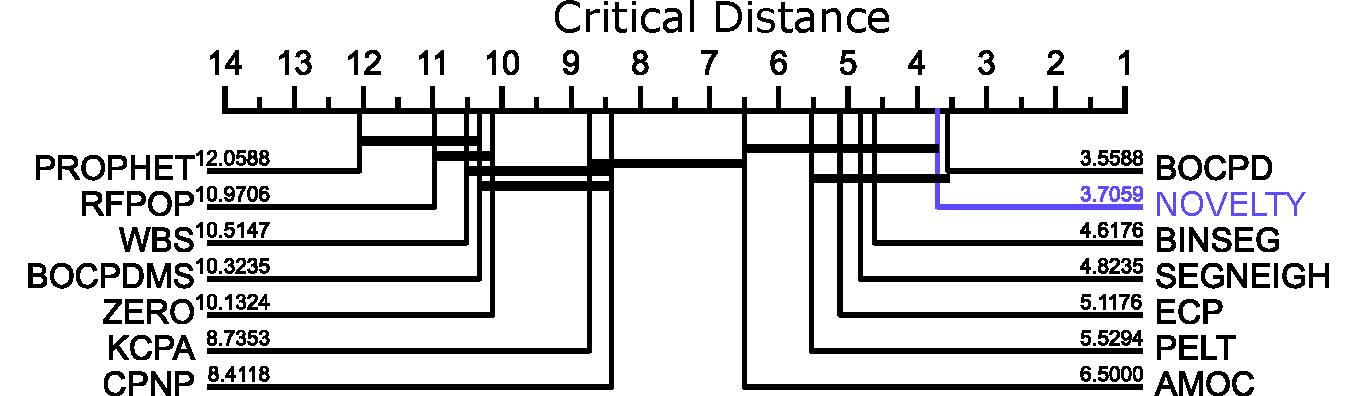
\includegraphics[width=\linewidth]{critical_distance_novelty.pdf}
    \caption{Critical distance diagram comparing the methods used in \cite{cpd_alan} (except \textit{RBOCPDMS}) and the \textit{novelty function} on Dataset 9 (see Section \ref{dat:dataset10}). The performance measure corresponds to the F1-score for all single-dimension datasets of the benchmark, except for the ones identified in Table \ref{tab:alanturing} with a gray background. A thick horizontal line groups a set of classifiers that are not significantly different in the statistical test \cite{critical_dif}.}
    \label{fig:cdd_alant}
\end{figure}

As unfolded in Figure \ref{fig:cdd_alant}, the critical distance diagram ranks the proposed method second, suggesting no significant difference in performance among methods that only work in uni-dimensional datasets. The global average F1 measure of the proposed method is 0.87 for both uni and multidimensional datasets, with a higher F1-score than all other methods in 16 of the 34 datasets. In contrast, the \textit{BOCPD} method had an overall of 2 wins against all other methods. 
The two null scores are because no change point was supposed to be found in the corresponding time series. The results obtained in this benchmark restate that our proposed method is promising, having a performance that competes with several state-of-the-art methods in the problem of novelty segmentation. It should be stressed that the proposed method applies to multidimensional time series, while two of the best-ranked methods in Figure \ref{fig:cdd_alant} do not. In addition, the proposed method retrieves not solely segmentation points but also higher-level information as periodic changes and cross-segment similarity measures, which is an advantage over the \textit{BOCPD}.

\subsubsection{Time Complexity}
\label{sec:time_complexity}

In terms of computation time, the algorithm performs (1) a sliding window to extract features, which is \textit{O(n)} complexity and (2) performs the dot product between matrices, which is traditionally \textit{O($m^2n$)} (recall that \textit{r} is the number of features and \textit{n} is the size of the inputted signal). Finally, the correlation of a kernel on the \gls{ssm}'s diagonal has a complexity of $O(nM^2)$ (recall that $M=2L+1$, being the size of the sliding kernel).

%Rewrite
The sliding window to extract features has an $O(n)$ time complexity. The dot product between matrices has a conventional $O(m^2n)$ time complexity. Expressly, $m$ and $n$ represent the number of features and the inputted signal's size, respectively, in our proposed method. The correlation computation of a kernel on the \gls{ssm}'s diagonal has a complexity of $O(nM^2)$, where the sliding kernel's size $M$ equals $2L+1$.

\subsubsection{Discussion of Novelty Segmentation Results}
\label{sec:novelty_seg_discussion}

Several parameters affect the detection results of desired patterns, especially the window size, the overlap percentage, and the kernel size, which influence visual outputs and the novelty function. These parameters can be explained with the analogy of a camera:

\begin{itemize}
    \item The window size works like the \textit{zoom function}, defining the scale of interest in the time series. Larger windows, corresponding to lower \textit{zoom values}, allow the similarity calculation of longer \textit{subsequences}, while smaller windows, serving like a \textit{zoom-in} function, search for local details and unobtrusive changes.
    \item The overlap percentage, working as a down-sampler of the time series, is the \textit{camera sensor}, which determines the image's pixel resolution. A full resolution of the \gls{ssm} is only achieved with total overlap, and the lower the overlap percentage, the less accurate are the highlighted changes.
    \item The sliding kernel's size concerns the novelty function's sharpness of the detected changes. The larger it is, the smoother the output function will be. Potentially, the kernel size can be scaled to the window size, even with a slight accuracy decrease.
\end{itemize}

With enough computational resources available, the overlap percentage can be maximized so that the \gls{ssm} can mirror the full details. Admittedly, such an operation is not necessary for many real applications, but reduces the variables to facilitate other parameters' tuning experiments, which is one of our subsequent research topics.
The computational resource, i.e., the memory bandwidth and the calculation time (see Section \ref{sec:time_complexity}) is a limitation in this current stage, since the \gls{ssm} increases exponentially with the increase in the time series size. We ascertained that downsampling the time series with a lower overlap percentage is a valid option, advanced by a hierarchical search strategy for addressing the memory limitation, as exemplified in the walking-series instance in Section \ref{sec:acc_har}. Another potential efficiency-enhancing solution is to only compute the \gls{ssm}'s central diagonal with the kernel size corresponding to the interest areas of segmentation borders, which obtains efficiency gains in exchange for the sacrifice of periodicity and similarity measures between \textit{subsequences}.

A reasonable intuition based on the understanding of signal characteristics should help configure the parameters mentioned above that are fundamental for computing the \gls{ssm} and the novelty function, as Figure \ref{fig:intuition} demonstrates a starter example for segmentation purposes. The upper part of Figure \ref{fig:intuition} draws different \gls{ssm}s on the same \gls{ecg} record (A) from Dataset 2 (ECG1, see Section \ref{dat:ecg1}) computed with sequentially larger window lengths from 0.01 to 2 seconds.
The appropriate window length depends on the purpose of the search:

\begin{itemize}
    \item If a small window length, e.g., 0.05 seconds, is chosen, the novelty function will mostly detail changes within a heartbeat.
    \item If opting for a window length approximately equal to the \gls{ecg}'s \textit{PQRS} complex, each transition between complexes will be projected.
    \item If even larger windows are applied, e.g., 1 or 2 seconds, the jump artefact will be more significant on the \gls{ssm} and be spotlighted on the novelty function. Hence, in such a case, the window length of 1 second should be appropriate for segmenting clean versus noisy ECG signals.
\end{itemize}

\begin{figure}
    \centering
    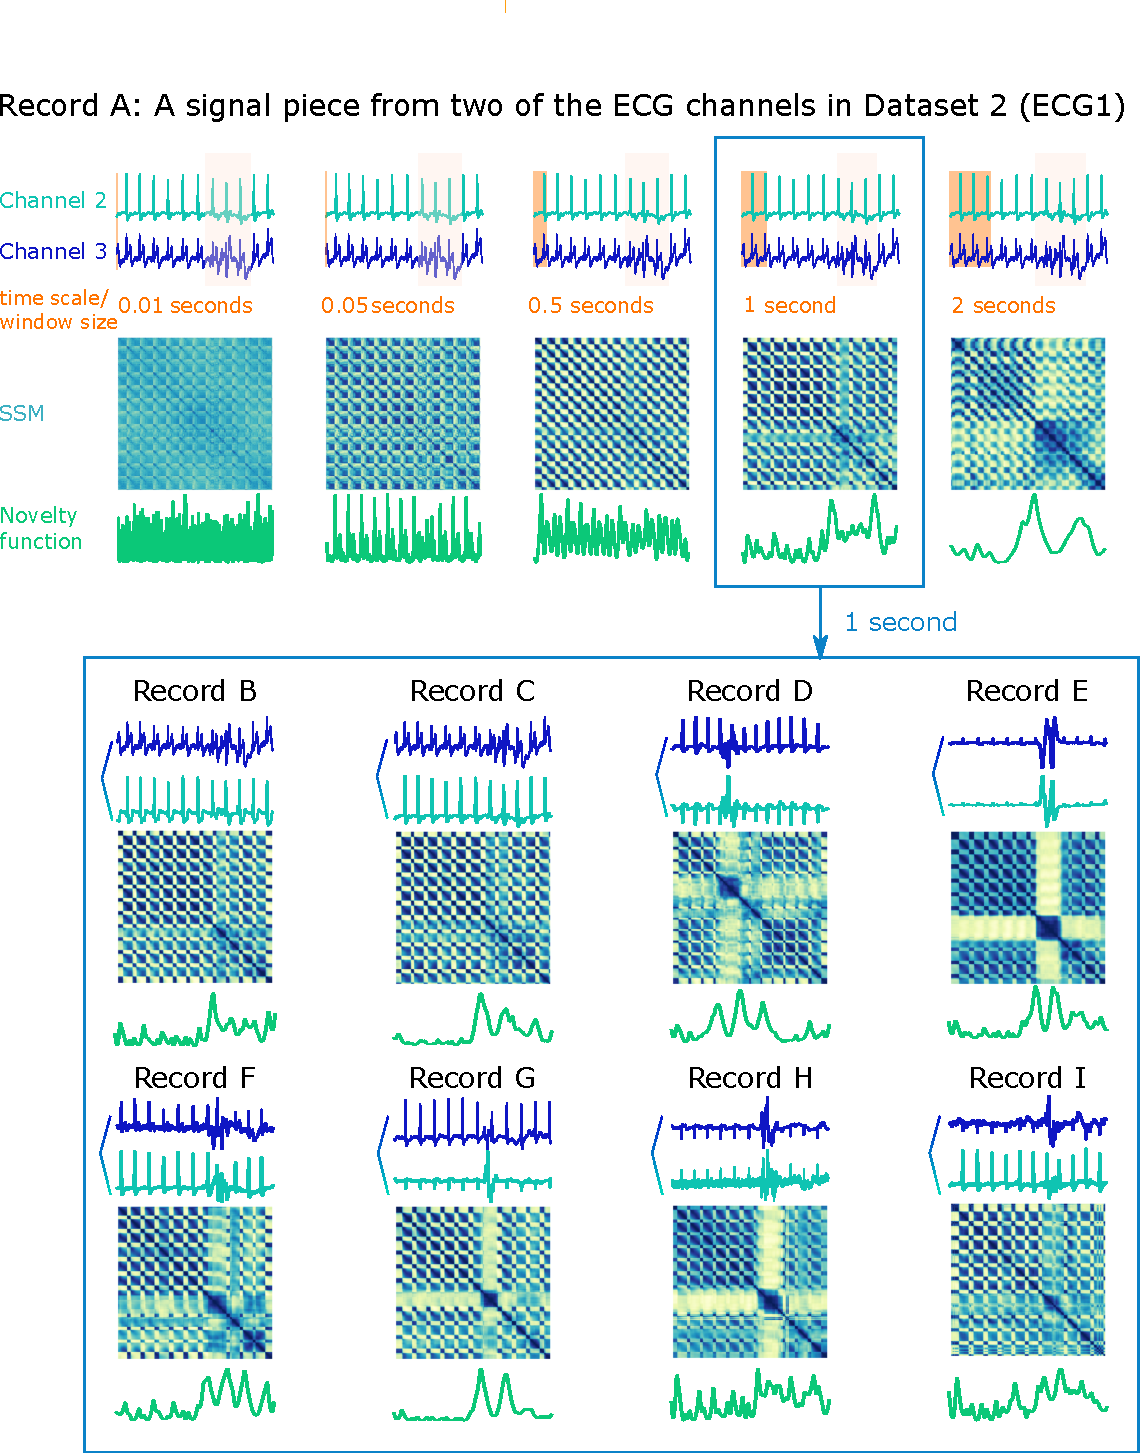
\includegraphics[width=\linewidth]{explaining_changes_in_time_scale.pdf}
    \caption{Illustrative example of window length intuition on records of Dataset 6 (ECG1, see Section \ref{dat:dataset7}). Top: different \gls{ssm}s on the same \gls{ecg} record A computed with sequentially larger window lengths from 0.01 to 2 seconds. The novelty functions are calculated with a kernel size equal to the window size and an overlap of 95\%. Bottom: The 1-second window length is further applied as an example to indicate that parameters turned in the representation experiments can be generalized to all other records of the same dataset (B-I) to compute their corresponding \gls{ssm} representations and novelty functions.}
    \label{fig:intuition}
\end{figure}

When using the same window length on all the other records of the same dataset, the \gls{ssm} is expected to highlight the same regions of interest. Figure \ref{fig:intuition}(bottom) characterizes that parameters can be identical when working on the same data type and purpose, but the peak selection on the novelty function is not a matter of convention, which depends on the preset threshold.

The threshold used to determine which peaks are considered as points of interest is not relevant to the \gls{ssm} calculations but closely related to event detection and automatic segmentation. If the data is a black box, the choice of threshold is a matter of observation and speculation. With informed knowledge of the data, the threshold can be predetermined and experimented with rules based on ranking the detected peaks from highest to lowest:

\begin{itemize}
    \item Set the total number (or quantity range) of points of interest as the threshold. E.g., an ECG series with $x$ heartbeats; an ACC series with $y$ recorded gaits of walking activity.
    \item Count the total number of peaks and specify a percentage as the threshold. This work takes such an approach because of the diverse datasets and signals involved.
    \item Add sliding windows to the novelty function based on the known periodicity information of the time series, and define the number of points of interest expected to be present in each window as the threshold.
\end{itemize}

\subsection{Periodic and Query-based Segmentation}

%\begin{wrapfigure}{l}{0.5\linewidth}
%\centering
%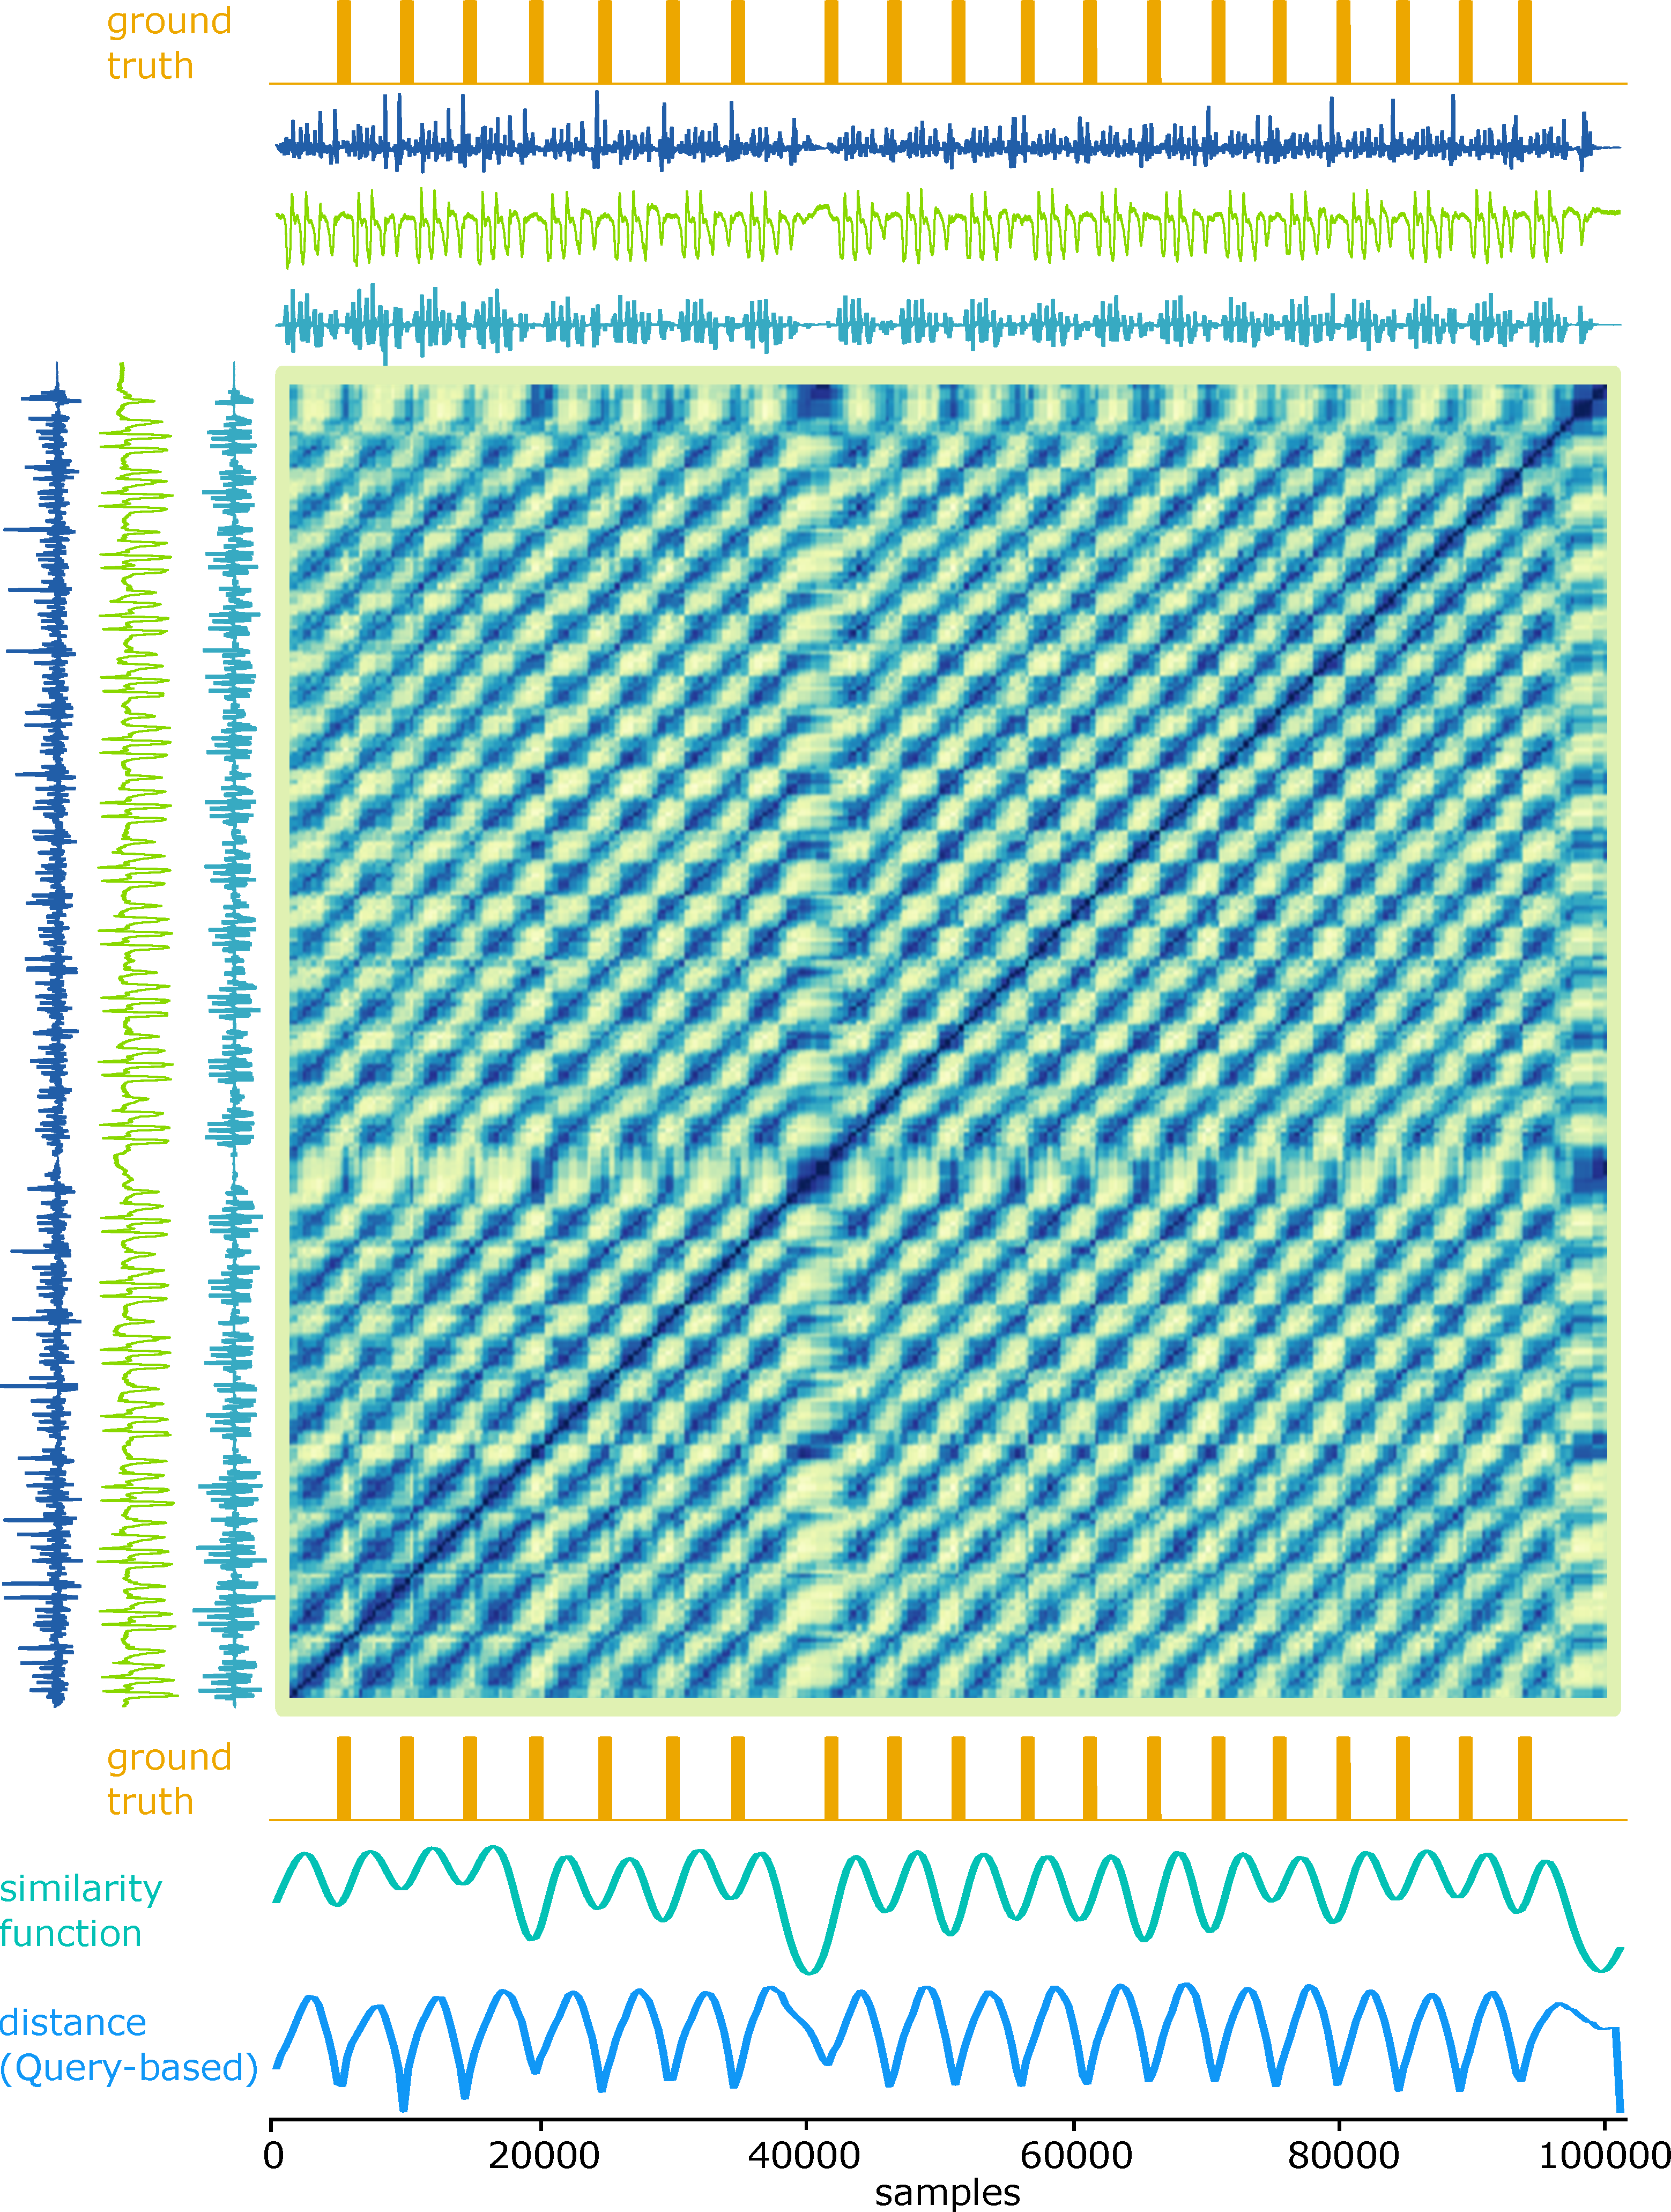
\includegraphics[width=\linewidth]{periodic_detection_example.pdf}
%\caption{Computing the \gls{ssm} of the periodic signal from subject 1, activity 0 (see Section \ref{dat:dataset12}). The ground truth is shown in orange (the first signal). The similarity function and distance profile from the query-based search are showed below the \gls{ssm}. The \gls{ssm} was computed with a window size of 5290 samples, and an overlap of 85\%.}
%\label{fig:periodic_detection}
%\end{wrapfigure}

\begin{figure}
\centering
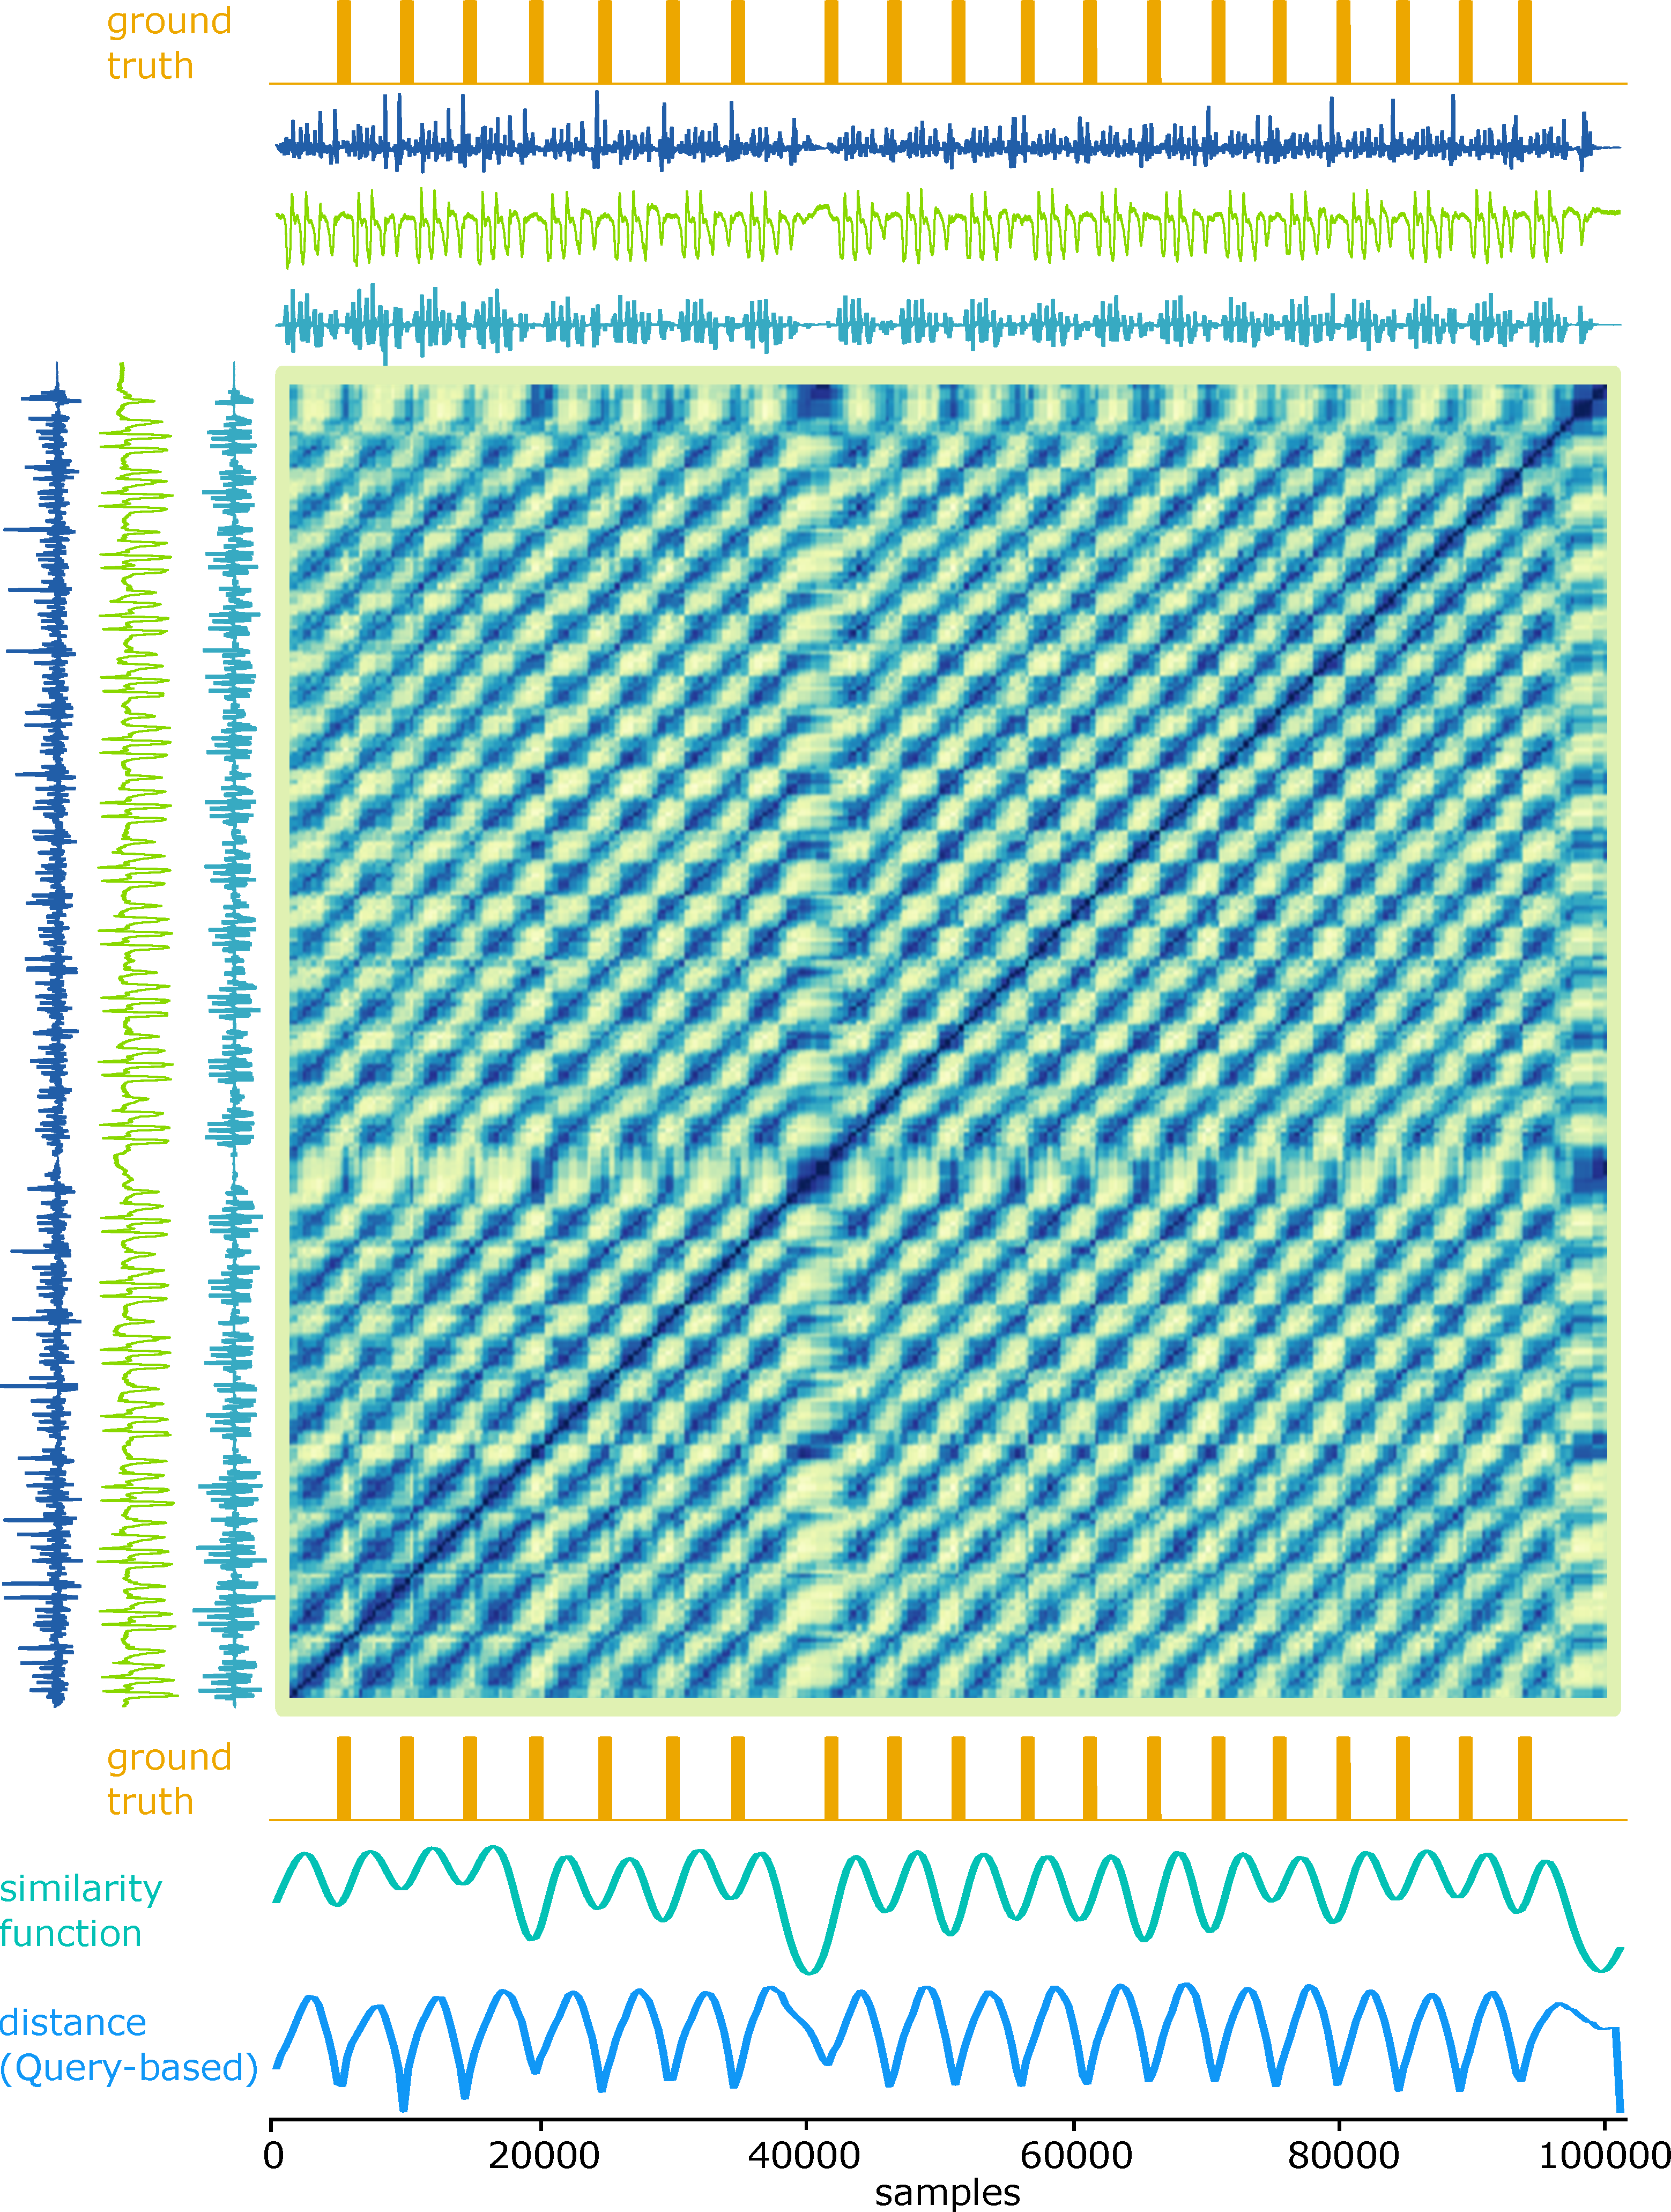
\includegraphics[width=0.75\linewidth]{periodic_detection_example.pdf}
\caption{Computing the \gls{ssm} of the periodic signal from subject 1, activity 0 (see Section \ref{dat:dataset12}). The ground truth is shown in orange (the first signal). The similarity function and distance profile from the query-based search are showed below the \gls{ssm}. The \gls{ssm} was computed with a window size of 5290 samples, and an overlap of 85\%.}
\label{fig:periodic_detection}
\end{figure}


The detection of periodic onset was experimented on Dataset 11 (\textit{CSL}, see Section \ref{dat:dataset12}). It is a database with exclusively periodic data of activity signals. Twenty participant performed seventeen different activities, which are recorded in a multimodal time series. We exemplify the usage of a periodic search with the similarity function and the query-based segmentation on the \gls{ssm}. These experiments were evaluated based on ground-truth annotations of a push-button from the dataset, with the metrics previously explained (see Section \ref{subsec:event_metrics}). The ground truth indicates the onset of the activity. Results are presented in Table \ref{tab:periodic_results}.

Using the similarity function enhances the periodic nature of the time series when computed (see Section \ref{sec:periodic_search}). The results are displayed for all activities, summing \textit{TP}, \textit{FP} and \textit{FN} of all participants. The periodic search was made using the window size of one period. The tolerance window was half the period length. The \textit{similarity function} was smoothed by a smoothing function (see Section \ref{subsec:smooth}) with a window size equal to the window size used to extract the features. The smoothing function helps in making the valley detection on the resulting similarity function easier and preventing unwanted \textit{FP}.

\begin{table}
\centering
\caption{Results in segmenting periodic data from dataset 11 (see Section \ref{dat:dataset12}). The results were computed with two different approaches on the \gls{ssm}: \textit{similarity function} and query-based search. \textit{TP}, \textit{FP}, \textit{FN }and resulting \textit{F1-score} were the metrics used. The total number of these metrics is presented on the last row.}
\begin{tabular}{lcccccccc}
\toprule
          & \multicolumn{4}{c}{Similarity function} & \multicolumn{4}{c}{Query-based search}\\
Activity &    TP &     FP &    FN &  F1-score &    TP &     FP &   FN &  F1-score \\
\midrule
0  &   348 &   37.0 &    33 &      0.91 &   375 &   15.0 &    6 &      0.97 \\
1  &   349 &   36.0 &    30 &      0.91 &   375 &   28.0 &    4 &      0.96 \\
2  &   323 &   39.0 &    58 &      0.87 &   381 &   48.0 &    0 &      0.94 \\
3  &   358 &   27.0 &    23 &      0.93 &   381 &   37.0 &    0 &      0.95 \\
4  &   335 &   17.0 &    39 &      0.92 &   372 &   35.0 &    2 &      0.95 \\
5  &   323 &   75.0 &    59 &      0.83 &   381 &   51.0 &    1 &      0.94 \\
6  &   365 &    4.0 &    16 &      0.97 &   380 &   13.0 &    1 &      0.98 \\
7  &   354 &   28.0 &    27 &      0.93 &   380 &   15.0 &    1 &      0.98 \\
8  &   336 &   25.0 &    44 &      0.91 &   364 &   35.0 &   16 &      0.93 \\
9  &   333 &   42.0 &    27 &      0.91 &   354 &   10.0 &    6 &      0.98 \\
10 &   341 &   31.0 &    40 &      0.91 &   379 &   17.0 &    2 &      0.98 \\
11 &   324 &   15.0 &    36 &      0.93 &   351 &   20.0 &    9 &      0.96 \\
12 &   682 &   74.0 &    52 &      0.92 &   718 &   68.0 &   16 &      0.94 \\
13 &   770 &   30.0 &   766 &      0.66 &   685 &  122.0 &  851 &      0.58 \\
14 &   322 &   50.0 &    40 &      0.88 &   353 &   41.0 &    9 &      0.93 \\
15 &   344 &   38.0 &    17 &      0.93 &   360 &   29.0 &    1 &      0.96 \\
16 &   584 &   60.0 &   126 &      0.86 &   659 &   26.0 &   51 &      0.94 \\
\midrule
Total &  6791 &  628.0 &  1433 &      0.89 &  7248 &  610.0 &  976 &      0.93\\
\bottomrule
\end{tabular}
\label{tab:periodic_results}
\end{table}


The results presented in Table \ref{tab:periodic_results} show that the similarity function can be used to segment periodic signals with a low rate of \textit{FP} and \textit{FN}. The overall F1-score is 0.89, being a good result but with margin for progress. The similarity function highlights this periodic behaviour, but the detection of periods is dependent on the ability to detect the relevant valleys. This process requires either a thresholding method (such as the one used on the novelty function) or the detection of all present valleys. Of course, using a valley/peak detection method with additional parameters, such as the distance between valleys/peaks, are plausible considering the nature of the problem. In this case, we used the simple approach of smoothing the signal and detecting all present valleys, with the risk of increasing \textit{FP} and/or \textit{FN} counts depending on the smoothing factor. Therefore, a better valley detection procedure can improve the current results. \textit{Activity 13} is an exception with a specially high rate of \textit{FN}, which is due to the nature of the ground-truth annotation. Figure \ref{fig:periodic_detection} illustrates an example of the periodic detection with the similarity function and the query-based search approach.

Although this method was mostly successful in segmenting the signal into distinctive periods. It does not always provide the moment where the \textit{path} starts on the \gls{ssm}. This moment should be the one detected to capture the true starting point of a period. The fact that we are not able to find the exact moment the \textit{path} starts means that an offset is present on the cycle detection. This is visible in Figure \ref{fig:periodic_detection}, where the valleys of the similarity function do not perfectly match the ground truth, when the \textit{paths} of the \gls{ssm} do. In the future, a different approach should be considered to segment the \textit{paths}. Nevertheless, the \gls{ssm} can still be used to segment periodic signals with the help of the analyst, by interactively selecting a segment of the signal as a query, or simply by indicating the index that corresponds to the beginning of the period, which is computed by query-based search with the \gls{ssm}' columns/rows, as explained in Section \ref{subsec:query_based_search}. This query-based search was also used in the same dataset and the results can be found in Table \ref{tab:periodic_results} and Figure \ref{fig:periodic_detection}. The query selected as template was the first period of the signal and the tolerance window equal to half the period size. The results show an expected improvement in the results, from 0.89 to 0.93 for the \textit{F1-score}. In this case, it is notorious that the \textit{FN} rate is much smaller than the previous case, which makes sense because a valley would always be present where the query overlaps each period.

It is also important to mention that this problem is not particularly complex for this dataset, considering that it is a controlled dataset with one periodic signal. But our intention with this experiment was to demonstrate the ability of the \gls{ssm} in (1) highlighting if a segment of the multimodal signal is periodic with the presence of \textit{paths}, and (2) segmenting the periods of this segment without any prior knowledge on the signal besides the window size, which is more flexible. Solely finding periodicity can be done with other methods, but in this case the \gls{ssm} shows all variations on a time series, with novelty and periodicity.

\subsection{Information Retrieval in Occupational Data}
\label{subsec:occupationa_examples}

The current information era, in conjunction with technological developments, is promoting a shift in the way industries and companies manage and perform their work. With the inclusion of sensing devices, dashboards and machine learning algorithms, many tasks can be better evaluated with direct quantitative measures. This can be made for machines to prevent breakdowns and optimize their performance, but can also be used for humans, specially to evaluate their occupational health, and prevent work-related disorders. This prevention implies a specialized intervention to perform changes in the workplace, the collaborator's training process and/or other organizational strategies. The process of deciding a need for intervention implies a previous risk evaluation of the collaborator's or team's routines. However, before the actual ergonomic risk evaluation, a considerable number of steps in preparing the data are needed. 

As we mentioned in Section \ref{sub:context2}, data preparation is an important part of any analysis or task that requires further deployment in supervised methods, namely the time-consuming segmentation and labelling processes. Hence, tools capable of segmenting time series to support and ease the labelling process of motion and posture data are highly valued and highly necessary for the risk analysis and the deployment of semi-supervised and/or supervised methods. In this case, motion data in real scenarios are even more complex since it is highly rich and diverse in behaviours. For instance, although cyclic and repetitive activities performed in industrial scenarios are mostly consistent from cycle to cycle, perfect conditions cannot be met all the time. Eventually, the working process can inadvertently be stopped or delayed. In addition, ergonomic risk assessment methods have to analyse each working cycle, which means that a previous segmentation of each one of these instances has to be made. Sub-activities that make the sequence of actions comprehended in the working cycle can also be sub-segmented for further recognition and association with risk measures. For instance, the \textit{ergonomist} might have an interest in understanding which actions from the working cycle have a significant association with a high or low risk measure, and adapt the working station with intervention strategies that could help prevent future disorders. 

In this Section, we explore a few examples in using the \gls{ssm} for information retrieval in occupational motion data of collaborators performing specific workstations. The data was recorded at the \textit{Autoeuropa Volkswagen} production line (Dataset 13, \textit{VAOD}, see Section \ref{dat:dataset_industry}). The information provided by the \gls{ssm} supports the analyst in identifying the following events: 

\begin{itemize}
\label{items:occupational_detection}
    \item \textbf{Active working periods:} \textit{Active and non-active segments} indicate sub-sequences of the time series where the collaborator was performing the cyclic working tasks or not (e.g.: stop on the working line that leads to a pause in the working activity). With this information, we can focus the attention to active working periods, which are the segments of interest to perform risk analysis. For this, the \textit{novelty function} can provide the moments of change between active and non-active regimes, as we will show further;
    
    \item \textbf{Working cycles:} Sub-sequences of highly similar sequences of movements that are being repeated in time. This type of segmentation pre-assumes that the time series under analysis will be mostly (or entirely) defined by the repetition of a motion. The illustrated examples show only tasks that are cyclic. The \textit{similarity function} highlights moments with periodic behaviour.
    
    \item \textbf{Sub-cyclic segments:} Sub-cyclic segments inside each working cycle can be compared to evaluate how much it contributes to the risk score of a workstation. Segmenting the same portion of the working cycle over time can provide relevant comparative measures for decision making or intervention in the production line (e.g. it can be decided that the portion of the cycle has to be change to reduce the exposure to risk factors). The usage of a query-based mechanism with an example of the \textit{subsequence} is used to demonstrate the findings.
\end{itemize}


\subsubsection{Novelty and Periodic Segmentation in Occupational Data}

\begin{figure}
 \begin{subfigure}{0.45\linewidth}
      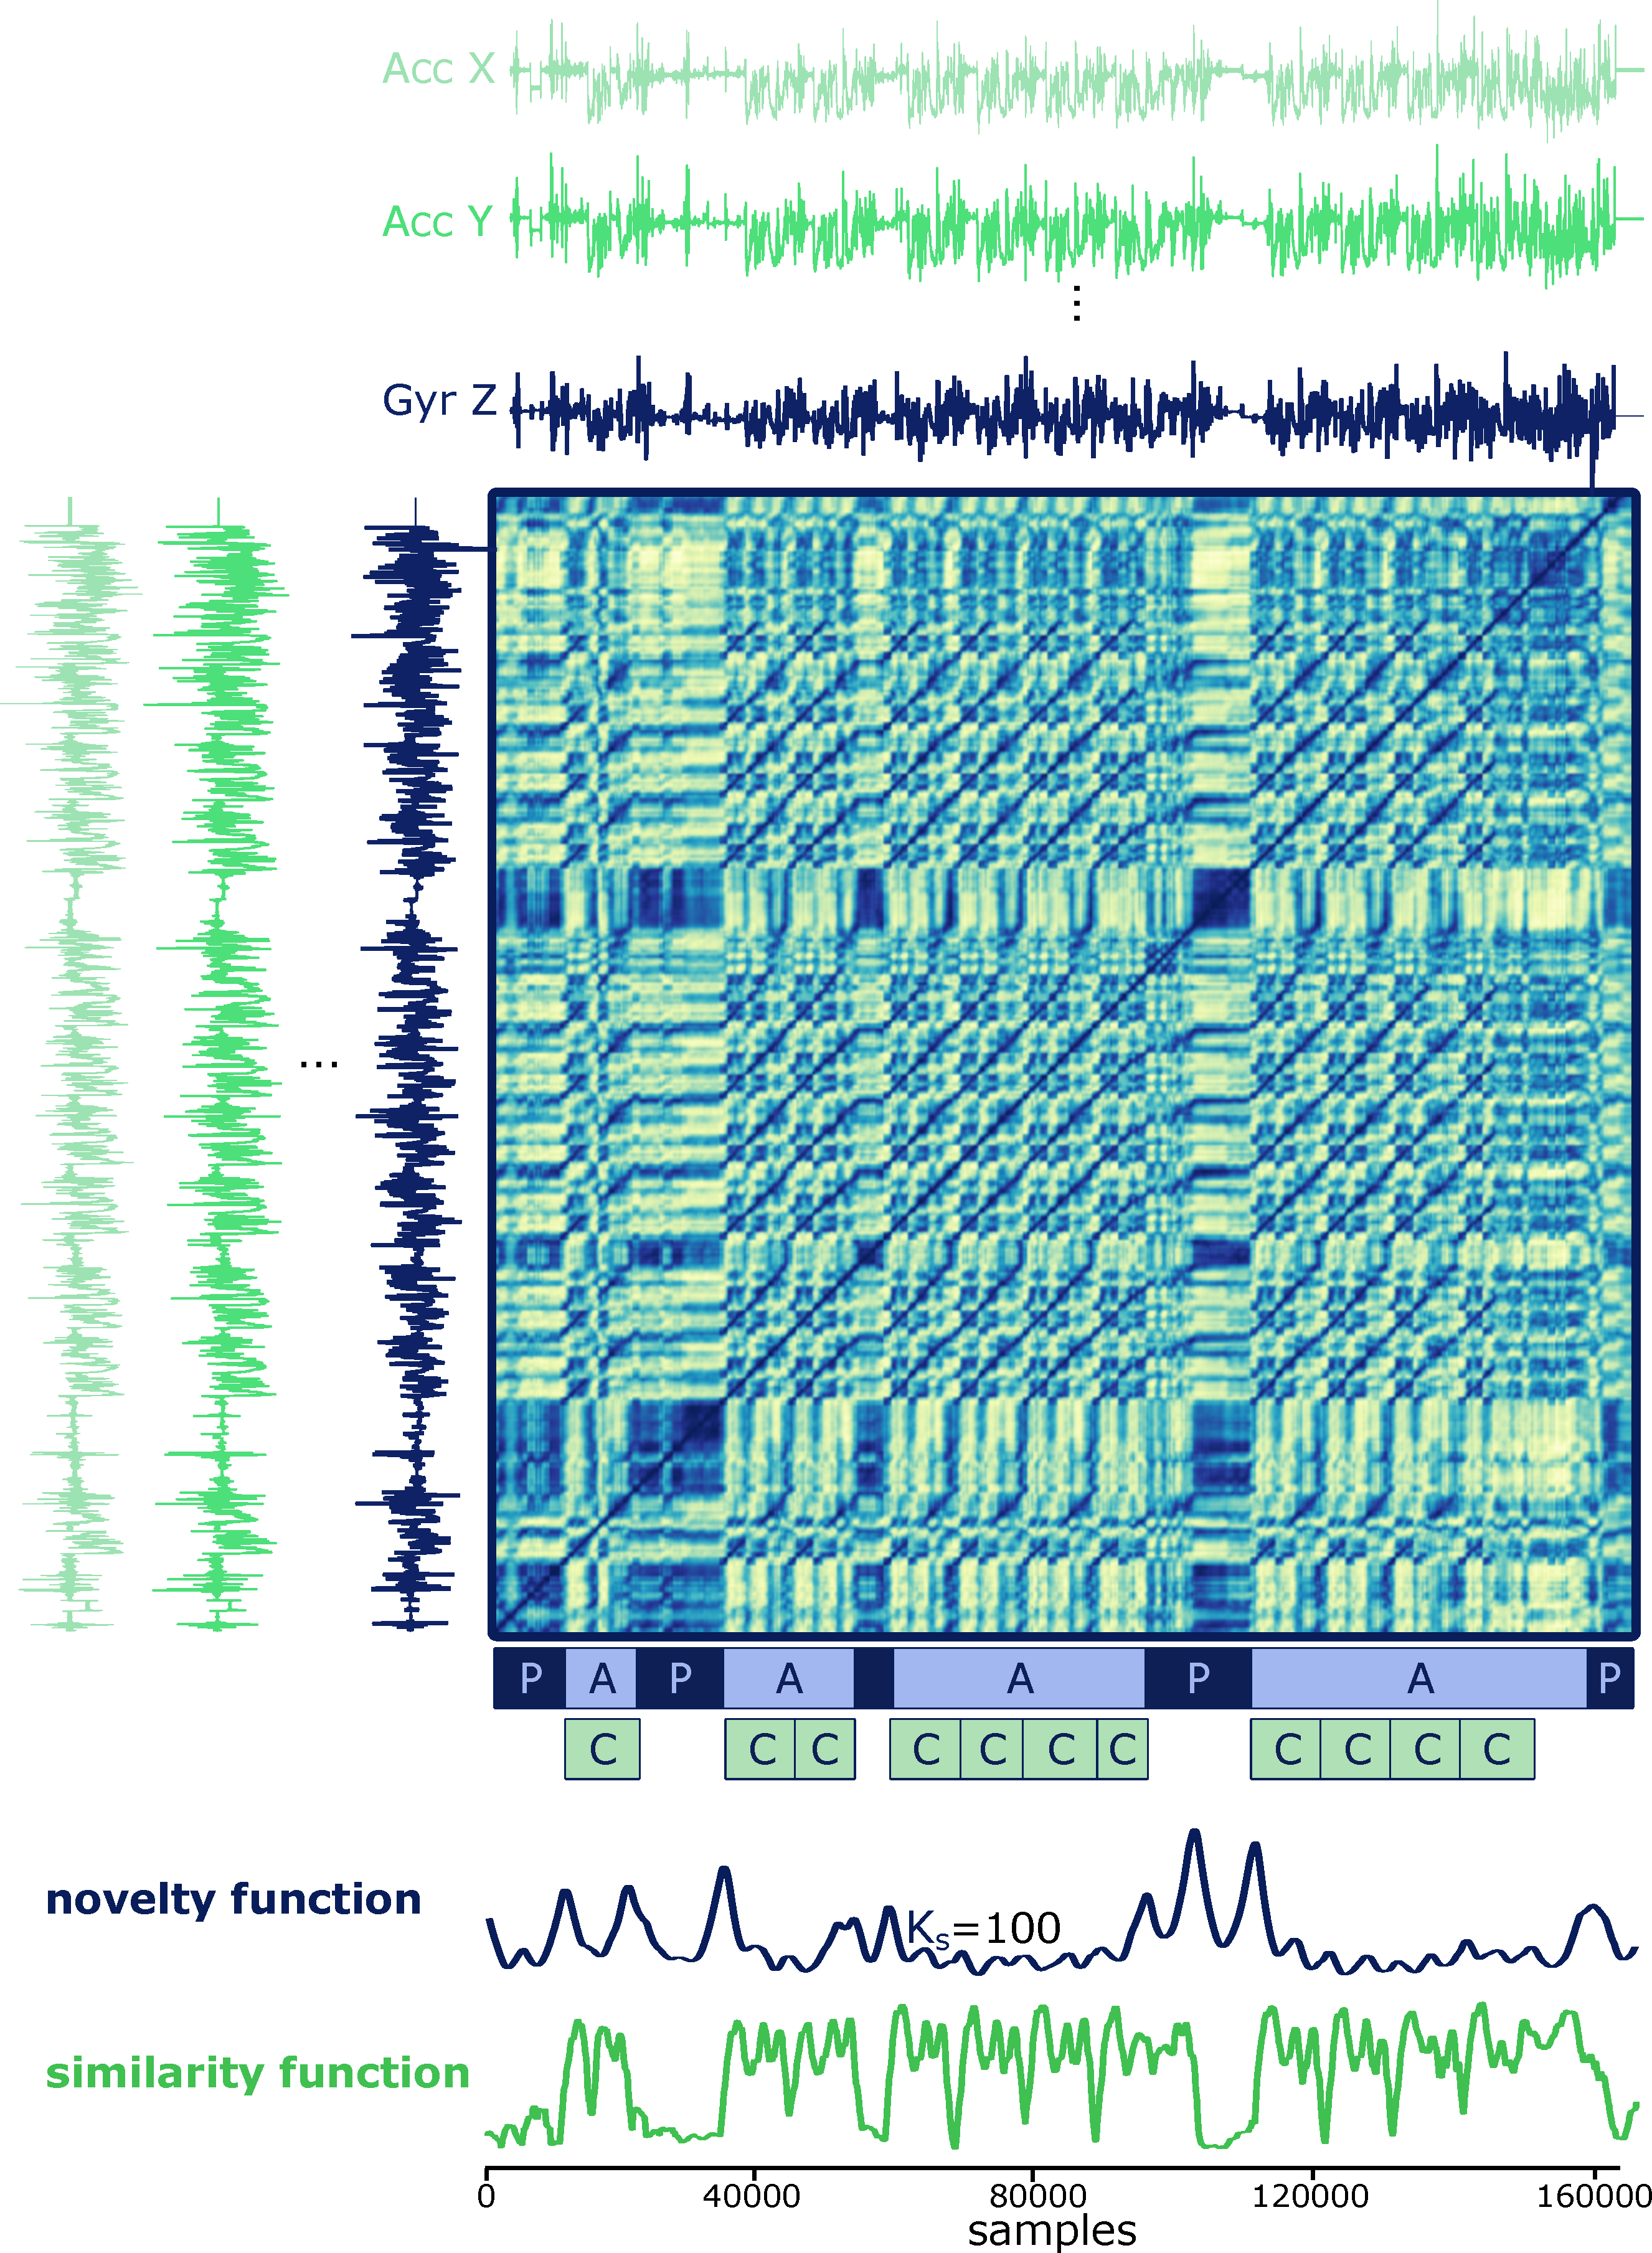
\includegraphics[width=\textwidth]{AE_example1.pdf}
  \caption{}
  \label{fig:ae_example1}
 \end{subfigure}
 \begin{subfigure}{0.45\linewidth}
      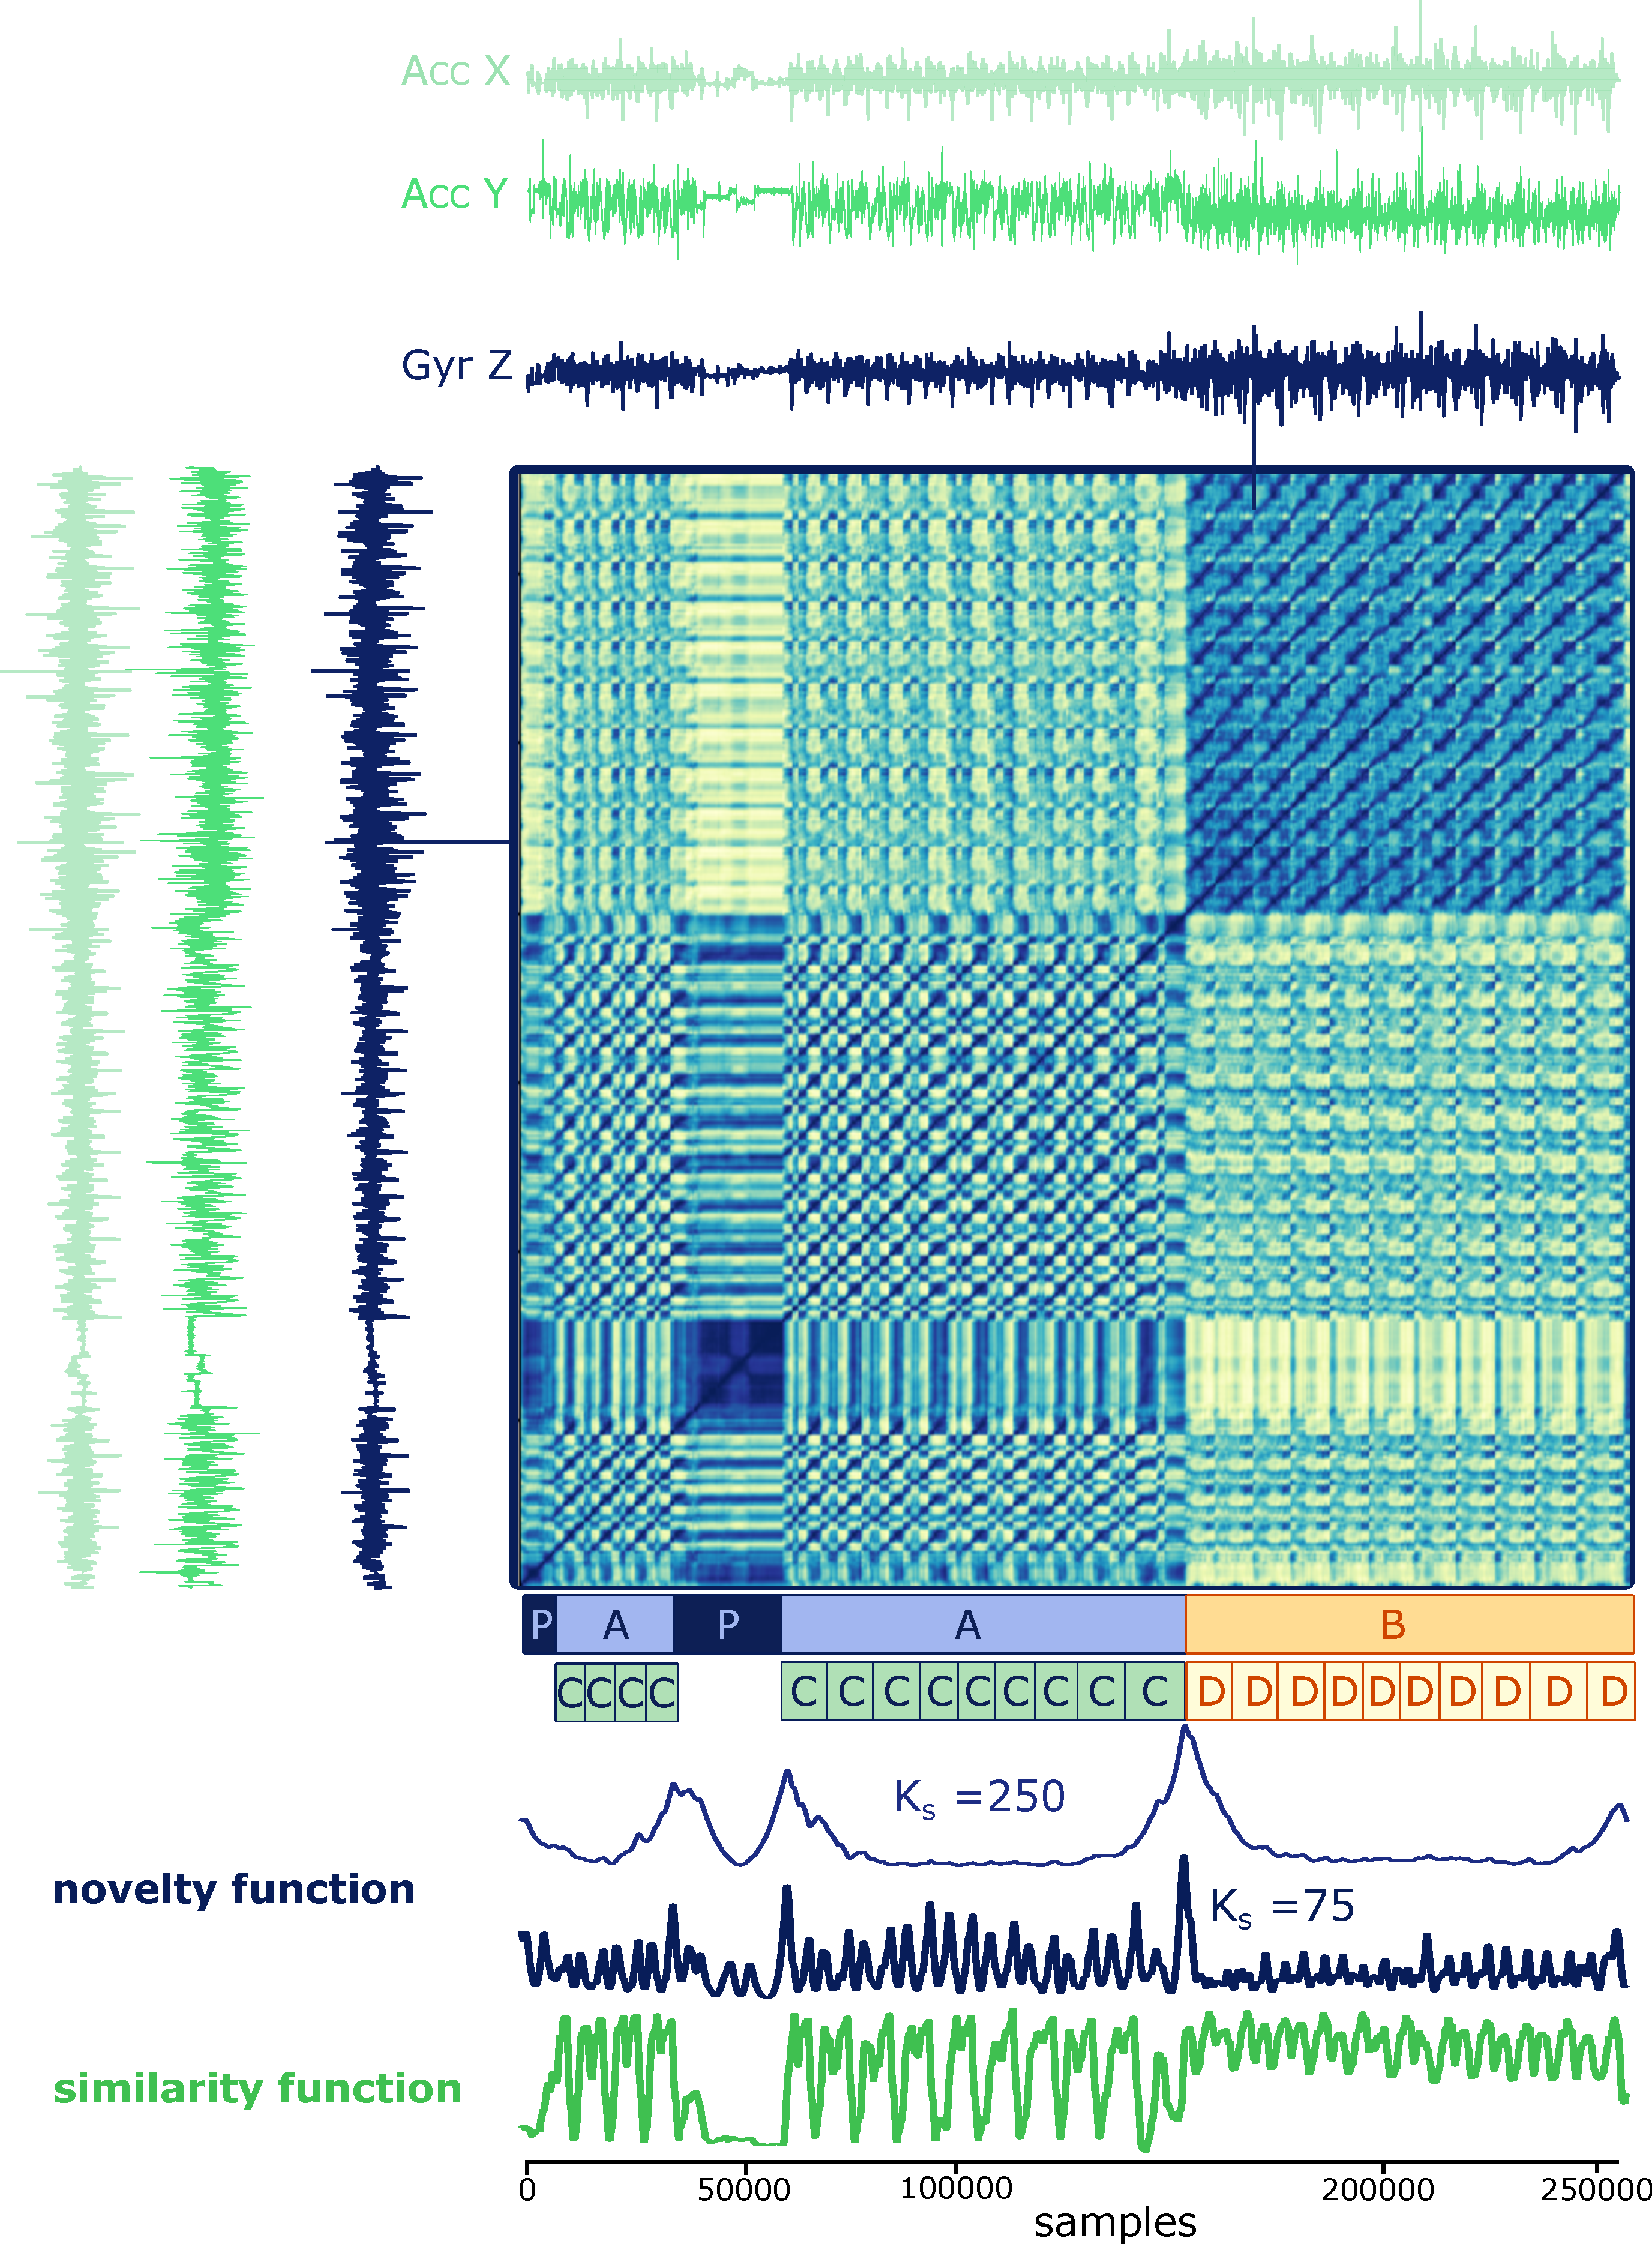
\includegraphics[width=\textwidth]{AE_example2.pdf}
  \caption{}
  \label{fig:ae_example2}
  \end{subfigure}
\caption{Illustrative examples that show how to use the \gls{ssm} for information retrieval in motion data of occupational scenarios. In both figures, a set of signals, presented as \textit{Acc X, Y} and \textit{Gyr Z} show a sample of the data used (Acc is the \gls{acc} and Gyr is the \gls{gyro} data). The data from the wrist and elbow were used for this analysis. The segments are illustrated and labelled below the \gls{ssm} with \textit{\textbf{P} - interruption/pause in the production line}, \textit{\textbf{A} - active working period}, \textit{\textbf{C} - working cycle}, \textit{\textbf{B} - active working period for workstation 2} and \textit{\textbf{D} - working cycle 2}. The novelty and similarity functions are presented to show the match with the segmentation labels. In (a), the signal represent a collaborator performing one workstation with interruptions, while in (b) a collaborator working in two different workstations.}
\end{figure}

In Figures \ref{fig:ae_example1} and \ref{fig:ae_example2} we present two different examples of data acquired while the collaborators were working. In Figure \ref{fig:ae_example1}, collaborator 1 was performing the cyclic task 1, while in Figure \ref{fig:ae_example2}, collaborator 2 was performing two different tasks (1 and 2). It is clear in both Figures that the \gls{ssm} provides a visual feedback that highlights moments where the signal change (\textit{blocks}), as well as where cycles occur (\textit{paths}). In the first case, the collaborator waited (\textbf{P}) to start the task (\textbf{A}), up until the collaborator was interrupted several times by a stoppage on the production line to then continue his/her tasks. The novelty function is able to detect all of these main transitions, while the similarity function highlights where the working cycles (\textbf{C}) are.

In the second example, collaborator 2 was performing the same workstation  (\textbf{A}) as collaborator 1 but shifted to another workstation (\textbf{B}). The \gls{ssm} indicates well when transitions occur, namely where the collaborator was interrupted while performing workstation \textbf{A}, and when shifting to workstation \textbf{B}. This is highlighted with the novelty function. The cycles are also visible with \textit{paths}, for both workstations. The similarity function highlights well where the working cycles (\textbf{C} and \textbf{D}) happen. However, the search for working cycles should be performed after a first segmentation between homogeneous segments in order to have better results. 

It is also relevant to mention that when the collaborator is in non-active periods (\textbf{P}), the \textit{similarity function} has a very low value. As we mentioned in Section \ref{sec:periodic_search}, a low similarity function value also corresponds to being very dissimilar to all the other \textit{subsequences} of the signal. In this case, it makes sense, considering that the majority of the signal is related with cyclic activities, being \textbf{P} instances less frequent and therefore less similar with all the other \textit{subsequences}. This happens in both examples.

The \textit{novelty} and \textit{similarity} functions were used with the purpose of detecting the listed events (see List \ref{items:occupational_detection}) on Dataset 13 (\textit{VAOD}, see Section \ref{dat:dataset_industry}). For the sake of brevity, the results for both item one and two of the list are displayed in Appendix \ref{appendix:tables_detailed} (see Tables \ref{tab:auto_scores} and \ref{tab:wc_results}, respectively). The first step involved detecting changes between active and non-active periods of the working activity, which was performed with the novelty function. The periods were described as active or non-active based on a threshold on the similarity function. The results show the ability to segment the signals with an overall F1-score of 0.96 (see Table \ref{tab:auto_scores}). After identifying the active periods, working cycles were segmented. From the 157 working cycles, 154 cycles were detected (see Table \ref{tab:wc_results}). 

\subsubsection{Query-based Segmentation in Occupational Data}

\begin{figure}
  \centering
      \includegraphics[width=\textwidth]{AE_example3.pdf}
  \caption{Illustrative example that shows how to use the \gls{ssm} for information retrieval in motion data of occupational scenarios. The query-based search with a template is made on the \gls{ssm} of the signal. This search procedure highlights where the query re-occurs on the signal with the distance functions (\textit{subsegment 1} and \textit{subsegment 2}). The templates are highlighted on the signal (Acc X) and on the right of the resulting subsegments. The small thumbnails next to the template illustrates the actions being performed on the cycle by the collaborator (highlighted in blue) and the tool being used (highlighted in orange). On the first subsegment, the collaborator was reaching over the head and pulling down the working tool, while on the second subsegment, the collaborator was screwing the pieces on the side of the car.}
  \label{fig:ae_example3}
\end{figure}

Another aspect of occupational risk evaluation in industrial scenarios is to compare the exposure to risk factors of sub-segments of the working cycle. This strategy could support professionals in identifying specific sequences of sub-activities that occur in-cycle, and search them over the entire set of working cycles for comparative purposes. In Figure \ref{fig:ae_example3} we show an example where the subsequence search matches exactly two distinctive in-cycle patterns (1 - blue; and 2 - green) of the working activity. Using these subsequences as a query template, we can match their onset over the successive cycles by finding the major valleys of the resulting distance functions (see Equation \ref{eq:subsec_search}).

\section{Pattern Search with SSTS}

In order to show the value of using a symbolic representation of the time series and search with \gls{regex} on that representation, we provide six examples of how to use \gls{ssts} for pattern search on time series and compare the text complexity between the python implementation and the query used, with Halstead measures. 

\subsection{Illustrative Evaluation of SSTS in Various Application Scenarios}

We will present six examples (three more detailed): the second and third examples consist of simple problems that require the detection of local maxima and minima. The sixth example is a more challenging task, which requires the usage of more sophisticated mechanisms of the \gls{regex} module. The examples are listed as follows(\textit{Example 1} is omitted since it was discussed in the previous section):

\begin{itemize}
\item Example 2 - Step Detection: Detect the instants in time when a right or left heel floor contact is achieved during a normal straight walk from the magnitude of an accelerometer signal. This information can be used to create a step detector based on accelerometer data. Since the sensor is located on the right pocket, global minima will indicate the right heel contact and local minima will correspond to left heel contact;

\item Example 3 - Segmentation of the systole of the \gls{abp} wave: The dicrotic notch corresponds to the physiological event of the aortic valve closure, which triggers the increase of the aortic pressure and signifies the end of the systolic phase. In this problem, it is asked to segment the systolic phase of the \gls{abp} wave;

\item Example 4 - Electrocardiogram peak detector: Detect all the major peaks from an \gls{ecg} record;

\item Example 5 - Straight Line Trajectory Tracking: The automatic detection of trajectory features, such as straight walks and turns can be used to evaluate trajectory anomalies from a vector of cartesian coordinates in 2D-space;

\item Example 6 - Since the first 5 s of the lifting exercise are unstable, the problem involves detecting the first stable lifting step, which occurs approximately 5 s after the beginning of the exercise from an accelerometer signal.

\end{itemize}

For the sake of brevity, only three of the examples are presented.

\subsubsection{Example 2 - Step Detection in accelerometer signals}

In this particular case, only the detection of the right heel contact will be discussed, whereas the left heel contact example's solution is presented in Table \ref{tab:Summary}.

\begin{figure}[H]
  \centering
      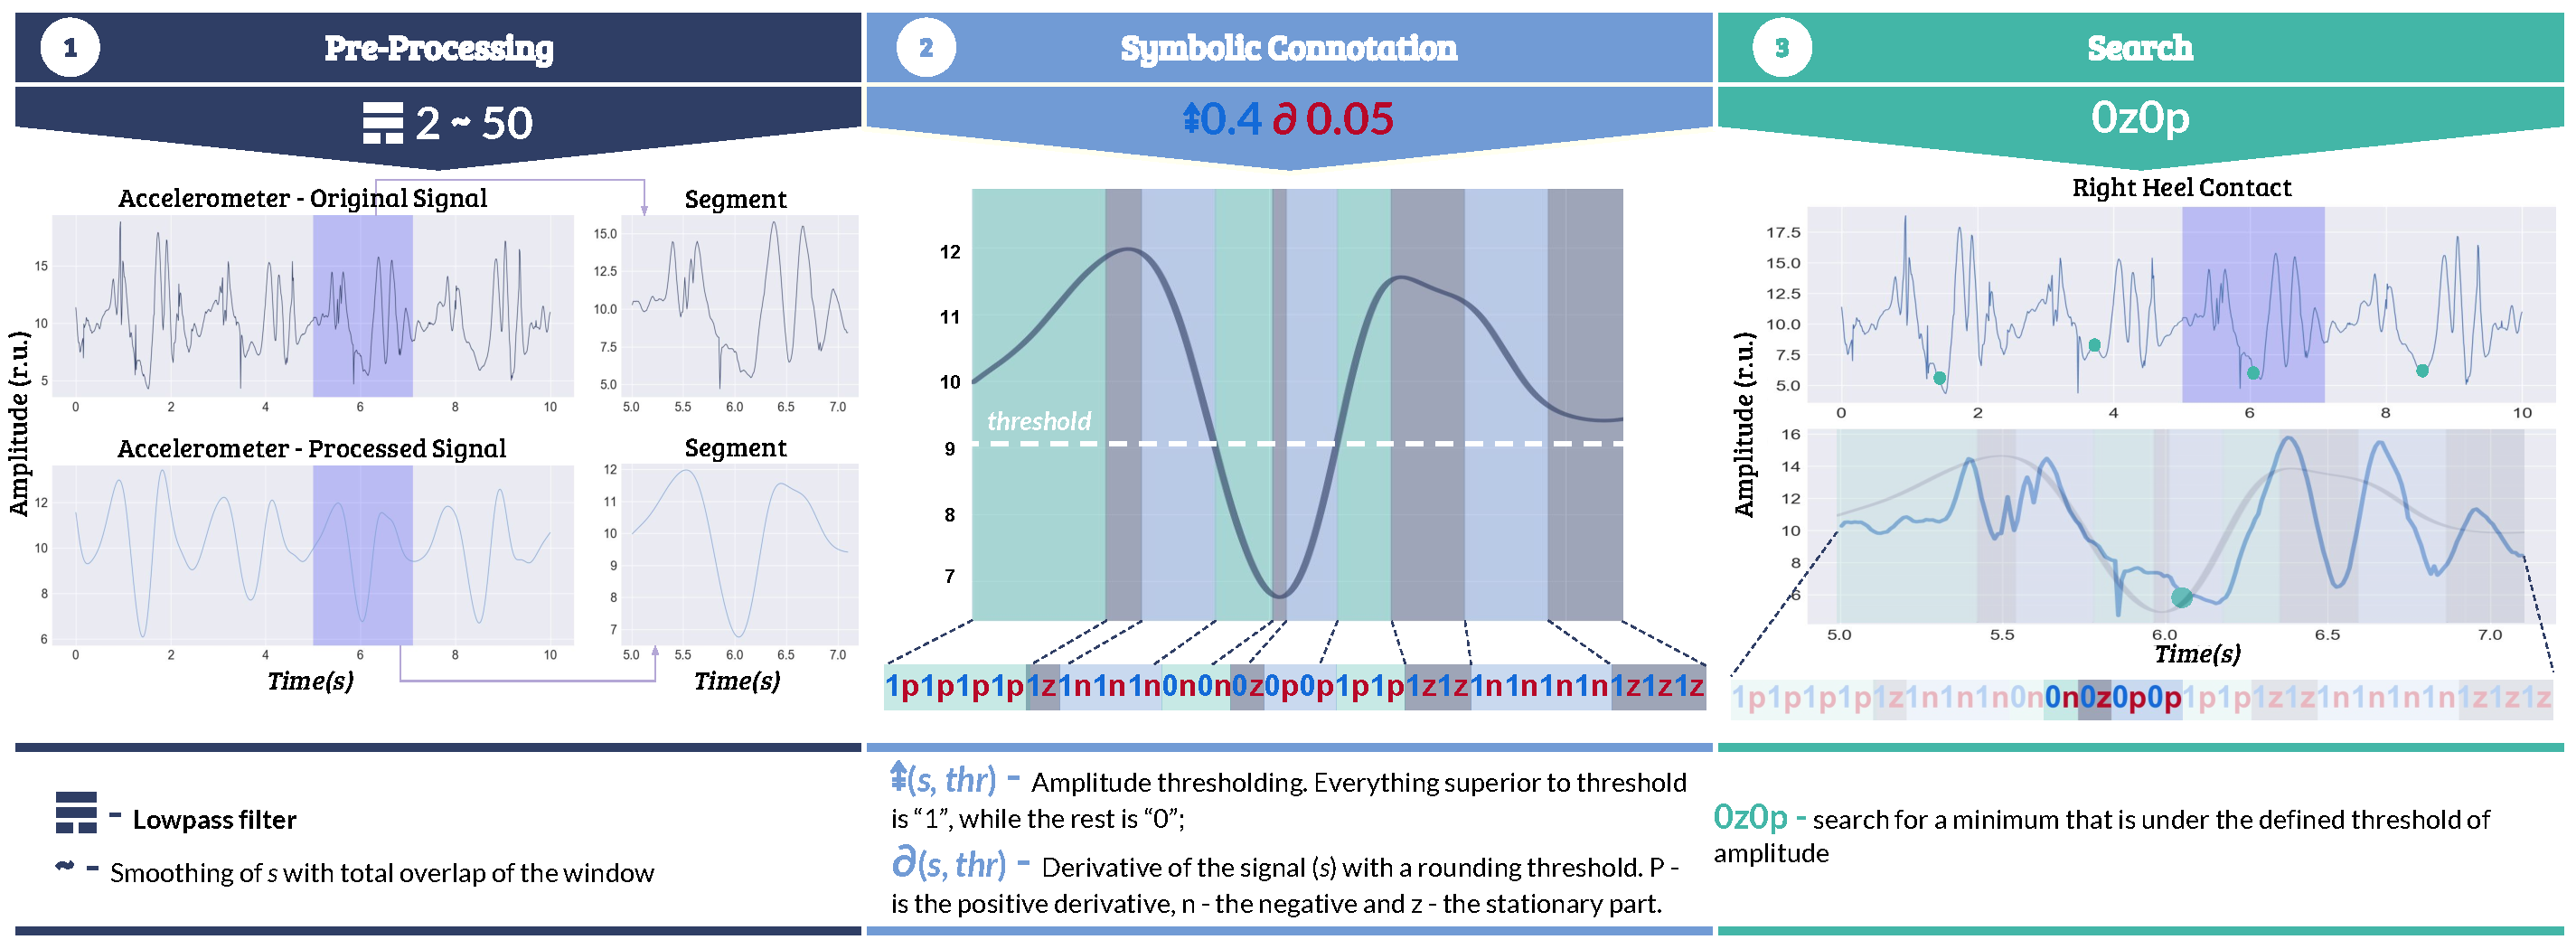
\includegraphics[width=\textwidth]{ssts_example2.pdf}
  \caption{Example 2 - Solution pipeline of Step Detection example. At the bottom of the figure are summarized the operators and methods used in each step. In the symbolic connotation step, the alternation between the methods is made with colors (Blue - A - Amplitude Comparison, Red - D1 - First Derivative). A dotted line is shown to represent the threshold level. Each color band in the signal corresponds to a specific primitive. A positive match is highlighted with green in the search step.}
  \label{fig:Exercise2}
\end{figure}

The signal is initially pre-processed to ease the identification of the subject's steps. This is achieved using a low pass filter (\textbf{LP}). The result is presented in the second image of the first step in Fig. \ref{fig:Exercise2}. A highlight is also present and delineates a segment of the signal that has a minimum peak, which corresponds to right heel contact. The string representation of this segment is depicted in the second step.
\par
The string is a sequence of primitives composed of two connotation methods (\textbf{A} in blue, \textbf{D1} in red). Based on these methods, the samples of the signal with amplitudes greater than \textit{40}\% of the range amplitude are transcribed into $1$, while the remaining turn into $0$; the slopes are converted into $p$, $z$ and $n$, when rising, being stationary and falling, respectively.
\par
The solution involves detecting each minimum with an amplitude inferior to the threshold level. The morphological representation of a minimum can be reduced to a negative slope followed by a positive one, which in the symbolic representation is defined by the second connotation method as the transition from \texttt{n} to \texttt{p} or \texttt{z} to \texttt{p}. Regarding the amplitude requirement, it is assigned by the first connotation method, in which any value lower than the threshold level is \texttt{0}. The \gls{regex} used to find this minimum was \texttt{0z0p}, which implies that: (1) the amplitude has to be \texttt{0}; and (2) the derivative is \texttt{z} and then \texttt{p}. The detection is highlighted in green in the last plot of Fig. \ref{fig:Exercise2}.

\subsubsection{Example 3 - Dicrotic notch detection in ABP signals}

The \gls{abp} waves are morphologically represented by a high positive slope that corresponds to the systolic uptake and ends at the peak of the systolic pressure. After this behaviour, follows the systolic decline, which ends with the aortic valve closure, named the \textit{dicrotic notch} in the signal representation~\cite{abpSignal}.
\par
These types of signals are commonly affected by low-frequency noise that modulates the signal and is contaminated with high-frequency noise of low amplitude. The typical procedure is to bandpass the \gls{abp} signal to remove both types of noise. Fig. \ref{fig:Exercise3} depicts how a band pass filter that cuts frequencies under 1 Hz and above 20 Hz (BP) is applied to the signal to remove both types of noise. The modulation removal is shown with the linear regression in both original and pre-processed signals, which in the first case has a positive slope and after the pre-processing is approximately zero.

\begin{figure}
  \centering
      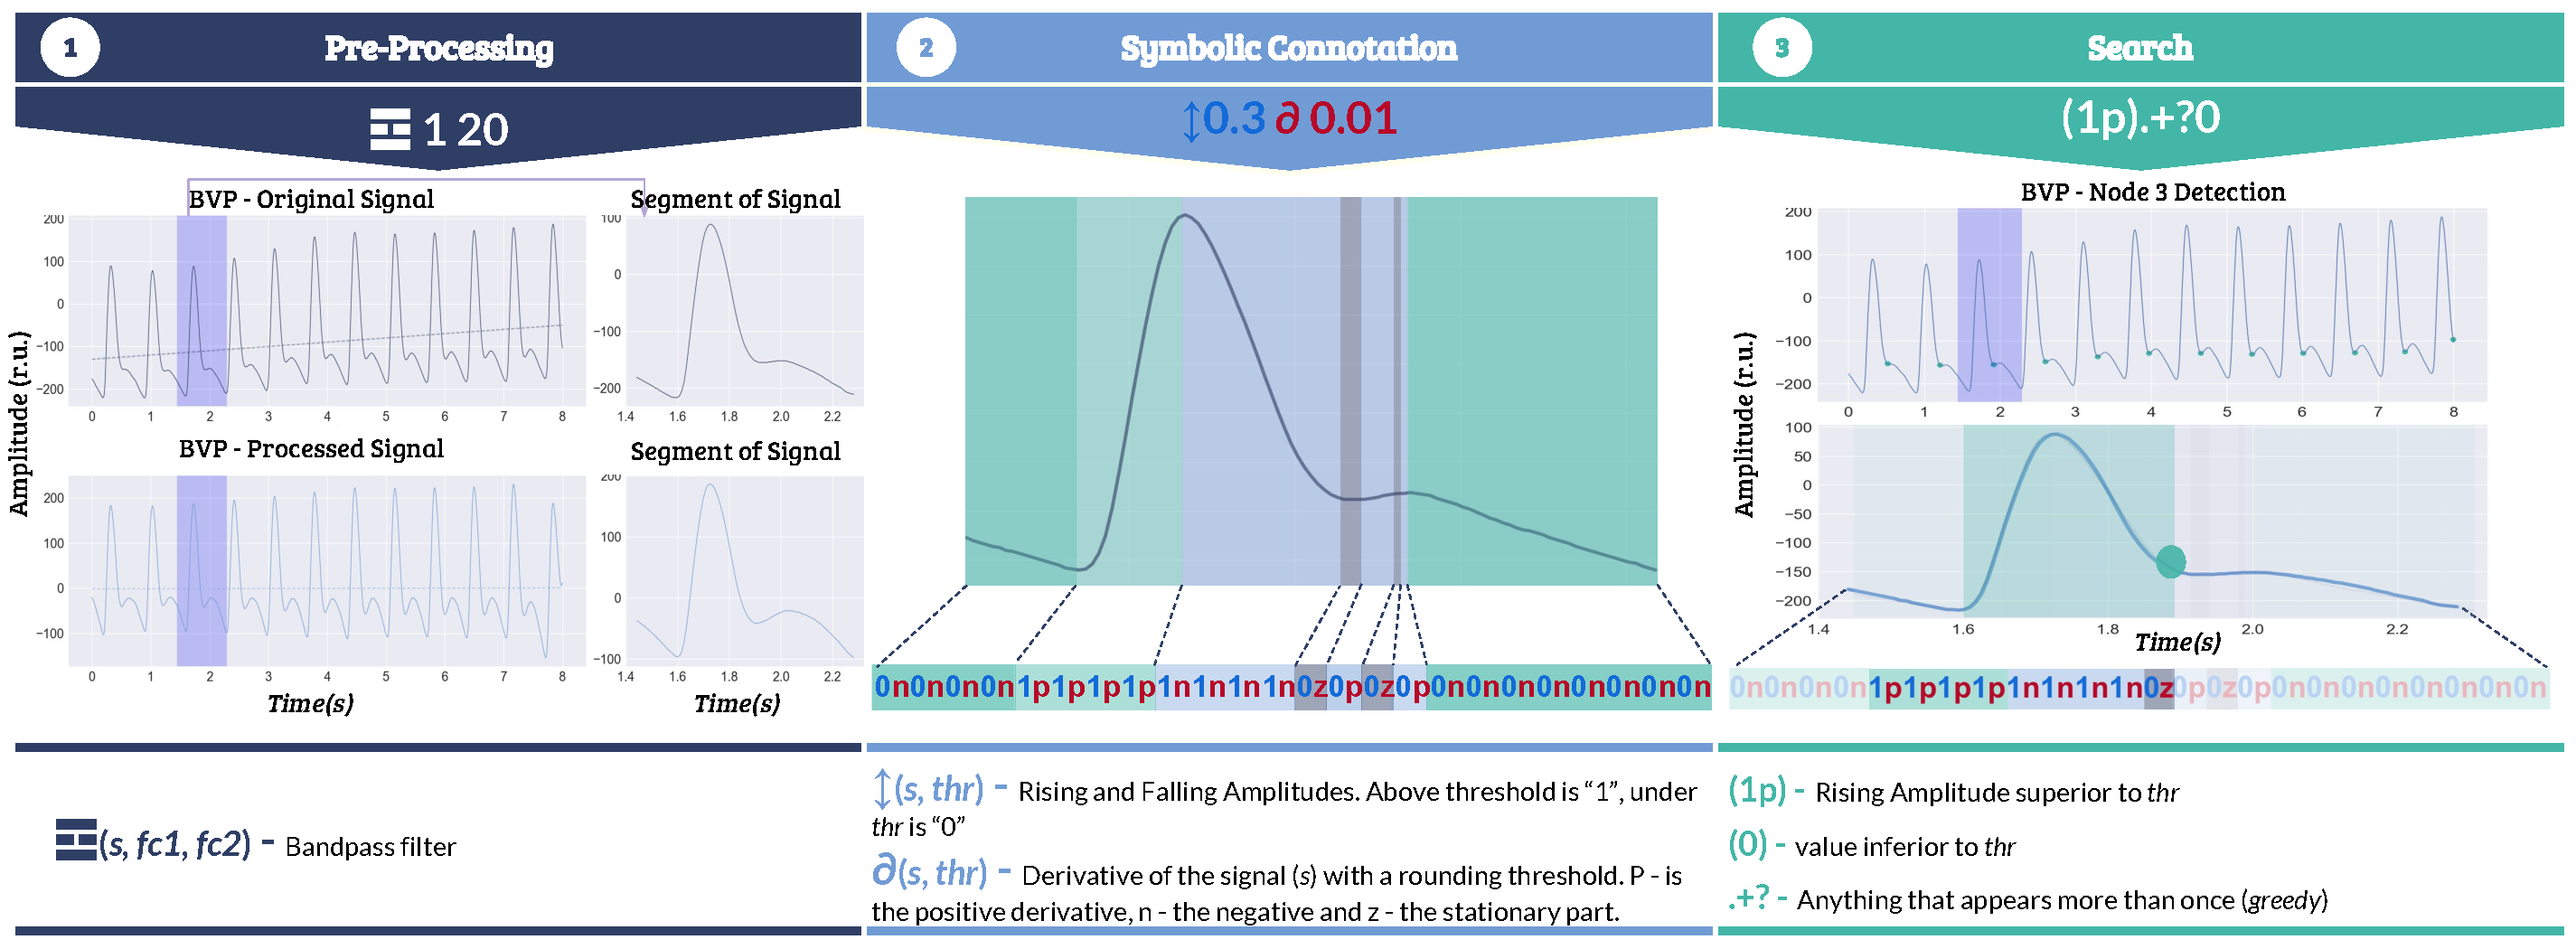
\includegraphics[width=\textwidth]{ssts_example3.pdf}
  \caption{Example 3 - Solution pipeline of Dicrotic notch detection example. The operators or methods used in each step are summarized at the bottom of the figure. In the symbolic connotation step, the alternation between methods is represented with colors (Blue - AD, Red - D1). For each color band in the signal, there is a corresponding primitive. The match is highlighted with green in the search step.}
  \label{fig:Exercise3}
\end{figure}

In the symbolic connotation step, the reasoning follows the signal morphological description and uses two methods for the symbolic representation. The first, AD (represented in blue), detects all rising and falling slopes that are higher than a specific threshold (in this case 30\% of the amplitude range of the signal) and transcribes the sample values to \texttt{1}, while the remaining values are converted to $0$. The second method (represented in red) uses the derivative, as mentioned in the previous examples.
\par
The first connotation method is necessary to distinguish between the rising slope that occurs at the beginning of the pressure wave and the one after the \textit{dicrotic notch}. With this distinction, it is possible to find the beginning of the \gls{abp} wave as a high positive slope (\texttt{1p}) and find the \textit{dicrotic notch} when the lower slope starts (\texttt{0.}). In order to find this area of the \gls{abp} wave, the \gls{regex} has to start with the first \texttt{1p} primitive and end with the first \texttt{0.} primitive. 

\par
The example is solved with the following \gls{regex}: \texttt{(1p).*?(0.)}. This string means that the search will match anything (represented by "\texttt{.*?}") between the first "\texttt{1p}" primitive and the first "\texttt{0.}" primitive.

\subsubsection{Example 6 - Stable lifting detection in accelerometer signals}

In the previous example, the solution was achieved by searching for one simple transition in the string generated by the sequence of connotation methods. This tool may also be used to solve more complex examples in the same manner.
\par
The next problem involves the segmentation of a lifting step that has occurred 5 seconds after the start of a weight lifting exercise. The example can be solved in two steps: (1) find the start of the exercise, and (2) search for the segment 5s after the start. This rationale can be expressed by combining two distinct symbolic representations of the same original signal, which requires the use of two pre-processing and symbolic connotation sets, in which one is used for the detection of the start and the other to find the desired segment.

\begin{figure}
  \centering
      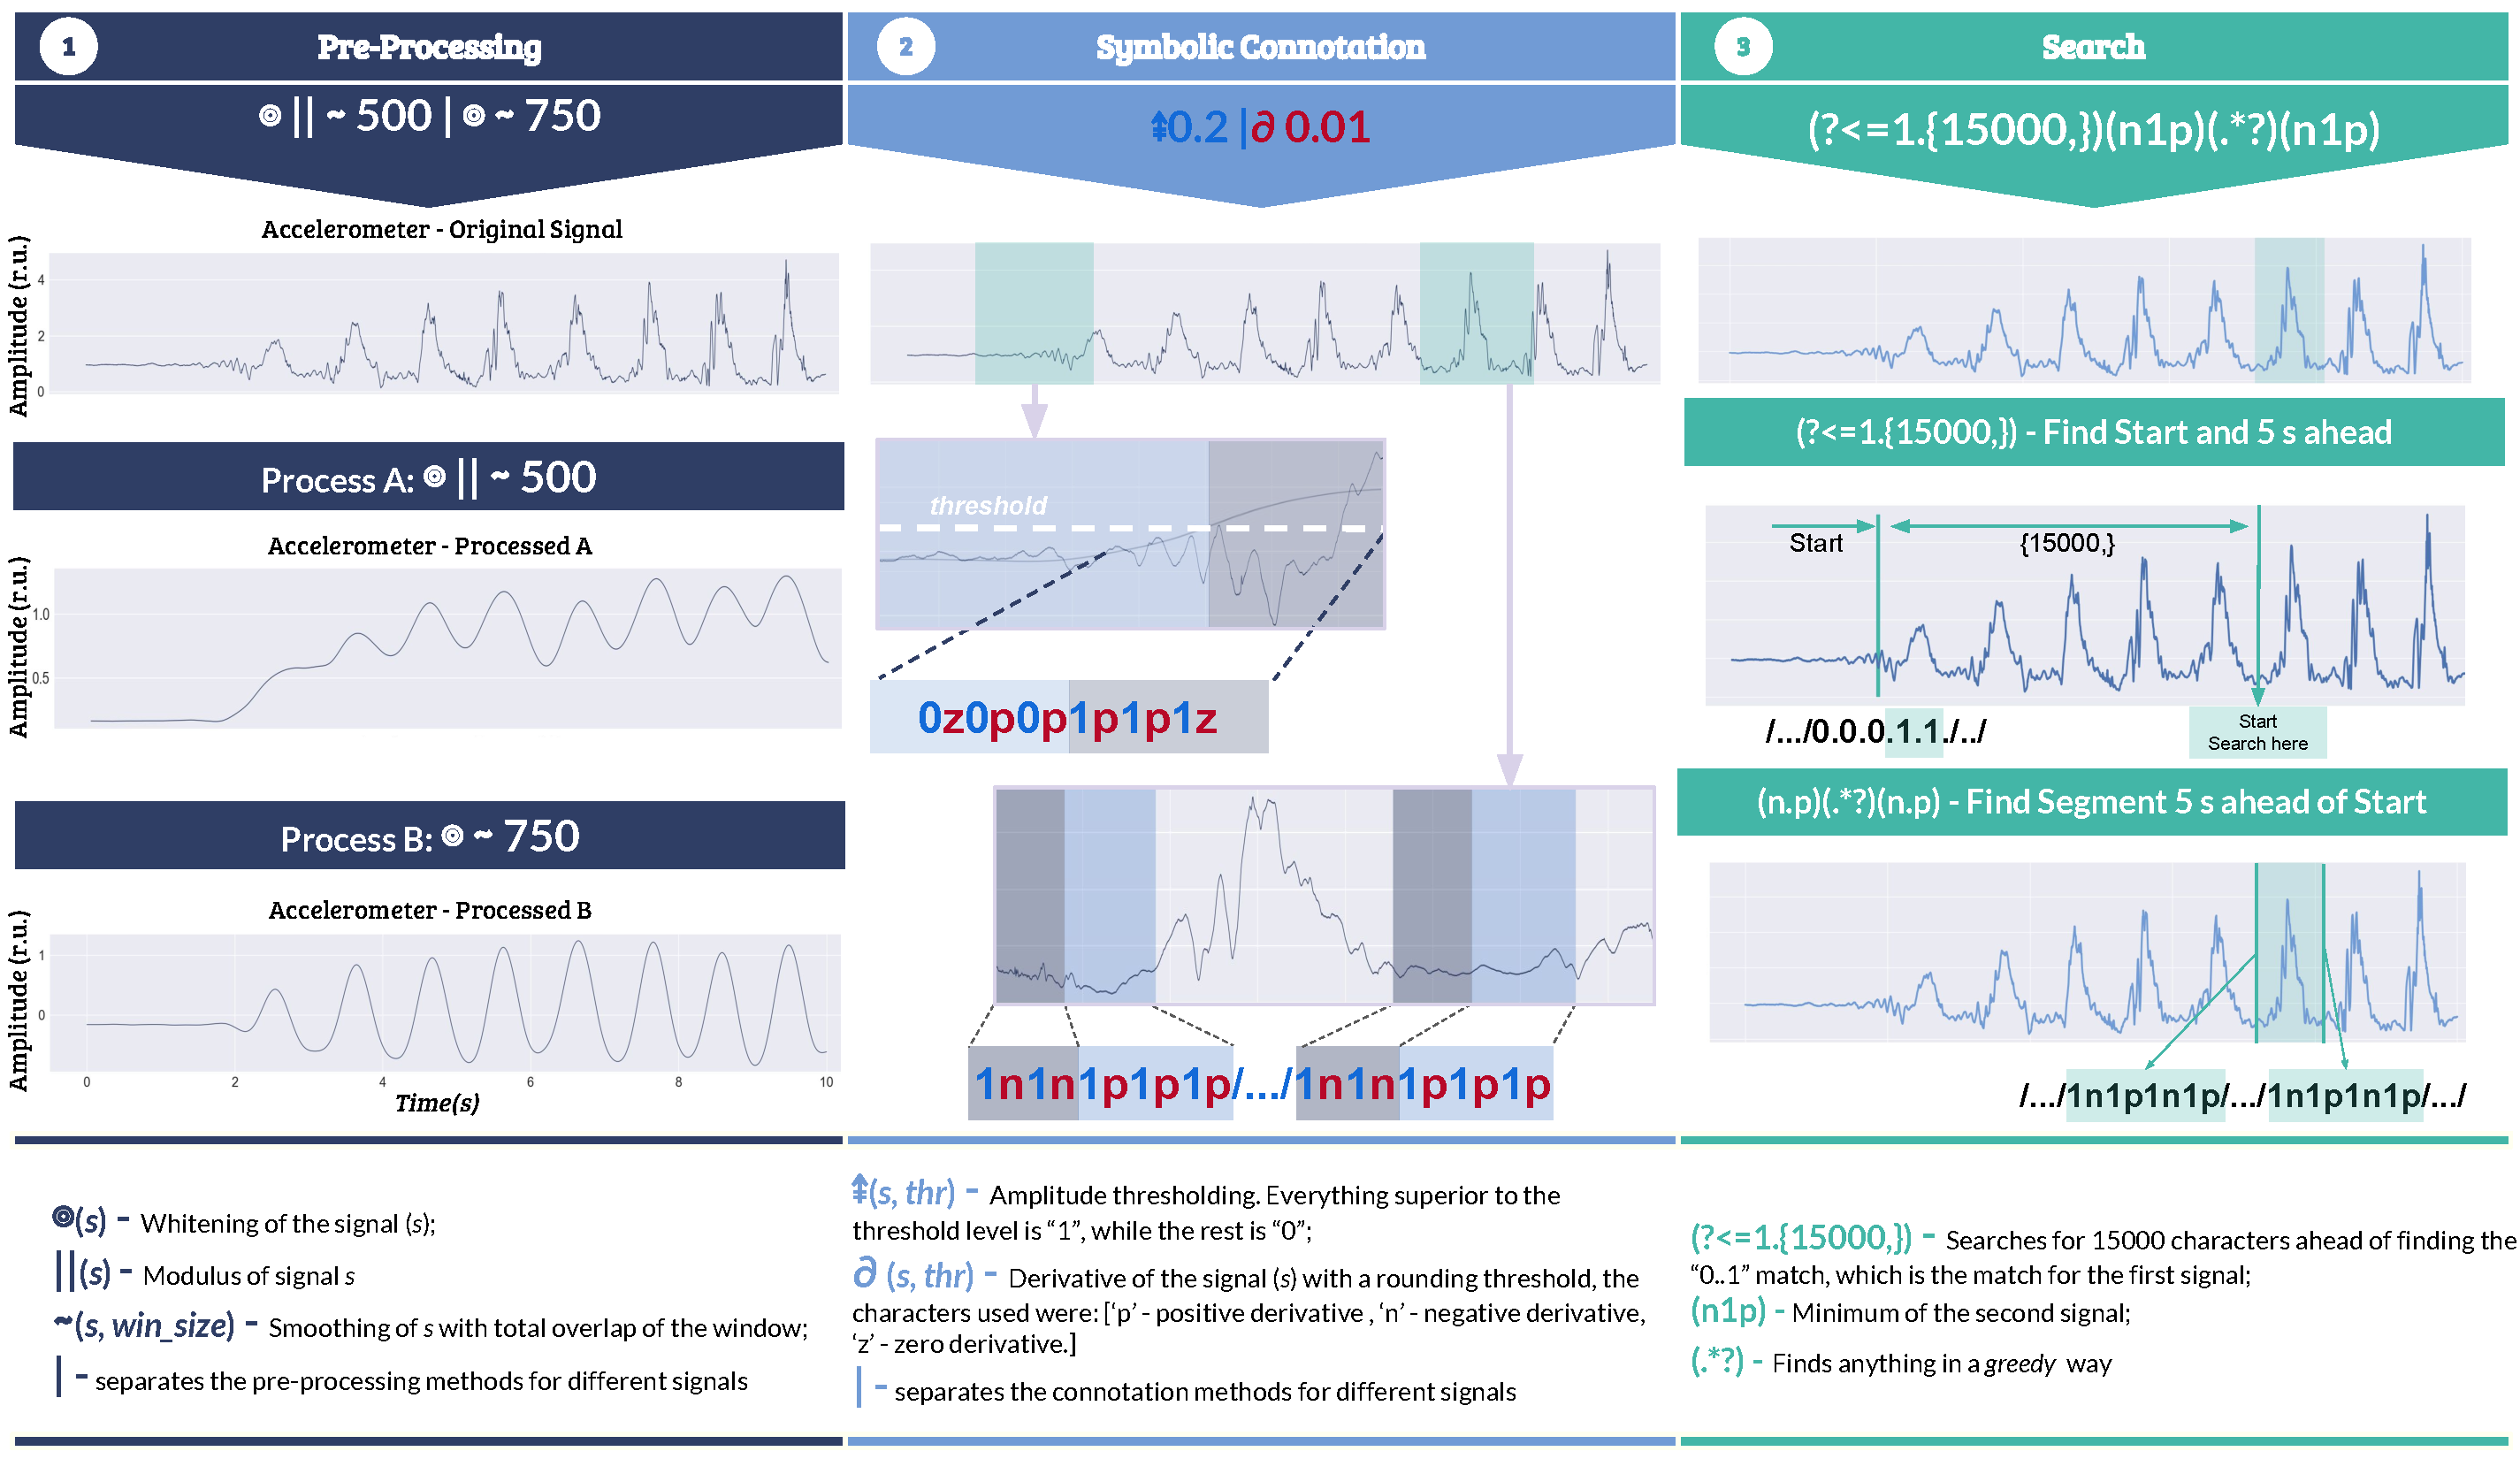
\includegraphics[width=\textwidth]{ssts_example6.pdf}
  \caption{Example 6 - Solution pipeline of Stable Lifting Detection. The operators or methods used in each step are summarized at the bottom of the figure. In the symbolic connotation step, the alternation between the methods is made with colors (Blue - \textbf{AD}, Red - \textbf{D1}). The threshold level is identified with a white dotted line. Each color band in the signal corresponds to a specific primitive. The match is highlighted with green in the "Search" step.}
  \label{fig:Hard}
\end{figure}

Fig. \ref{fig:Hard} demonstrates how the example is solved. In both pre-processing and symbolic connotation steps, a vertical bar \textbf{|} separates the methods that are applied for each representation of the same signal. The pre-processing phase uses a sequence of whitening, modulus, and smoothing of the signal for "\textit{Process A}", and a sequence of whitening and smoothing for "\textit{Process B}". The first processing sequence turns the signal similar to a plateau, in which the beginning of the activity is easily identified; whereas, in the second sequence, the signal is smoothed such that each lifting step is well defined.
\par
Regarding the symbolic connotation step, the first method AD (represented in blue) turns all sample values of the first signal that are higher than the threshold level into \texttt{1}, while the remaining samples are converted to \texttt{0}. The second set is applied to the second signal and uses the derivative of the signal D1(represented in red). Both symbolic connotations merge into a sequence of primitives, in which the first element inspects if the exercise has already started (\texttt{1.})  or not (\texttt{0.}), and the second infers the sectioning of the lifting steps, that is if the sample of the signal is increasing (\texttt{.p}), stationary (\texttt{.z}) or decreasing (\texttt{.n}).
\par
The \gls{regex} written to solve the example is \texttt{(?<=1.\{15000,\})(n1p)(.*?)}\texttt{(n1p)}. Decomposing this expression in the two steps of the example results in: (1) \texttt{(?<=1.{15000,})} and (2)\texttt{(n1p)(.*?)(n1p)}. In (1), a \textit{lookbehind} operator (recall rules from Table \ref{tab:regex} in Section \ref{subsec:regex_theory}) is used, therefore, the compiler will search ahead of the first match inside the operator, i.e., the search will match the expression "\texttt{1.\{15000,\}}" and search ahead of it. This method aims to handle the temporal dependence between events in the string, in which the number \texttt{15000} is calculated by the number of characters that correspond to 5 seconds in the string. This calculation was achieved by multiplying the sampling frequency, the number of connotations in each primitive, and the desired time, in this case: 1000 Hz, 3 connotations, and 5s, respectively.

\subsubsection{Summary of all examples}

\begin{table}
\centering
\caption{Summary of the \gls{ssts} queries used to solve the six illustrative problems.}
\resizebox{\textwidth}{!}{%
\begin{tabular}{lcccc}
\toprule
\textbf{Example} & \textbf{Fig.} & \textbf{Pre-Processing} & \textbf{Connotation} & \textbf{Search} \\
\midrule
Start of Plateau & \ref{fig:Summary2}.a & S 500 & A 0.8 D1 0.05 & \texttt{p1n}\\
End of Plateau & \ref{fig:Summary2}.a & S 500 & A 0.8 D1 0.05 & \texttt{z1n}\\
\midrule
Step Detection (Left) & \ref{fig:Summary2}.b & LP 2 Sm 50 & A 0.4 D1 0.05 & \texttt{0z0p} \\
Step Detection (Right) & \ref{fig:Summary2}.b &LP 2 Sm 50 &  A 0.3 D1 0.05 & \texttt{1z1p} \\
\midrule
Dicrotic Notch & \ref{fig:Summary2}.c & BP 1 20 & A 0.3 D1 0.01 &  \texttt{(1p).+?0} \\
\midrule
Electrocardiogram Peak Detector & \ref{fig:Summary2}.d & BP 5  50 & D1 0.01 & \texttt{pn}\\
\midrule
Straight Line Tracking & \ref{fig:Summary2}.e & none & D2 0.05 & \texttt{z*?} \\
\midrule
Stable Lifting Detection & \ref{fig:Summary2}.f & Mag Abs Sm 1000 {\large \textbf{|}} Mag Sm 750  & A 0.2 {\large \textbf{|}} A -0.2 D1 0.01 & \texttt{(?<=1.{15000,})(n.p)(.*?)(n.p)} \\
\bottomrule
\end{tabular}}
\label{tab:Summary}
\end{table}

\begin{figure}
\centering
	\begin{subfigure}{\linewidth}
    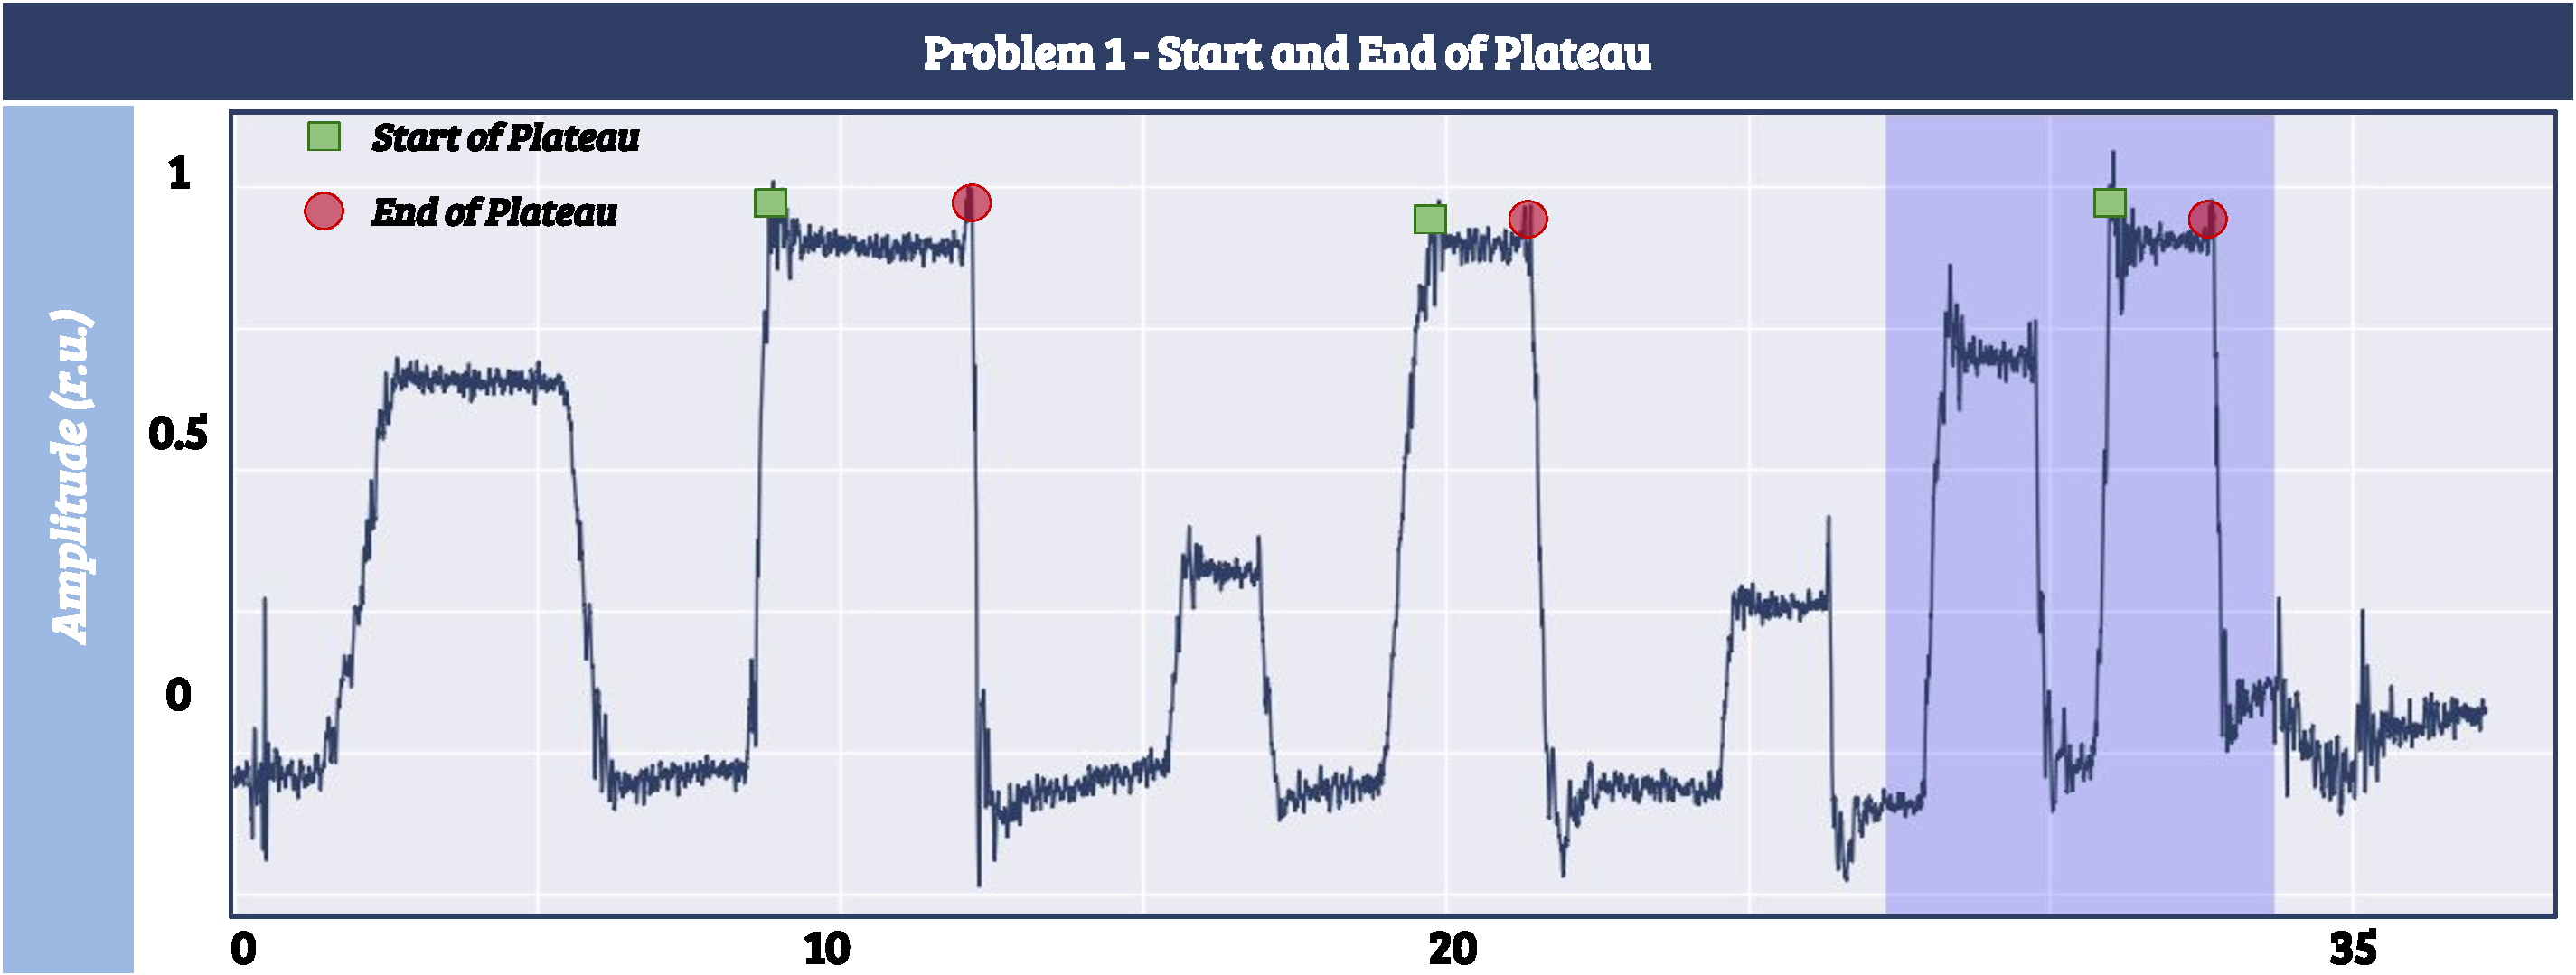
\includegraphics[width=\textwidth]{Summary_a.pdf}
    \caption{}
  	\end{subfigure}\\
	\begin{subfigure}{\linewidth}
    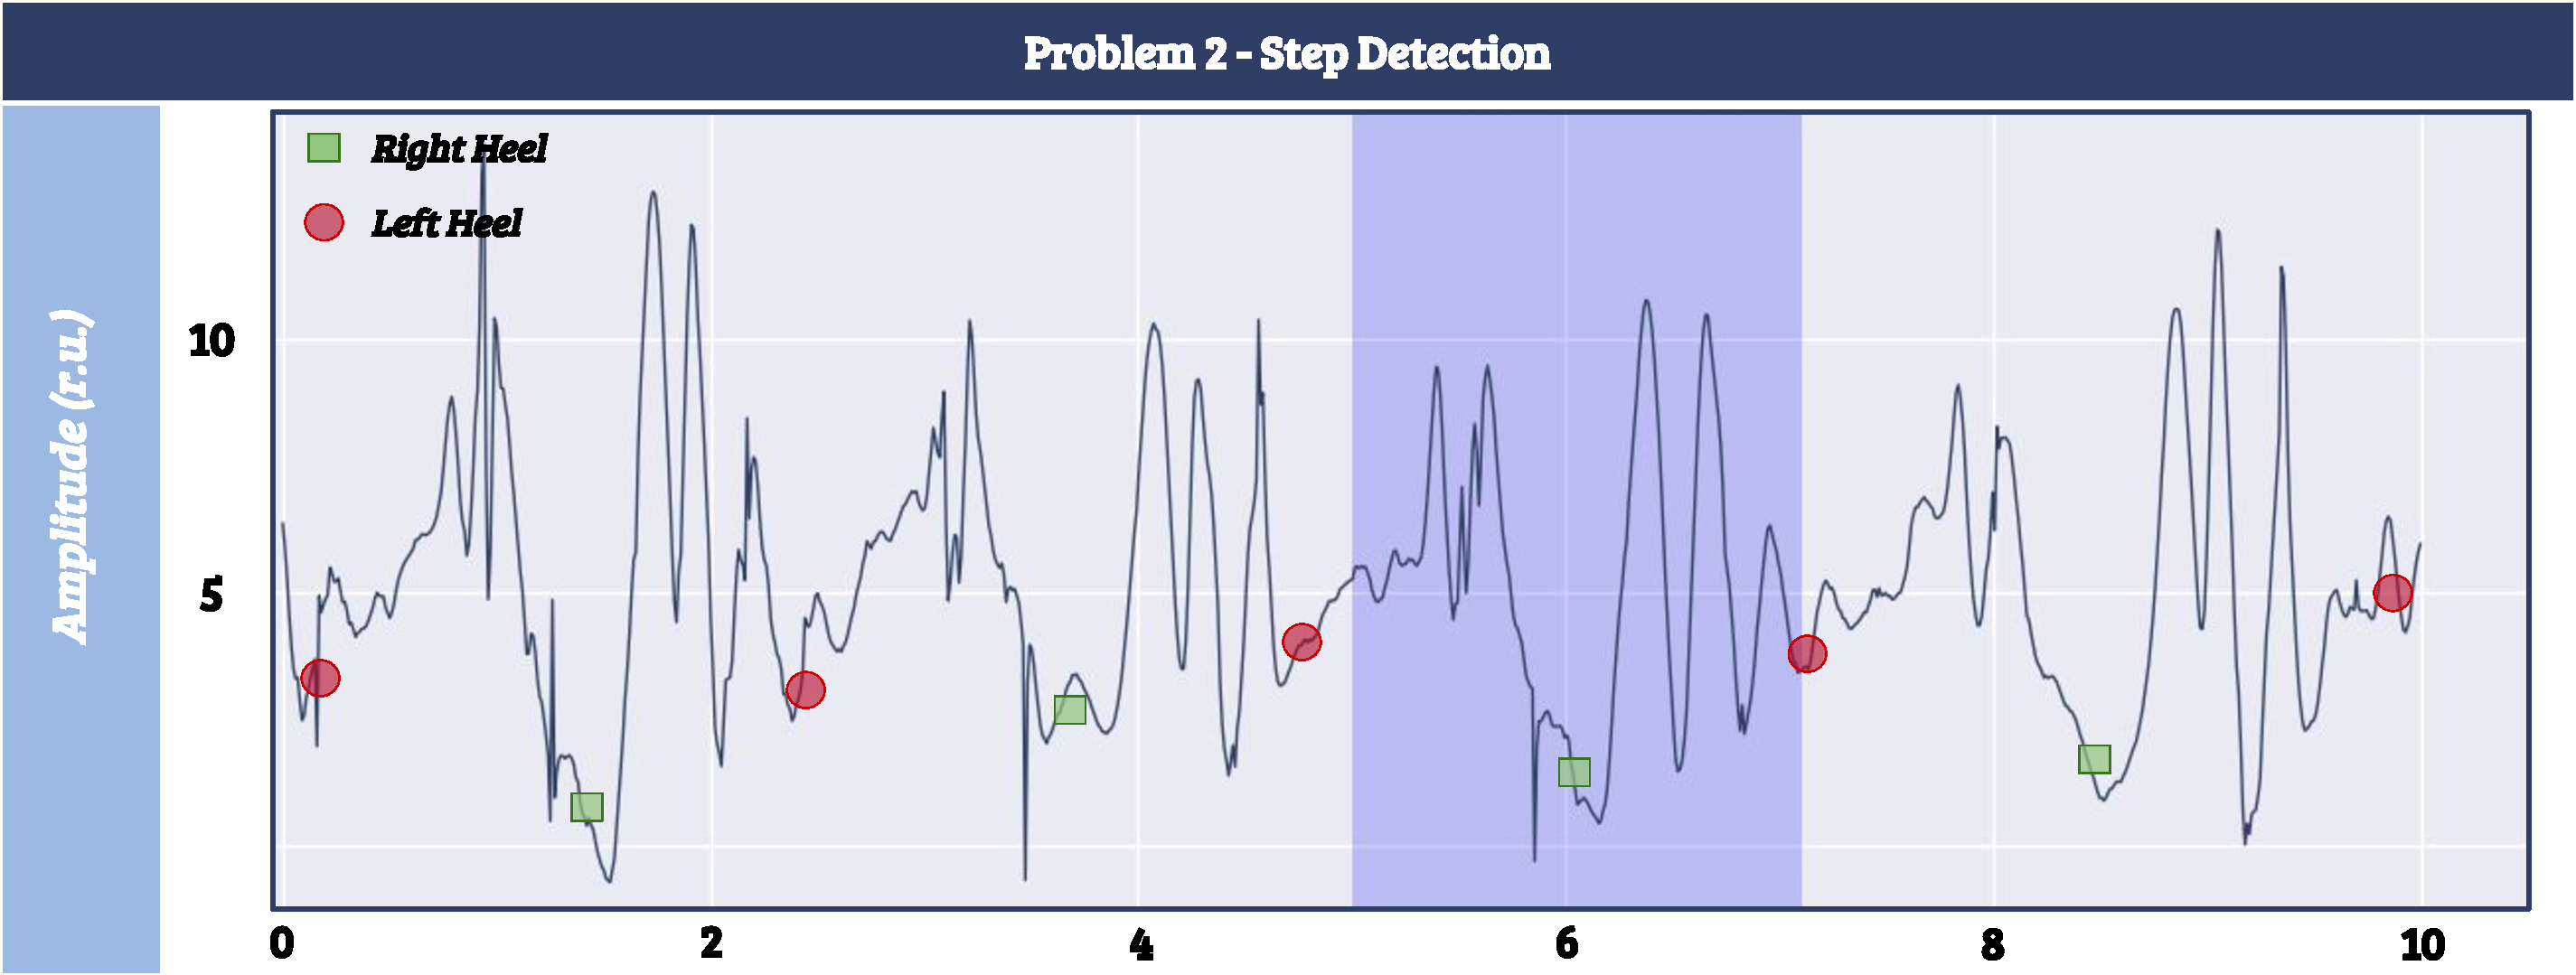
\includegraphics[width=\textwidth]{Summary_b.pdf}
    \caption{}
  	\end{subfigure}\\
    \begin{subfigure}{\textwidth}
    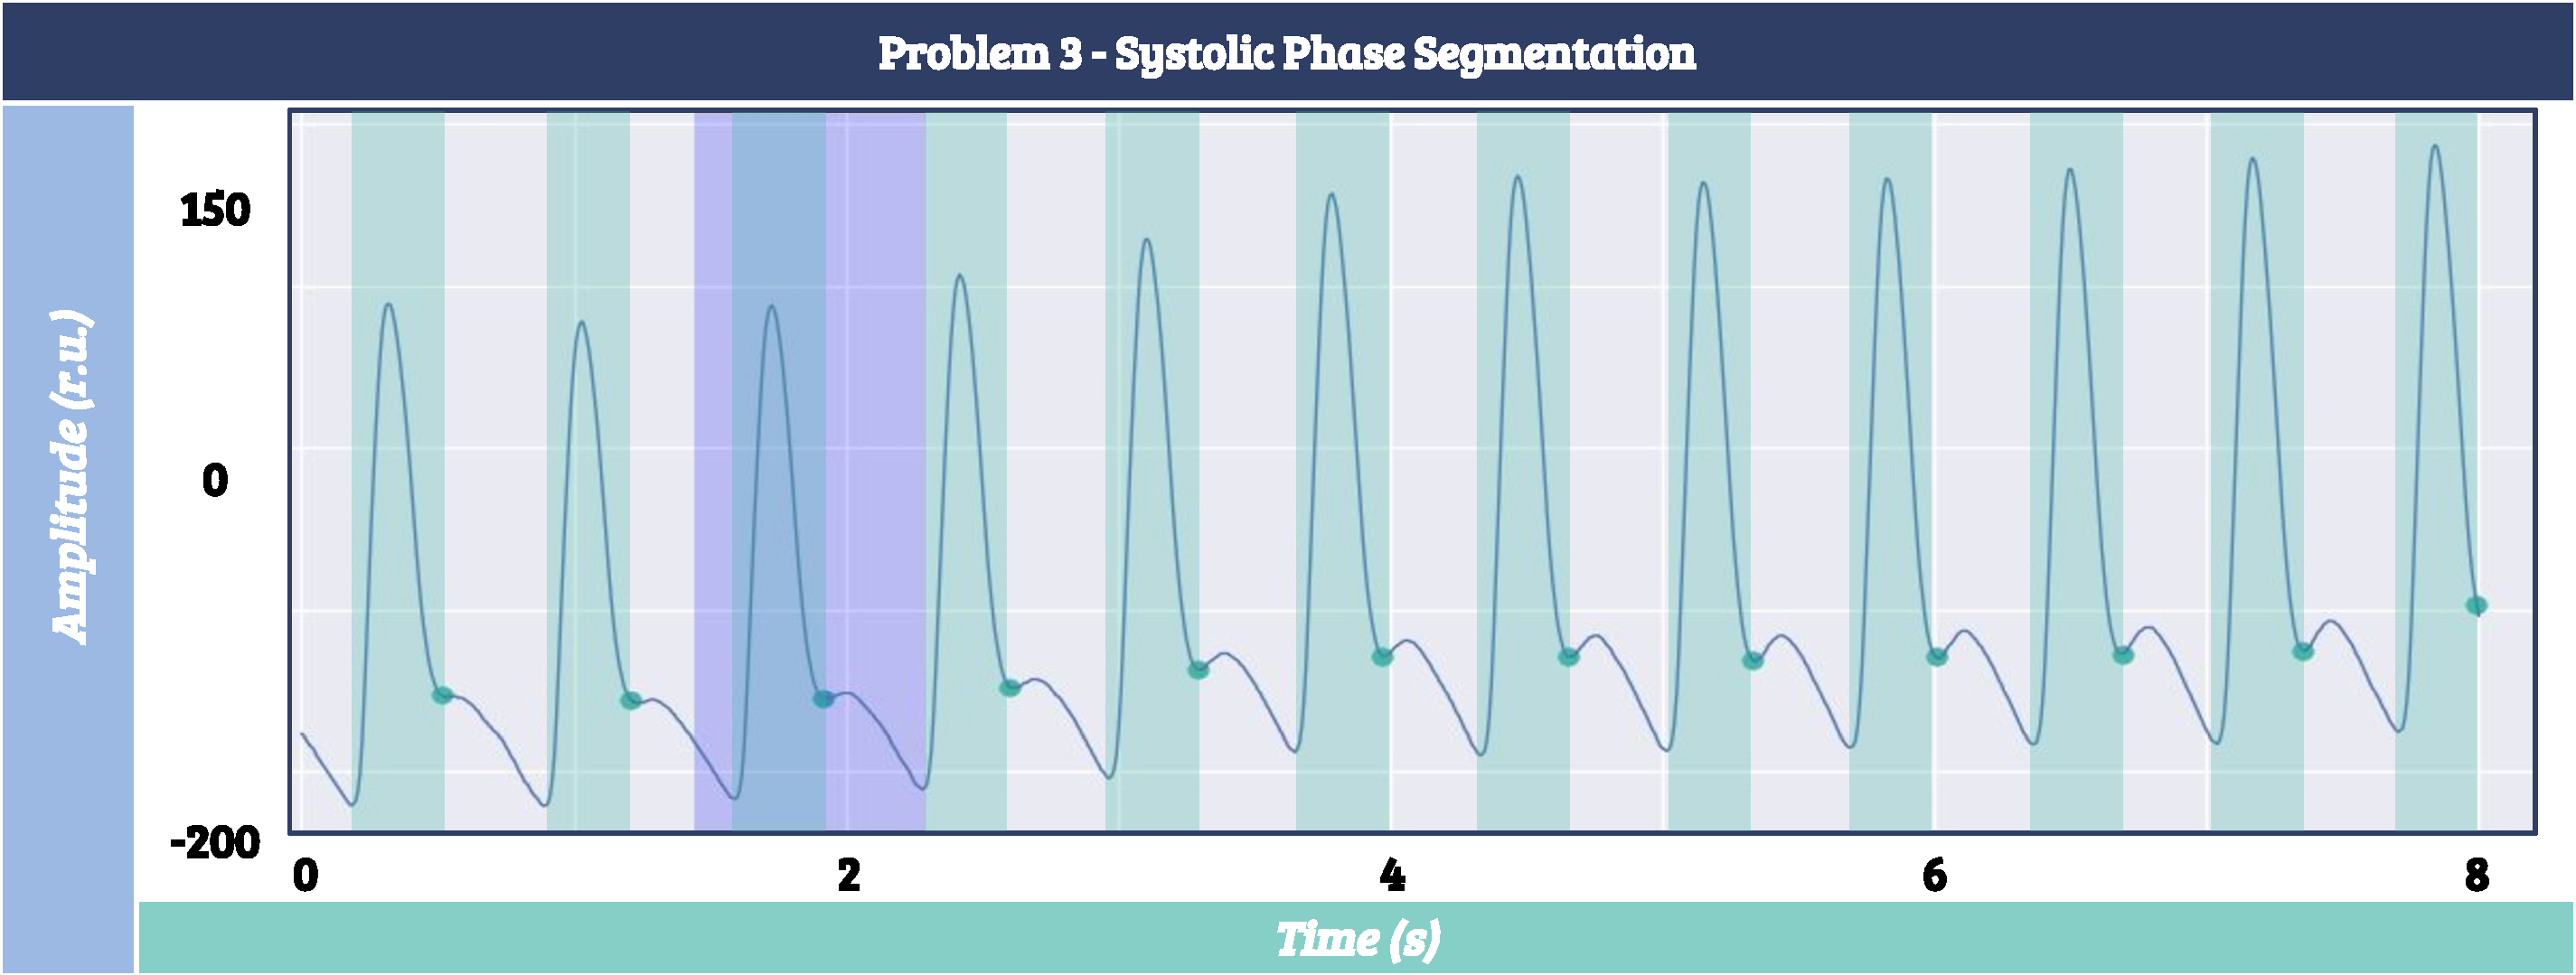
\includegraphics[width=\textwidth]{Summary_c.pdf}
    \caption{}
    \end{subfigure}	\\
     \caption{Summary of the resolution of the problems 1 (), 2 (Step Detection), and 3 (Segmentation of the systole on the \gls{abp} wave), listed in the previous Section with the \gls{ssts}.}
  \label{fig:Summary2}
\end{figure}

\begin{figure}
	\ContinuedFloat
    \begin{subfigure}{\textwidth}
    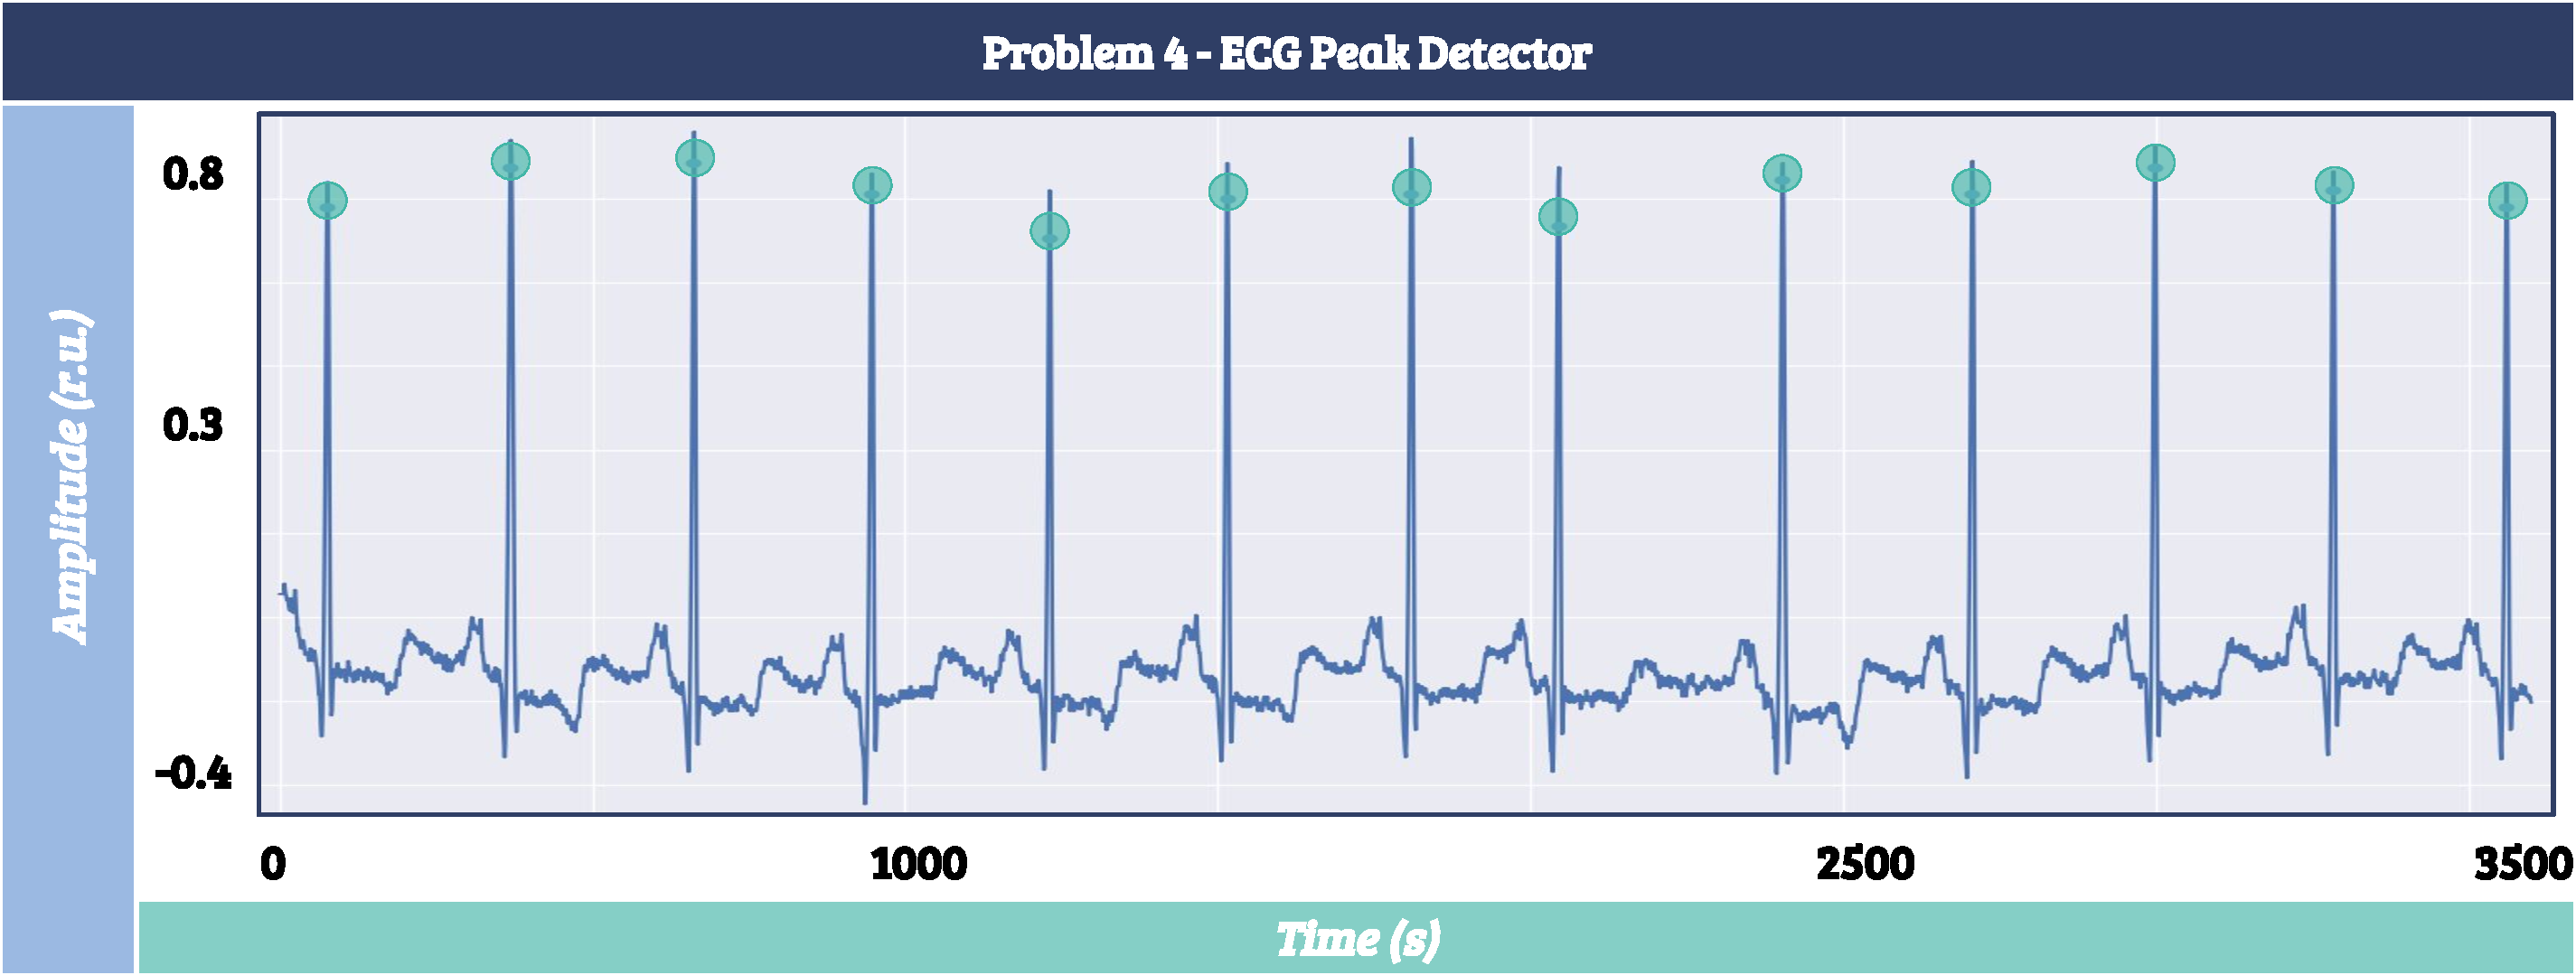
\includegraphics[width=\textwidth]{Summary_d.pdf}
    \caption{}
    \end{subfigure}\\	

    \begin{subfigure}{\textwidth}
    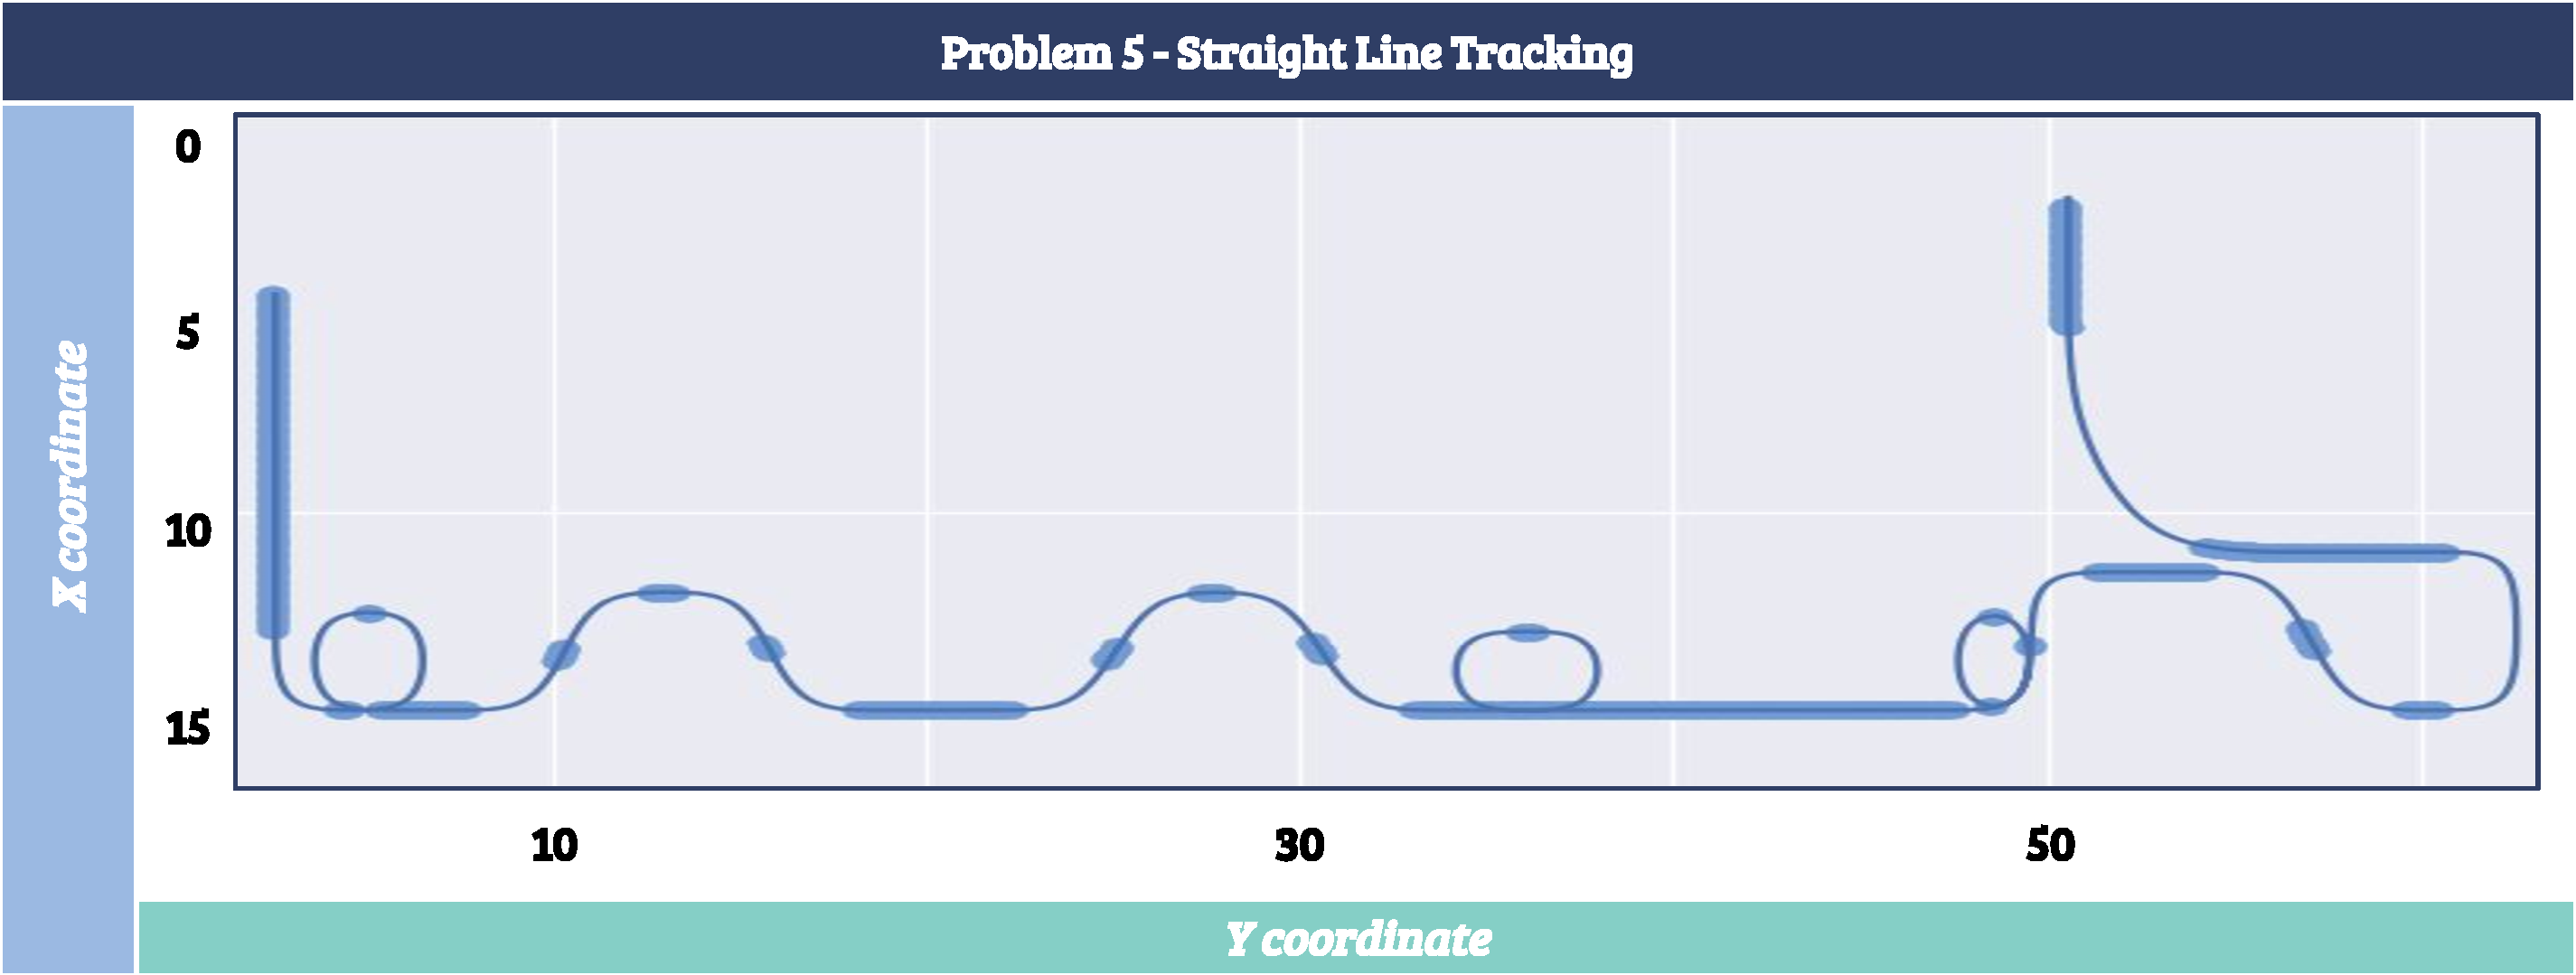
\includegraphics[width=\textwidth]{Summary_e.pdf}
    \caption{}
    \end{subfigure}	\\
    \begin{subfigure}{\textwidth}
    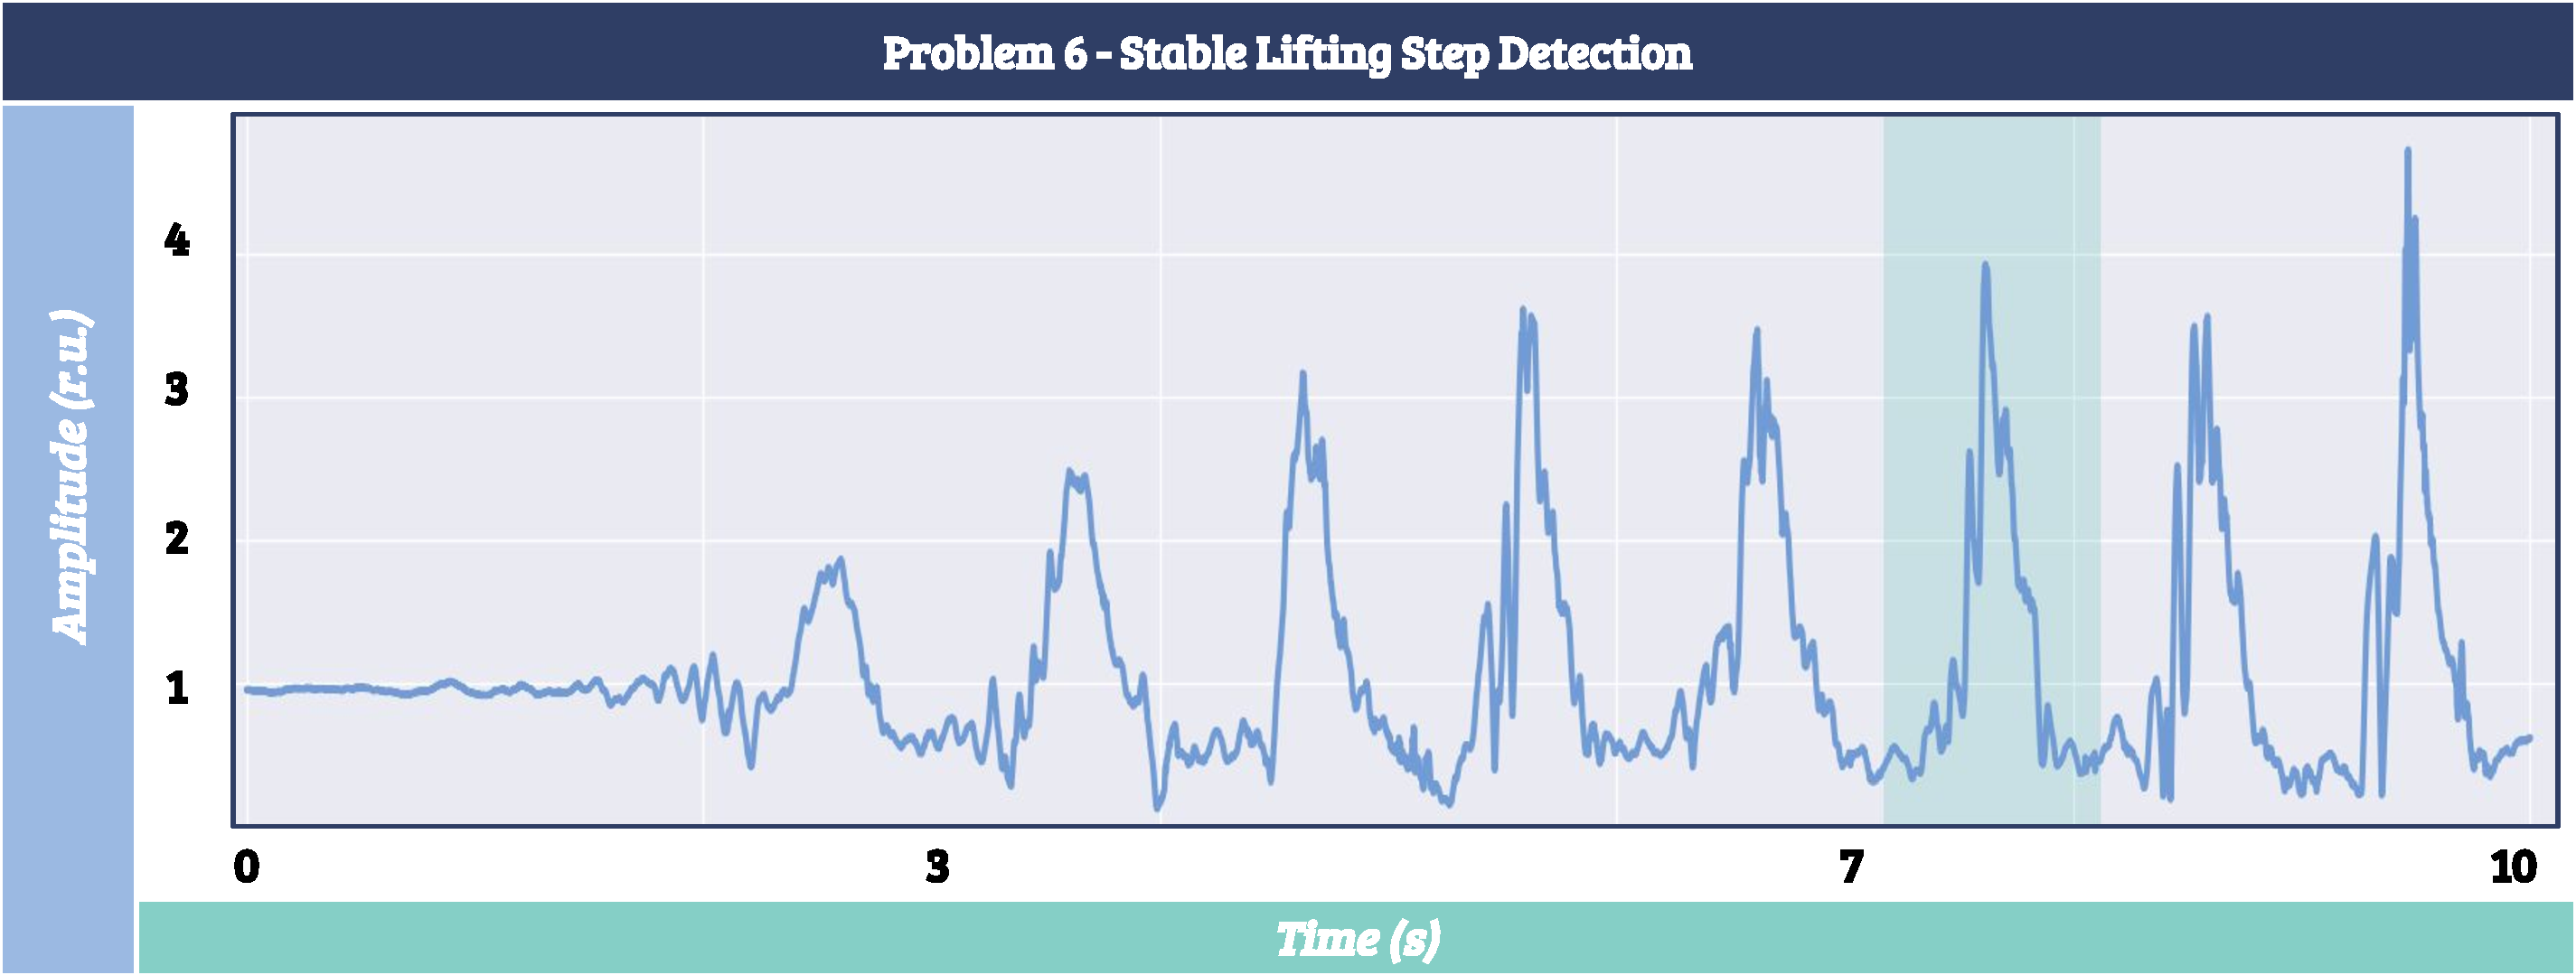
\includegraphics[width=\textwidth]{Summary_f.pdf}
    \caption{}
    \end{subfigure}\\
    \caption{(Continuation of the previous figure). Summary of the resolution of the problems 4 (Electrocardiogram peak detector), 5 (Straight line trajectory tracking), and 6 (Lifting exercise), listed in the previous Section with the \gls{ssts}.}
\end{figure}

At this point, introductory examples have been explained and can be used to understand the workability of the tool. Table \ref{tab:Summary} and Fig. \ref{fig:Summary2} summarize the example's resolution for each step of the pipeline. Additional examples are also included and can be found in the GitHub repository of the tool\footnote{\url{https://github.com/novabiosignals/SyntacticSeachOnTimeSeries}}.


\subsection{Measure of Expressiveness}

In order to evaluate parameters of expressiveness with \gls{ssts}, we evaluated the legibility and difficulty in generating the solution for the corresponding task. In the programming field, \textit{Halstead} measures are typically used for this purpose. These measures describe the complexity of the script directly from the source code, based in a set of metrics calculated with the number of distinct \gls{oprt} and \gls{oprd}, and the \gls{Toprt} and \gls{Toprd} (recall Section \ref{subsec:complex}).
\par
The complexity evaluation will be performed to compare the script generated by the \textit{classical} approach with the \textit{syntactic} approach. Concerning the \textit{classical} approach, the list of operators and operands are selected from the \textit{operator} module from python ~\cite{oprtPy}, which includes the list of arithmetic, logical, comparison, bitwise, assignment, and special operators; and, the functions that are used in the resolution process will be set as operators and their corresponding arguments as operands. For example, consider this code line written in python:

\begin{equation}
\centering
pks = peakdelta(s, delta=np.percentile(s, 70) - np.percentile(s, 30))
\end{equation}


\begin{itemize}
\item \textbf{Total List of Operators}: '\textit{peakdelta}', '\textit{percentile}', '$-$' and '\textit{percentile}'
\item \textbf{Total List of Operands}: '\textit{s}', '\textit{delta=np.percentile(s, 70) - np.percentile(s, 30)}', '\textit{s}', '\textit{70}', '\textit{s}', '\textit{np.percentile(s,30)}', '\textit{np.percentile(s,70)}' and '\textit{30}'
\item \textbf{List of Distinct Operators}: '\textit{peakdelta}', '\textit{percentile}' and '$-$'
\item \textbf{List of Distinct Operands}: '\textit{s}', '\textit{delta=np.percentile(s, 70) - np.percentile(s, 30)}', '\textit{np.percentile(s, 70)}', '\textit{np.percentile(s, 30)}',  '\textit{70}' and '\textit{30}'
\end{itemize}

In the second case, both \textbf{connotation} step and \textbf{search} procedure will be inspected for the \textbf{difficulty} measures. Regarding the \textbf{connotation} step, the evaluation will be made similarly to the previous method for inspecting functions, in which the function is set as an operator and its corresponding arguments as operands. For the \textbf{search} procedure, the set of instructions typically used in \gls{regex} (except the "." character) is defined as operators\cite{regex}. These can be revisited in the second section. The remaining characters of the \gls{regex} string, except the parenthesis, will be set as operands. In this are included the "." operator that matches any character, and the "\textbackslash d" and "\textbackslash w" that matches all digits and alphabetical characters respectively. Regarding the parenthesis, when occurring ("\{\}" or "[]"), will be set as one operator. For example:\\

{\centering
\textbf{$Connotation: $} $Sm$ 500  $A$ 0.8 $D1$ 0.05\\
\textbf{$Search: $} \texttt{(z1n).*?}\\ }

\begin{itemize}
\item \textbf{Total List of Operators}: '$Sm$', '$A$', '$D1$', '( )' and '\textit{*?}'
\item \textbf{Total List of Operands}: '\textit{500}', '\textit{0.8}', '\textit{0.05}', '\textit{z}', '\textit{1}', '\textit{n}' and '\textit{.}'
\item \textbf{List of Distinct Operators}: '$Sm$', '$A$', '$D1$', '( )' and '\textit{*?}'
\item \textbf{List of Distinct Operands}: '\textit{500}', '\textit{0.8}', '\textit{0.05}', '\textit{z}', '\textit{1}', '\textit{n}' and '\textit{.}'
\end{itemize}


\begin{table}[h!]
\centering
\caption{Evaluation of the complexity in the resolution of examples with the \textit{syntactic} approach and with the \textit{classical} approach. Voc - Vocabulary, Lgth - Length, CL - Calculated Length, V - volume, D - difficulty, E - effort.}
\label{tab:halstead}
   \small
    \setlength{\tabcolsep}{3pt}
    \renewcommand{\arraystretch}{0.8}
    \resizebox{\textwidth}{!}{%
    \begin{tabular}{cl cccccc cccccc}
    	
        \toprule[0.5mm]\\
        
        \multirow{2}{*}{Example} & & \multicolumn{6}{c}{Syntactic Resolution} & \multicolumn{6}{c}{Classical Resolution}\\
        
        \cmidrule[0.2mm](lr){3-8} \cmidrule[0.2mm](lr){9-14} & & \textit{\textbf{Voc}} & \textit{\textbf{Lgth}} & \textit{\textbf{CL}} & \textit{\textbf{V}} & \textit{\textbf{D}} & \textit{\textbf{E}} &
        \textit{\textbf{Voc}} & \textit{\textbf{Lgth}} & \textit{\textbf{CL}} & \textit{\textbf{V}} & \textit{\textbf{D}} & \textit{\textbf{E}} \\      
        
        \midrule[0.3mm]\\
        
        Start/End of Plateau & & 5.0 & 5.0 & 8.0 & 11.6 & 1.5 & \textbf{17.41} & \maxf{12.0} & \maxf{13.0} & \maxf{33.3} & \maxf{46.6} & \maxf{2.5} & \maxf{\textbf{116.5}}\\
         
        \midrule[0.3mm]\\
        
        Step Detection (Left \& Right Heel) & & 5.0 & 6.0 & 8.0 & 13.9 & 1.75 & \textbf{24.38} & \maxf{19.0} & \maxf{22.0} & \maxf{63.6} & \maxf{93.5} &\maxf{ 4.2} &  \maxf{\textbf{388.2}}\\
        
        \midrule[0.3mm]\\
        
        Dicrotic Notch & & 7.0 & 7.0 & 13.6 & 19.7 & 2.0 & \textbf{39.3} & \maxf{21.0} & \maxf{25.0} & \maxf{73.0} & \maxf{109.8} & \maxf{4.7} & \maxf{\textbf{517.7}}\\
        
        \midrule[0.3mm]\\
        
        Electrocardiogram Peak Detection & & 2.0 & 2.0 & 2.0 & 2.0 & 1.0 & \textbf{2.0} & \maxf{9.0} & \maxf{12.0} & \maxf{20.3} & \maxf{38.0} & \maxf{3.0} & \maxf{\textbf{114.0}}\\
        
        \midrule[0.3mm]\\
        
        Straight Line Tracking & & 2.0 & 2.0 & 0.0 & 2.0 & 1.5 & \textbf{3.0} & \maxf{25.0} &\maxf{33.0}& \maxf{93.5} & \maxf{153.2} & \maxf{5.3} & \maxf{\textbf{811.3}}\\
        
        \midrule[0.3mm]\\
        
        Stable Lifting Detection & & 10.0 & 18.0 & 24.4 & 59.8 &3.6 & \textbf{217.8} & \maxf{22.0} & \maxf{23.0} & \maxf{77.3} & \maxf{102.6} & \maxf{5.0} & \maxf{\textbf{512.8}}\\

        \bottomrule[0.5mm] \\
        
    \end{tabular}}
\end{table}

Table \ref{tab:halstead} presents the performance measurements for both methods of solving the demonstrated examples. For the evaluation, the pre-processing step was omitted, which means that only the \gls{regex} is used to compute the difficulty measures for the \textit{syntactic} approach, and only the script after the pre-processing steps is used to compute the difficulty measures for the \textit{classical} approach.

\subsection{Discussion}
\label{sec:discussion_ssts}

The previous section demonstrated the potential of the proposed framework in delivering a more expressive methodology of solving query search tasks in time series. For the complete group of examples presented, all the steps involved were written in a symbolic manner. This fact eased the way in which time series are interpreted and how the final search is achieved.
\par
The results from the \textit{Halstead} measurements summarized in Table \ref{tab:halstead} demonstrate that, in general, the complexity is decreased using the \gls{ssts} approach in comparison with the classical solution. In the circumstances in which the difference is not significant, such as the \textit{Example 6} (Stable Lifting Detection), the complexity measurements increase significantly. This fact suggests that for more complicated problems, the complexity of the \gls{regex} increases.

\subsubsection{Symbolic series generation}
\label{sucsec:string_generation}

Overall, most of the symbolic series that are generated by the symbolic connotation step are simple to read and interpret. Nevertheless, the complexity of the series linearly increases with the number of operators used to perform the symbolic connotation. Consequently, for problems that have inherent and higher complexity, and require the use of several connotation groups, it is expected that the legibility of the symbolic sequence will also be reduced. \textit{Example 6} constitutes an example of the mentioned drawback, as it involves two distinct resolution steps and revealed to be much more complicated to understand without any previous insights.

\subsubsection{Required background knowledge}
\label{sucsec:required_knowledge}

Each step of the \gls{ssts} pipeline has an important role in solving the examples, especially the two initial steps (pre-processing and symbolic connotation). Both steps aim to simplify the signal, such that the search procedure can be composed as easily as possible. This approach aims to prepare the signal so that a sequence of symbols can be used to simplify the search step. Therefore, choosing an adequate set of pre-processing methods and proper coordination with the symbolic connotation methods will reduce the search task complexity, both in the writing and interpretation processes.
\par
\gls{ssts} users' should have background knowledge in both signal processing techniques and \gls{regex}. In fact, without prior consolidation of these topics, the user might have an additional effort in generating a solution to solve the required problems. Firstly, for circumstances in which the user experiences difficulty in using such methods, the pre-processing and the symbolic connotation steps will not be so intuitive. Secondly, for in case the user is not familiarized with \gls{regex}, it will be hard to generate appropriate expressions to search for patterns on the symbolic time series, especially for more difficult problems, which require the use of advanced operators.
\par
As a future objective, we expect to increase the expressiveness of the tool and reduce the required knowledge to accomplish signal processing tasks and \gls{regex} queries. In order to achieve a more simplified pipeline, a set of pre-processing and symbolic connotation templates for specific types of data (e.g. electrocardiogram) should be available to the user. Furthermore, the search step could be also simplified using meta-\gls{regex}. In addition, a flexibility in the search process should be considered. \gls{regex} are powerful tools, but lack flexibility, in the sense that the pattern is or not matched by the \gls{regex}. Instead, a score function based on the query should be considered to make a flexible search and provide an error margin to the user.\\\\

We expect \gls{ssts} to have a broad range of applications that can extend to the query-based search problematic. Other topics in time series data mining, such as \textit{signal generation}, \textit{segmentation}, \textit{feature extraction}, \textit{labelling} and \textit{classification}, could benefit from this reasoning. In this thesis, only the classification topic was explored. In the next Section, we present our results.

\section{Time Series Classification with HeaRTS}

In this section, the performance of \gls{hearts} is evaluated in the time series classification task by being applied to the \textit{UCR time series classification benchmark} and compared with the traditional 1-NN \gls{ed}. As was mentioned on Chapter \ref{sec:hearts}, this process can be performed in multiple ways, namely with the combination of a \textit{Baysian} or \gls{svm} classifiers with either a \gls{bow} or a \gls{tfidf} model. These combinations were also compared. This evaluation will help us answer if it is possible to use a text-based representation of time series with words extracted by \gls{ssts} queries with a traditional text-mining strategy.

In addition to these experiments, we performed an individual analysis of several use-cases to understand how to extract meaningful explanation about differences between signals based on this linguistic translation. This study should tell us if the words extracted are valuable to highlight the \textit{subsequences} that are most relevant to distinguish the time series from one class in regard to all the others. 

\subsection{Classification Performance}

Figure \ref{fig:distribution_dendogram} showed us how vectorized documents can be compared with the cosine distance to distinguish time series. Simply by using part of the \gls{ssts} queries, it is possible to generate \gls{tfidf} weights that are differently distributed based on ordered words on a time series document. Of course, the \textit{Trace} dataset used for this example is a simple dataset, with simple dynamics, but still challenging to classify well with the 1-NN \gls{ed} (only 76\% of accuracy). Therefore, to validate the ability of the proposed method to perform time series classification, it was computed on all available datasets of the UCR Benchmark and its performance compared with the standard 1-NN \gls{ed}. In order to perform this evaluation, we followed the indications provided by the authors of the dataset \cite{ucr}. As recommended, we used the reference \textit{train/test} split, and performed a cross-validation for hyperparameter tuning with the standard \textit{train} set.

As mentioned on Section \ref{sec:ssts}, the method translates the time series into text with \gls{ssts} queries from Table \ref{tab:ssts_queries}. These have pre-processing, connotation, and search steps. For each step, relevant parameters are necessary depending on the queries used. For this experiment, we used as pre-processing a simple smoothing, which requires a \textit{window size} ($w_s$). The derivative connotation steps also required a specific threshold ($thr$). In addition, the \gls{bow} and \gls{tfidf} models can be built with different \textit{n-gram} sizes:

\begin{equation}
\begin{gathered}
w_s \in [1, 10, 25, 50, 100, 250]\\
thr \in [0.001, 0.01, 0.05, 0.1]\\
n-gram \in [1, 2, 3, 4, 5, 6]\\
\end{gathered}
\end{equation}

The cross-validation step for hyperparameter tuning was performed differently depending on the size of the dataset. For datasets with more than one hundred signals, we performed a 10 fold stratified (K-SF) cross validation, while on datasets with less than one hundred signals, a leave one out (LOO) cross validation was performed instead. The \textit{K-SF} cross-validation step was chosen on larger datasets because of its higher computational speed performance in comparison with the \textit{LOO}. In shorter datasets, using the \textit{K-SF} would reduce the training set size too much and with unbalanced training samples for certain classes, and, as recommended by \cite{ucr}, we used the \textit{LOO} instead. We then selected the parameters set with best average cross-validation F1-scores for each dataset and performed the validation on the \textit{test} set, to which the model was \textit{blind} to.

We performed this experiment with several strategies and combinations, namely: \gls{bow} with Bayesian Classifier (BoW+NB), \gls{bow} with \gls{svm} (BoW+SVM), \gls{tfidf} with Bayesian Classifier (TF-IDF+NB) and \gls{tfidf} with \gls{svm}. The summary of the performance is presented in Figure \ref{fig:critical_distances}.

\begin{figure}
    \centering
    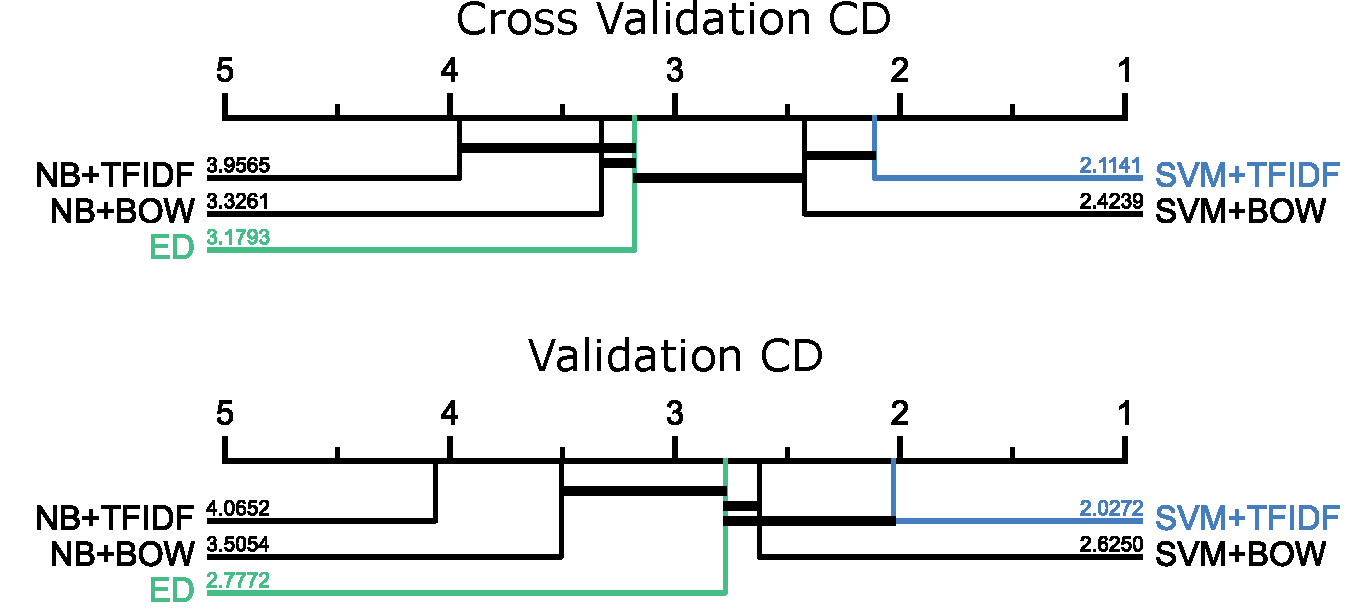
\includegraphics[width=\linewidth]{hearts_CriticalDistanceDiagram.pdf}
    \caption{Critical distance diagram for the methods that rely in a textual representation of the time series (\gls{bow} and \gls{tfidf}) and euclidean distance for: \textbf{Top)} the cross-validation stage; and \textbf{Bottom)} the validation step. The closer to \textbf{1} is the method, the better it is. Thick lines between methods indicate that these have not a significant performance difference.}
    \label{fig:critical_distances}
\end{figure}

The performance was measured for both the cross-validation step and the validation step. The overall results can be found in Appendix \ref{appendix:tables_detailed}, Section \ref{subsec:hearts_all_accuracies}. As can be seen, the strategies that rely on a \gls{svm} classifier are more robust. The \gls{tfidf} turns out to not be reliable when used with the \gls{nb} classifier, which has much better results when the \gls{bow} model is used instead. On the other end, the \gls{tfidf} model works well with the linear \gls{svm} classifier, being the method with highest average accuracy.

\begin{figure}
    \centering
    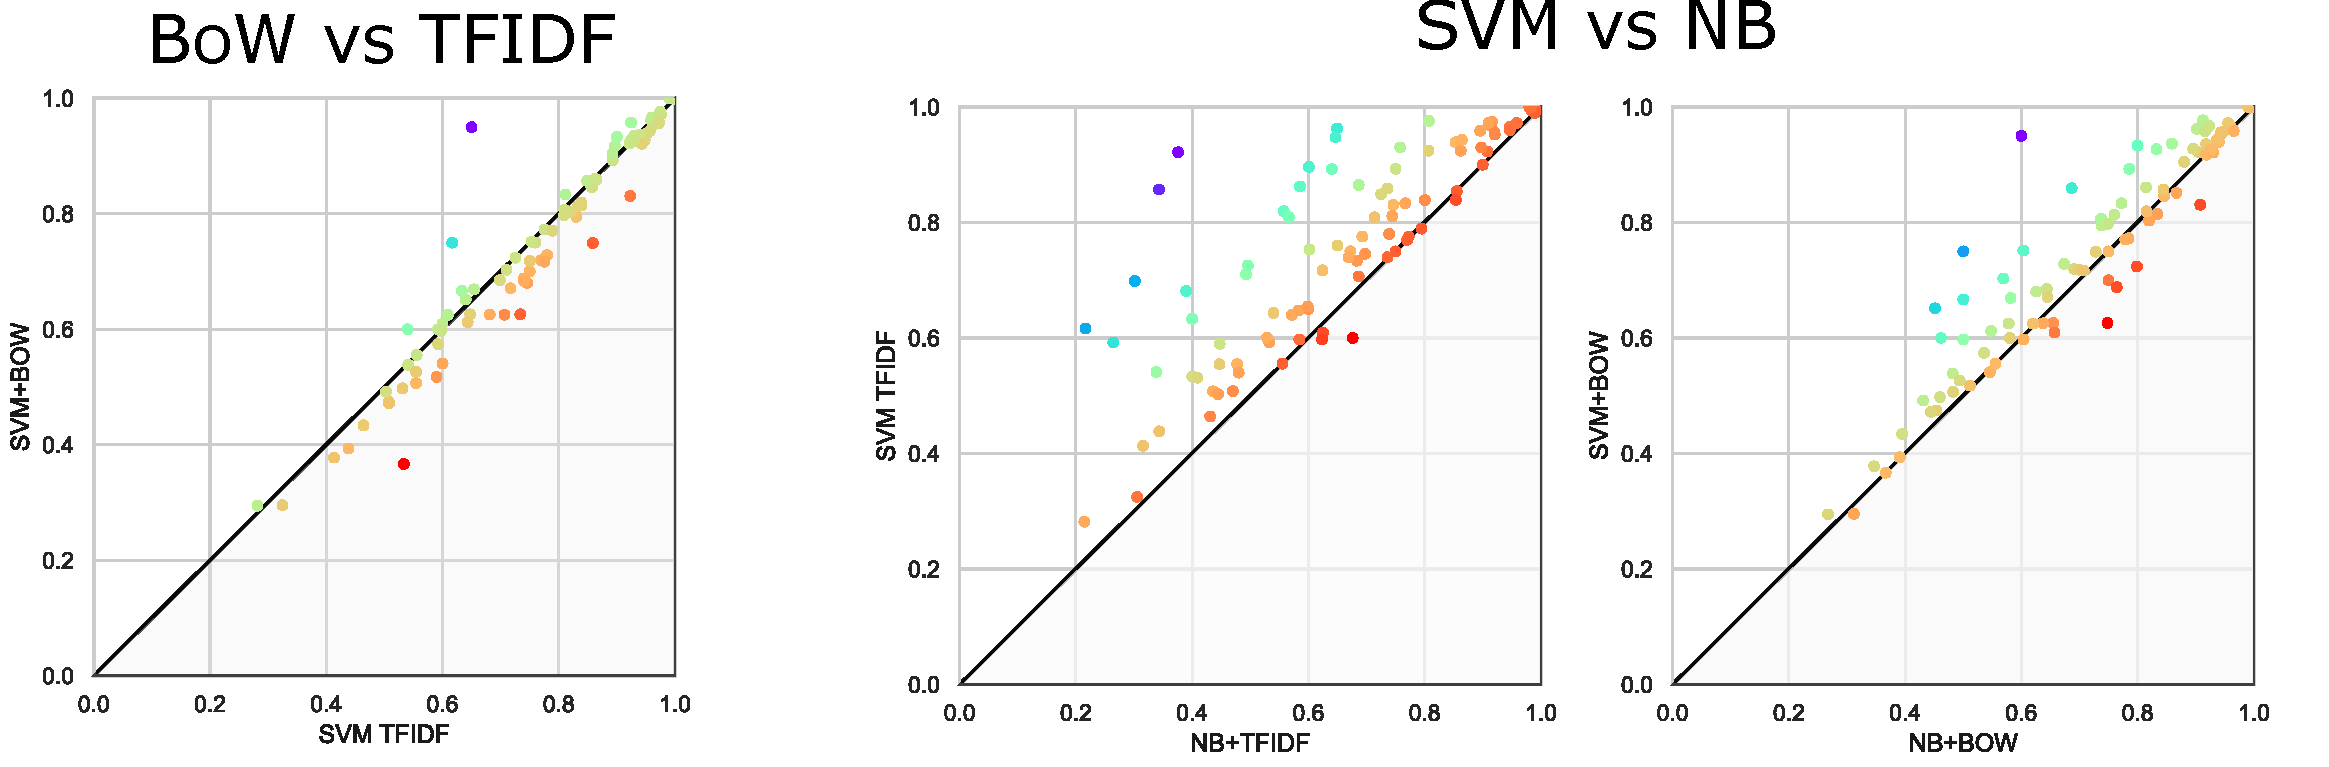
\includegraphics[width=0.95\linewidth]{hearts_methods_comparisons.pdf}
    \caption{right) Classification accuracies for the Bag of Synthatic Patterns in comparison with the euclidean distance combined with 1-NN classifier (1-NN ED) with standard train and test; left) with a 10 fold cross validation.}
    \label{fig:comparison_2}
\end{figure}

Figure \ref{fig:critical_distances} also shows that there is a significant distance in performance between the TFIDF+SVM model in comparison with the 1-NN \gls{ed} method during the cross-validation step. However this significance is not as expressive in the validation step. All these remarks are also highlighted in Figure \ref{fig:comparison_2}, where both models (\gls{bow} and \gls{tfidf}) and classifiers (\gls{svm} and \gls{nb}) were compared (left and right, respectively).  When comparing both models (\gls{bow} and \gls{tfidf}), we see that the best performances are similar, with a slightly better accuracy achieved with the \gls{tfidf} model. In regard to using the \gls{svm} or the \gls{nb}, as mentioned previously, better results are achieve when using the \gls{svm} classifier, for both models (TFIDF on the left, and BOW on the right, of the right graphs).

We are now in position to compare the best text-based method (\gls{hearts}) with the 1-NN \gls{ed} classifier. This result is presented in Figure \ref{fig:comparison_2}, for both cross-validation and test steps.

\begin{figure}
    \centering
    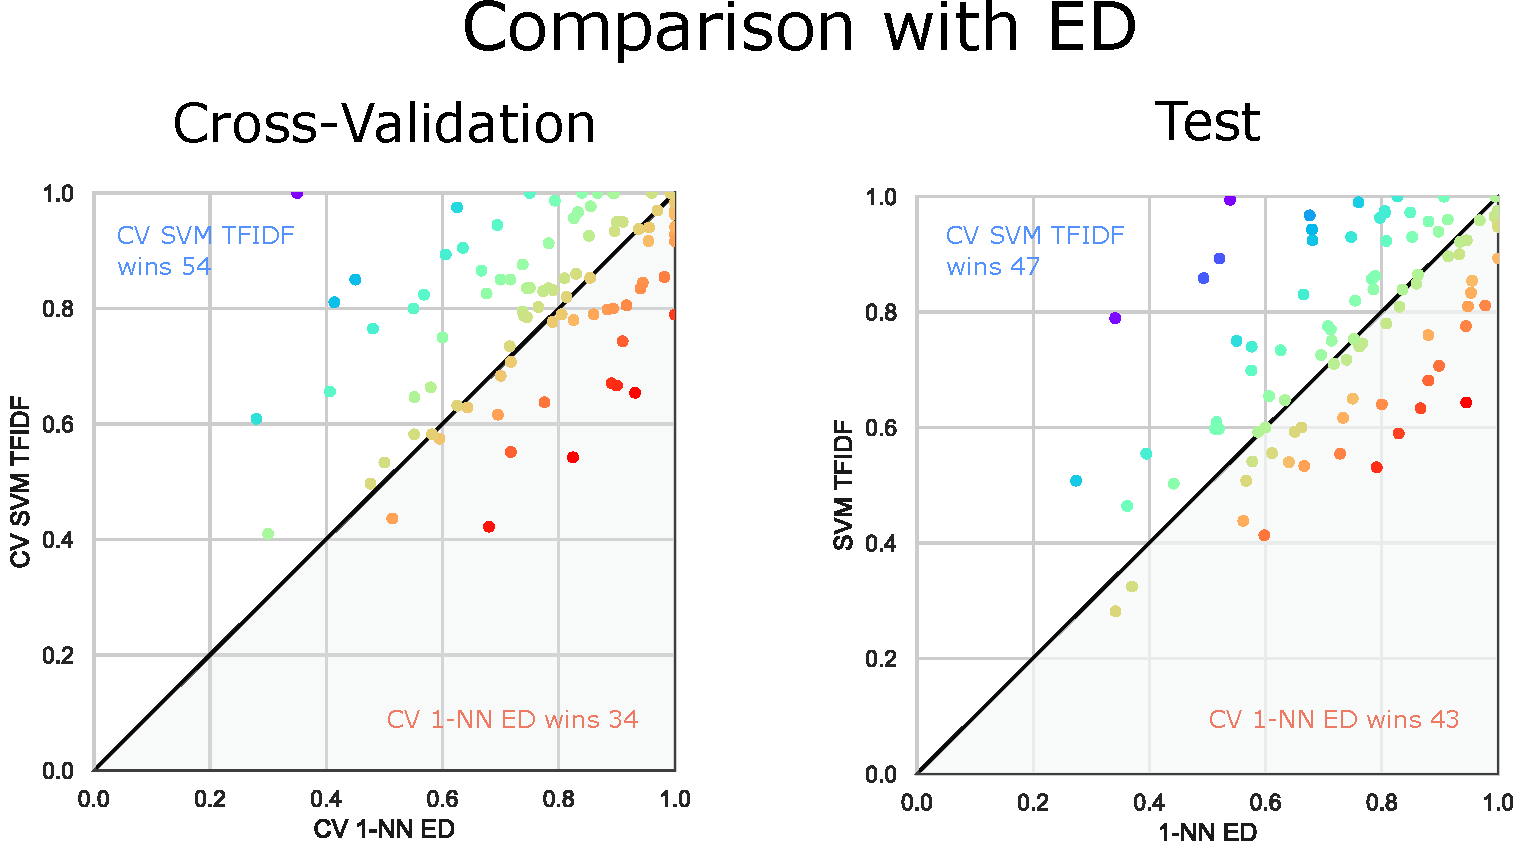
\includegraphics[width=0.95\linewidth]{hearts_comparison_with_ED_MAIN.pdf}
    \caption{right) Classification accuracies for the Bag of Synthatic Patterns in comparison with the euclidean distance combined with 1-NN classifier (1-NN ED) with standard train and test; left) with a 10 fold cross validation.}
    \label{fig:ed_comparison}
\end{figure}

The average accuracy for the total 93 datasets is 81\%/76\% for \gls{hearts} (with 54/47 wins) and 76\%/74\% for the 1-NN ED (with 34/44 wins). Analysing the results in more detail, we find that \gls{hearts} works poorly in problems with a high number of classes (e.g. \textit{Phoneme}, with 39 classes). Both \textit{Haptics} and \textit{InlineSkate} are badly classified in general by state of the art methods, and \gls{hearts} has similar results. Binary problems that rely in shapes well described with the derivative properties, such as \textit{ShapeletSim}, \textit{BirdChicken}, and \textit{Trace}, are typically better classified. Other datasets, such as \textit{GunPoint} or \textit{Plane}, have a more comprehensible pattern extraction, with structures that can be better described with the \gls{ssts} queries used. The ability to perform the separation will be as good as the richness in the characterization of the classes and their differences. In datasets where the queries might identify a \texttt{peak} as something else, might affect negatively the ability of the classifier to correctly learn the dynamics of the signal.

We wanted to answer two main research questions: (1) can we solve time series classification tasks based on its textual representation following traditional \textit{NLP} methods and (2) could we use the words that describe time series as a readable explanation of the data and the differences between classes. Having evidence that the first point is achieved, we will look into the second question.

\subsection{Interpretable Data Outputs}

Besides the fact that this approach can be used for classification tasks, we expected to go further by providing some feedback from the textual description, helping to understand what differentiates the classes. The \gls{tfidf} model gives weights for each \textit{word} that characterizes the time series. By searching back the \textit{words} on the time series and summing the weights corresponding to these \textit{subsequences}, a shape relevance score can be computed, highlighting areas of higher interest that can be used to differentiate the different classes. The next Figures (\ref{fig:interpretable1}, \ref{fig:interpretable2} and \ref{fig:interpretable3}) are displayed showing the highlighted areas based on the \gls{tfidf} weights.
%\par
%In addition to using the weights of the \gls{tfidf} model, it is also possible to extract relevant keywords from the textual representation. This task is called "Keyword Extraction" in the text mining domain. We believe that we can profit from this knowledge to make a more interpretable understanding of what characterizes a time series. This extraction was performed with the \textit{Text Ranking} algorithm on the documents generated for each time series.

\begin{figure}[h]
    \centering
    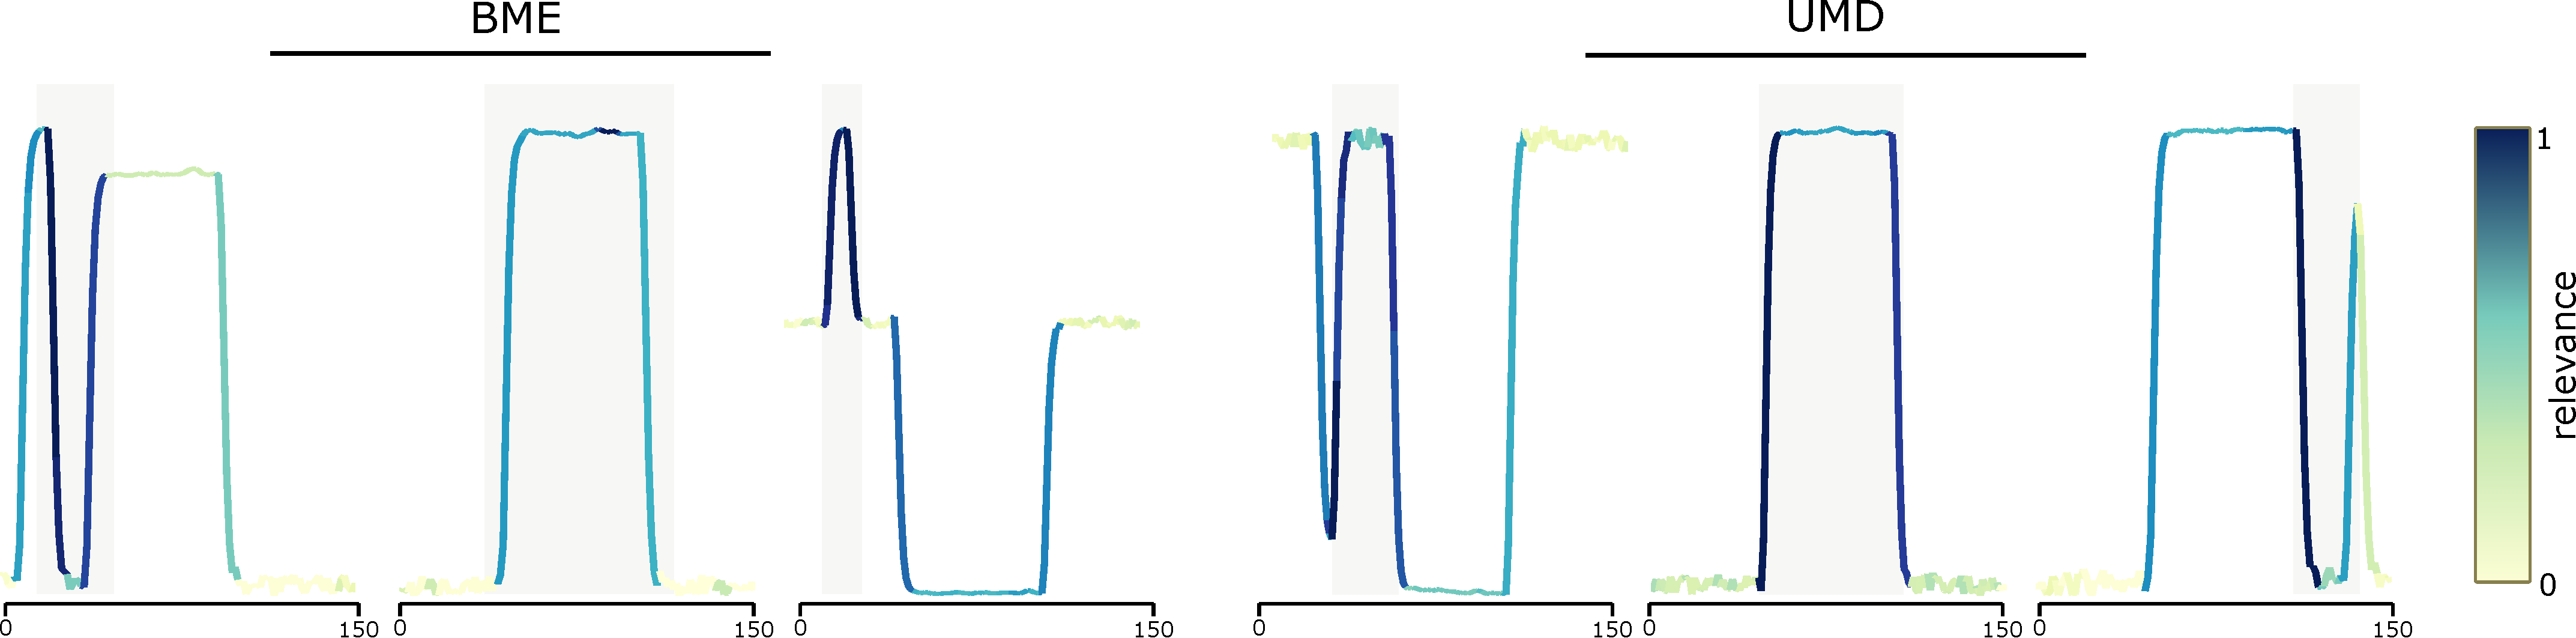
\includegraphics[width=0.95\linewidth]{interpretable_umd_bme.pdf}
    \caption{Interpretable results with highlighted shapes for the \textit{UMD} and \textit{BME} datasets. The \textit{UMD} dataset was classified with with an accuracy of 100\%, computed with a $w_s=10$, $thr=0.05$ and a $2-gram$. The \textit{BME} was classified with an accuracy of 100.0\% with a $w_s=10$, $thr=0.05$ and a $2-gram$}
    \label{fig:interpretable1}
\end{figure}

On Figure \ref{fig:interpretable1} are showed two similar datasets. The f1-score of this task was $1$, meaning that it was able to perfectly characterize each shape with the textual representation. For instance, the \textit{BME} dataset has two different sequences of shapes, since the first class has a \texttt{peak followed by a positive plateau}, while the third class has a \texttt{peak followed by a negative plateau}. The second class has simply a \texttt{plateau}. The main difference between all those classes is the peaks and what follows them, which is precisely what is highlighted. The same happens on the \textit{UMD} dataset, in which the most relevant element is the peak and the plateau. As we can see, the transition from the peak to the plateau is highlighted.
%\par
%The keywords extracted are also intuitive. We extracted the top 3 keywords for all samples of time series of each class. For class 1, the following words are the most common: [\texttt{flat}, \texttt{peak}, \texttt{positive plateau}]. For class 2, the most common words are [\texttt{flat}, \texttt{positive plateau}, \textit{high rise}], while for class 3, common words are:[\texttt{fall}, \texttt{peak}, \texttt{high fall}]

\begin{figure}[h]
    \centering
    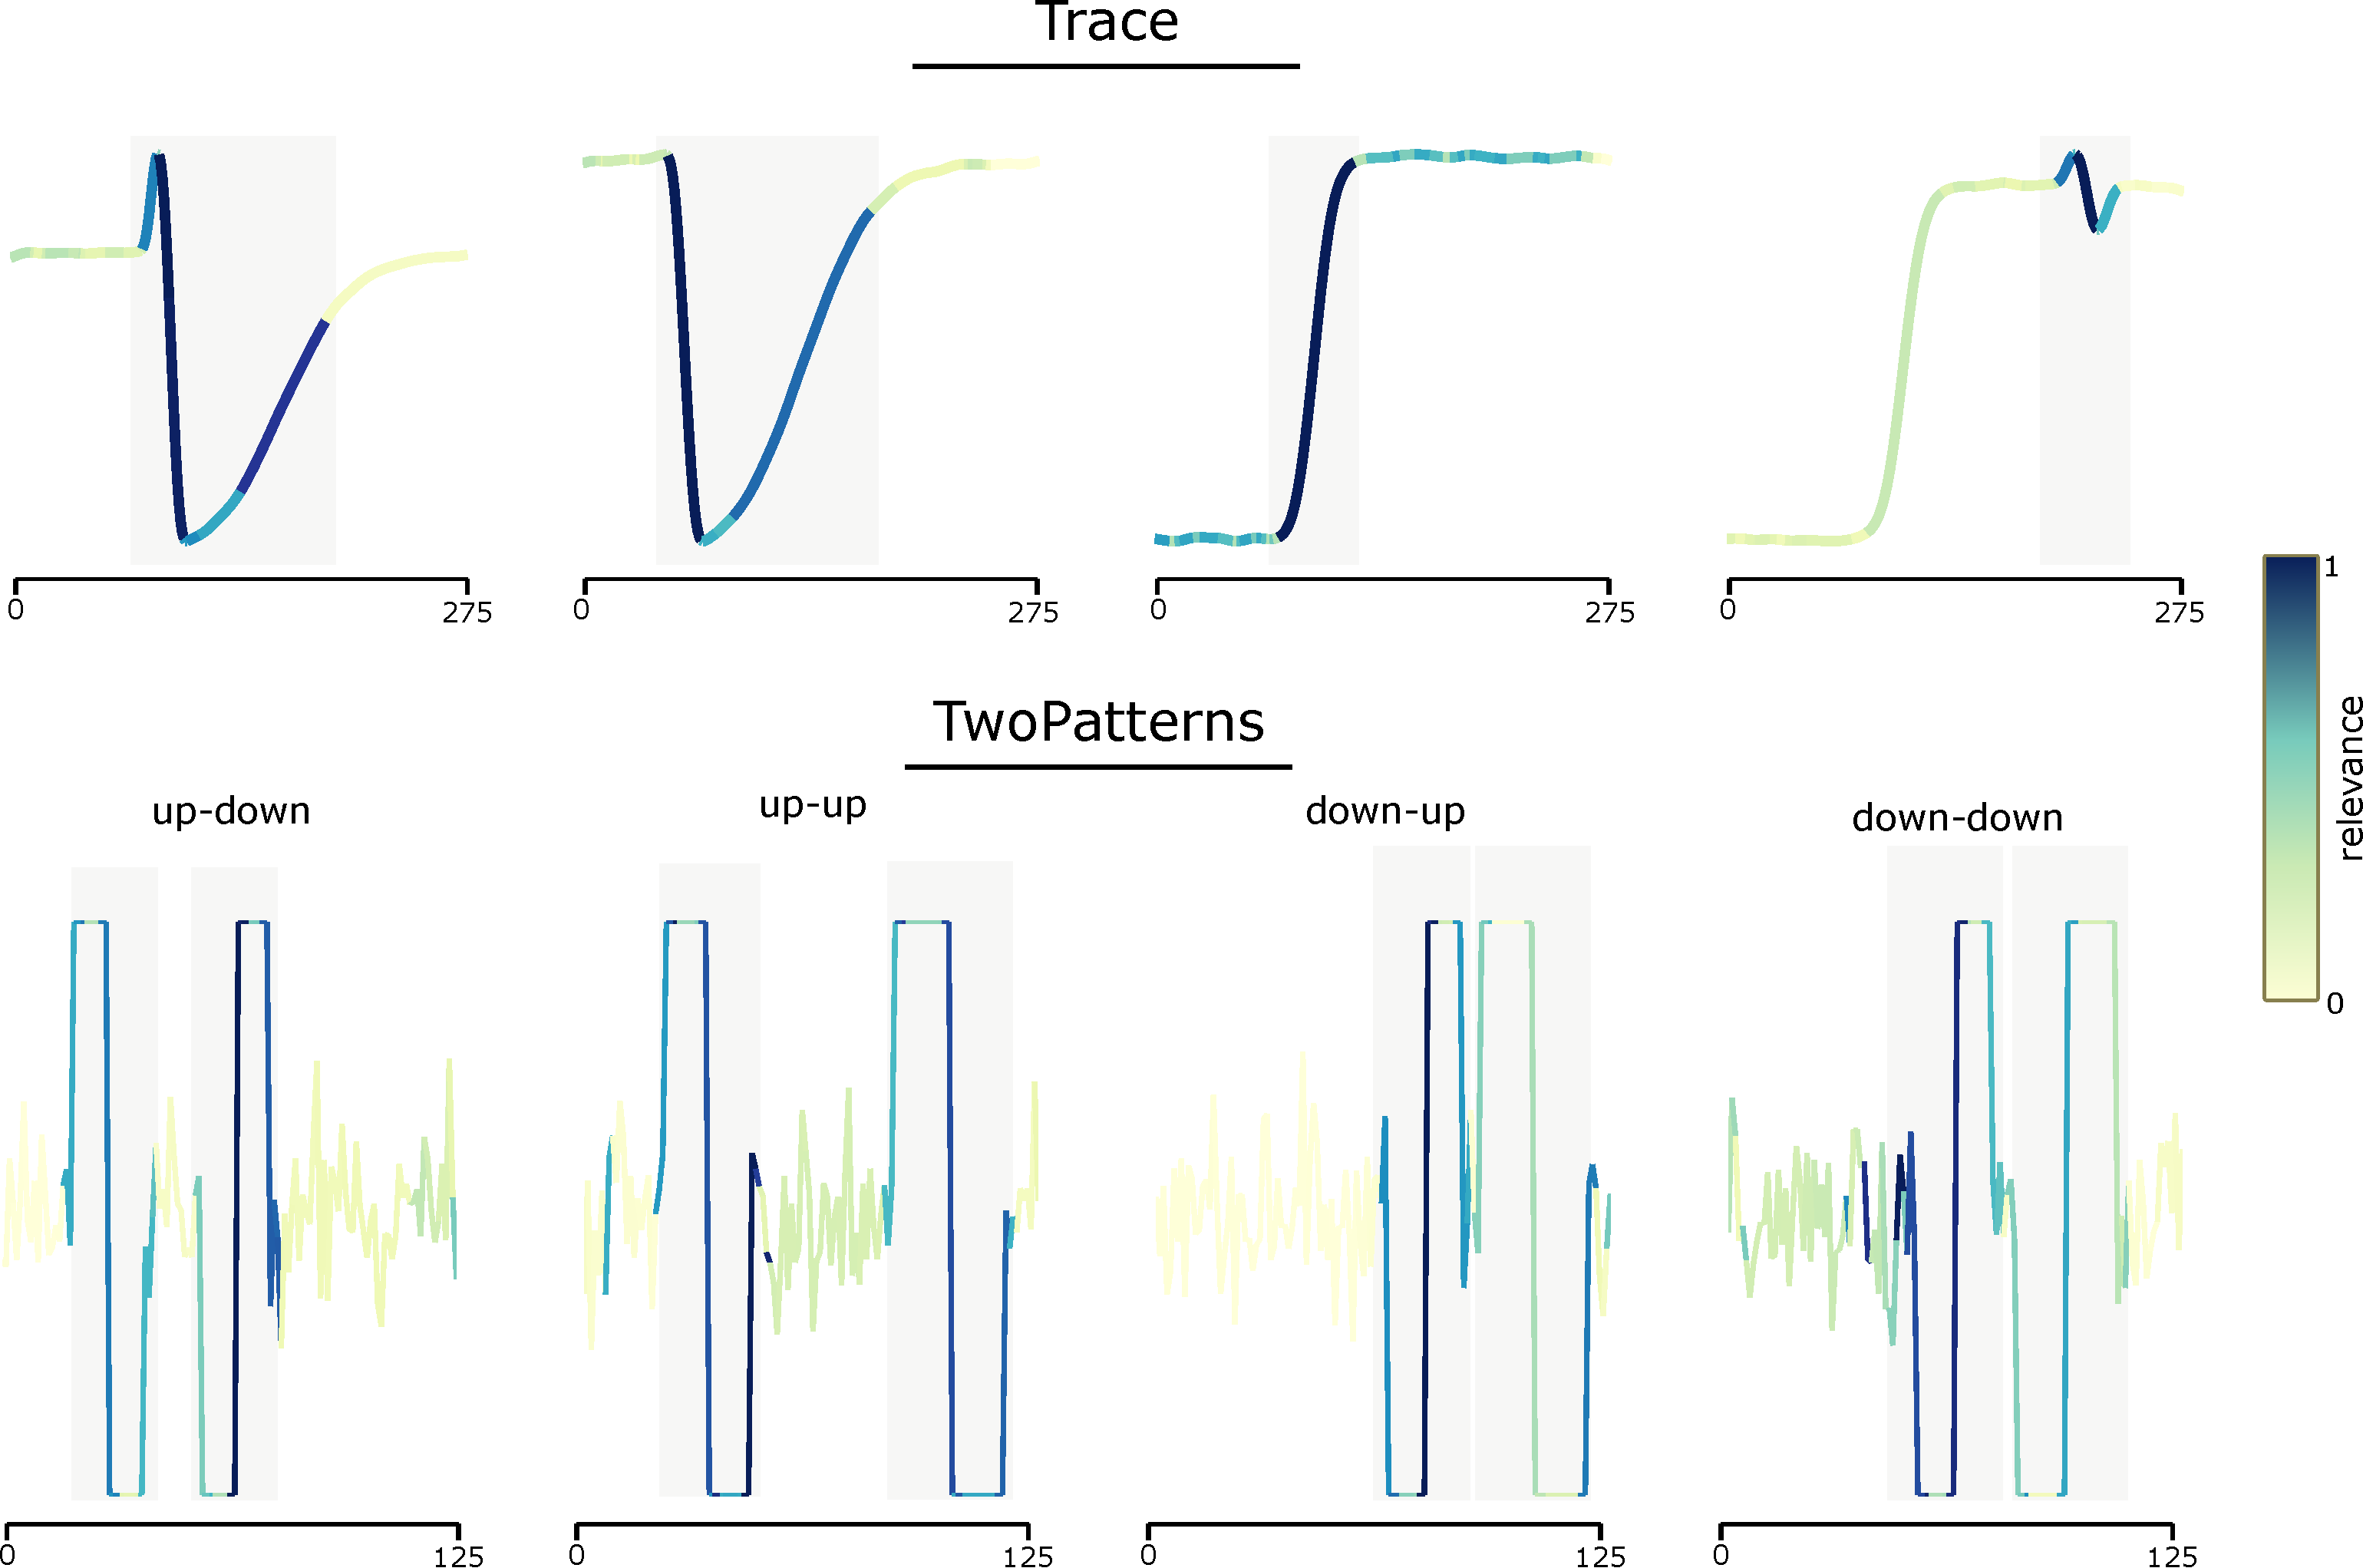
\includegraphics[width=0.95\linewidth]{interpretable_trace_twopatterns.pdf}
    \caption{Interpretable results with highlighted shapes for the \textit{Trace} and \textit{TwoPatterns} datasets. The \textit{Trace} dataset was classified with with an accuracy of 100.0\%, computed with a $w_s=25$, $thr=0.05$ and a $1-gram$. The \textit{TwoPatterns} was classified with an accuracy of 100.0\% with a $w_s=10$, $thr=0.1$ and a $5-gram$}
    \label{fig:interpretable2}
\end{figure}

Another dataset that has intuitive differences between classes is the \textit{Trace} dataset. The \textit{subsequences} of interest are highlighted on each time series of each class. For instance, the first class has the \texttt{peak} and \texttt{valley} highlighted, contrasting with the \texttt{valley} from class 2. Classes 3 and 4 have notoriously different valued elements. While class 3 has the rising phase as the relevant shape, class 4 has a \texttt{small peak followed by a valley} on top highlighted.
\par
The \textit{TwoPatterns} dataset is also intuitive to understand and fits the problem for this experiment. Each class has mostly noise, filled with step functions that have different sequences. Class 1 starts by having an \texttt{up} step function and then a \texttt{down} step function. The same logic is applied to the other classes. The proposed method highlights these step functions as being the relevant segments of the signal.

\begin{figure}[h]
    \centering
    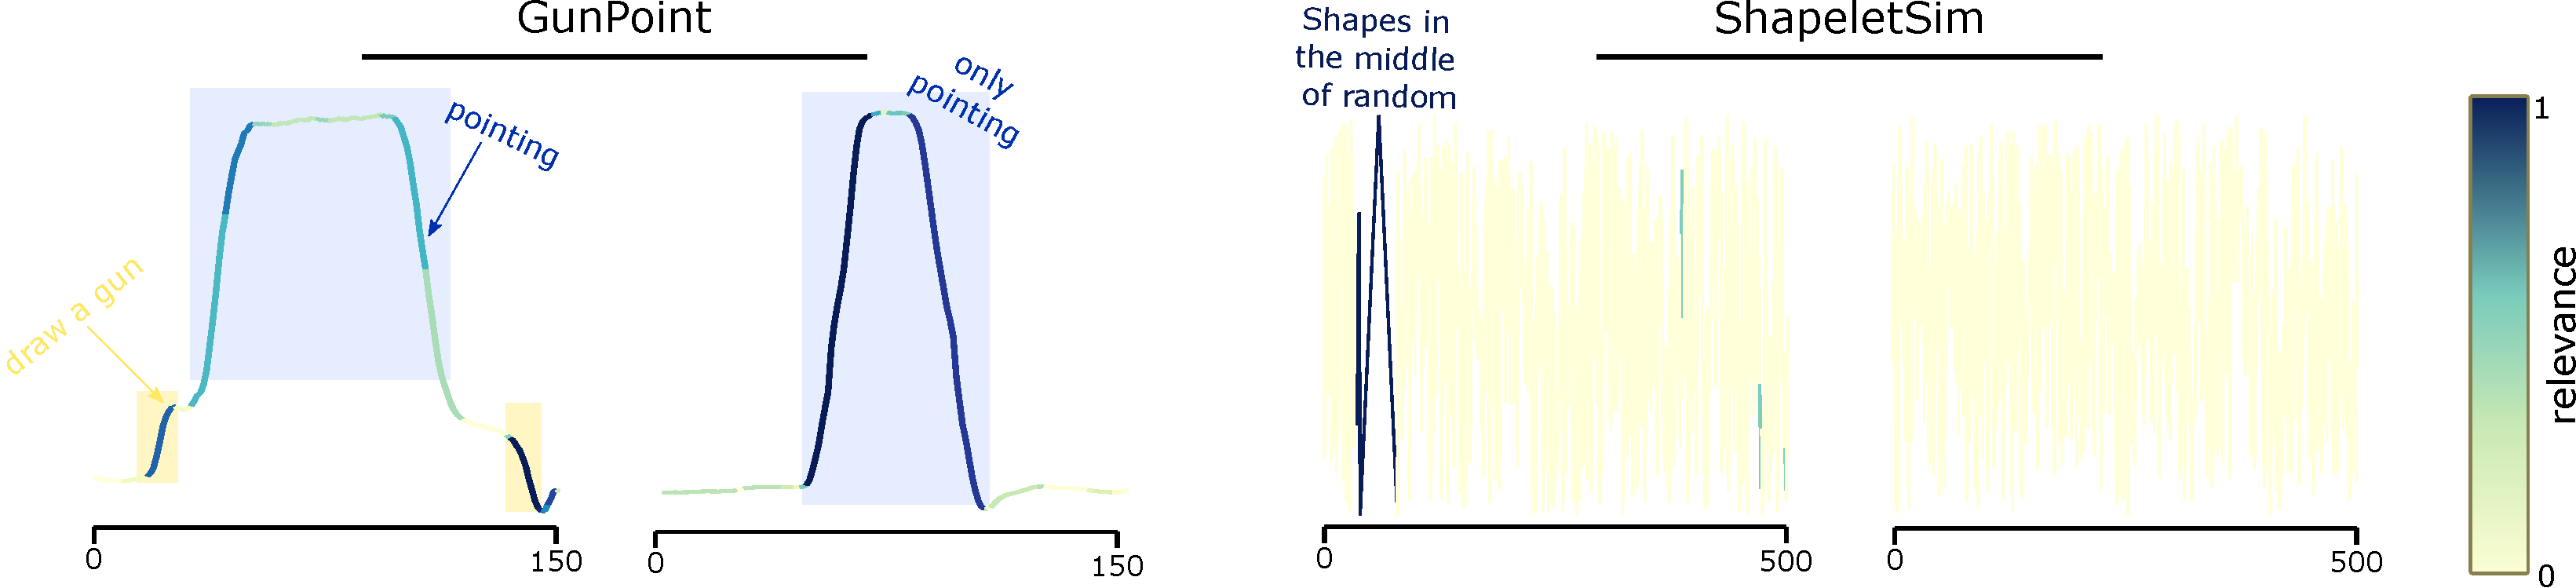
\includegraphics[width=0.95\linewidth]{interpretable_gunpoint_shapeletsim.pdf}
    \caption{Interpretable results with highlighted shapes for the \textit{Gunpoint} and \textit{ShapeletSim} datasets. The GunPoint dataset was classified with with an accuracy of 96.0\%, computed with a $w_s=10$, $thr=0.05$ and a $2-gram$. The \textit{ShapeletSim} was classified with an accuracy of 99.0\% with a $w_s=1$, $thr=0.05$ and a $1-gram$}
    \label{fig:interpretable3}
\end{figure}

Finally, two other examples are also presented. One of the \textit{GunPoint} datasets and another from the \textit{ShapeletSim} dataset. The \textit{GunPoint} has 2 classes: (1) the subject draws a plastic gun and points it; (2) the subject simply points with his/her hand. The major difference between the two classes is the drawing process, highlighted by the method as the \texttt{small rise} and \texttt{small fall}.
\par
Regarding the \textit{ShapeletSim} dataset, the data has also two classes. In one, simple shapes, such as triangular, square, or sawtooth waves were added to a random signal. The method can highlight the representative shape of the signal. 

%Some of the most relevant keywords to distinguish it from the other class are: \textit{low Peak}, \textit{high rise} and \textit{high fall}. 

\subsection{Discussion}
\label{sec:discussion_hearts}

In this section, we wanted to answer two main research questions: (1) can we solve time series classification tasks based on their textual representation following traditional \textit{NLP} methods, and (2) could we use the words that describe the time series to hint about differences between classes of time series. For this purpose, we applied the proposed method on the \textit{UCR} classification benchmark and highlighted several relevant use-cases and the overall results achieved.
\par
The results provide evidence that it is possible to compare time series based on a textual representation and use traditional text-mining strategies for classification purposes. Not only is it possible to compare the vectors of time series documents with the cosine distance (as we have seen on Figure \ref{fig:distribution_dendogram}, but \gls{bow} or \gls{tfidf} models can be used with a linear \gls{svm} to solve classification tasks.
\par
Additionally, the fact that words are weighted based on their relevance to distinguish each time series document from all the others, it is possible to highlight the \textit{subsequences} of the time series corresponding to these words and understand which parts of the signal are more relevant, being a step forward into interpretability of time series. The limited examples were still simple and intuitive and the process turns harder to understand in more complex data. In these cases, it is hard to truly find meaningful differences and explain why these classes are different, especially with words. This limits the further interpretability potential of this method because the differences might not be perceptible by the naked eye. On one end, the performance can be improved using a richer and correct set of textual descriptors. We mean richer because the differentiation is as good as the description performed, and we mean correct because the translation process from the numerical domain to the text domain is not error-proof, which means that a mistranslation may occur and make the results worse. This fact can also contribute to the lack in ability to generalize the model from the cross-validation to the validation steps, with an evident decrease in performance.

Another relevant point is the fact that words used might not be capable of expressing the differences between classes. Many cases with high accuracies can be highlighted, but their interpretability falls short. For instance, for the dataset \textit{ECGFiveDays}, a binary classification problem. The method has 0.96 of accuracy, but does not show expressively the difference between classes.
\par
The textual representation is valuable in the sense that text mining domain knowledge can be used on time series. Nevertheless, we can profit from this knowledge as much as the translation of the time series into text is rich, valuable, and domain-specific. With the current set of \gls{ssts} queries we can make a limited description that works well in simple signals described mostly by their derivative dynamics. The keywords extracted for these time series still have limited readability being even harder for more complex examples. However, if more expressive queries are used to make a more robust translation, the keywords extracted can be more valuable and relatable to the time series we are looking at. Therefore, a more diverse set of queries should be used to make possible the extraction of more relevant keywords. At some point, a reduction and selection of the most relevant keywords should be made.

\section{Pattern Search with QuoTS}

In this Section, we demonstrate the potential utility of \gls{quots} to search for relevant subsequences in real datasets. Table \ref{tab:operators} from the previous Chapter highlights the keywords and operators if needed to follow these examples. This method, in contrast with \gls{ssts}, uses features and not a symbolic representation of the time series.
\par
In order to show evidence that \gls{quots} is useful in a multitude of scenarios, we present several examples of its application to find relevant patterns on real domain time series. The section will start by presenting how well it matches hand gestures; then show its applicability in searching for relevant patterns in several problems and use-cases; and finally, we present the ability to include additional words based on existing patterns, with the example of \textit{puppeteering} a toy car model.

\subsection{\textit{QuoTS} Matches Gestures}

We start by demonstrating the ability of \gls{quots} to sort how well individual shapes match a written query. For this, we used the \textit{UWaveGestureLibrary} dataset from the \textit{UCRArchive} as a proxy \cite{uWave}, which similar to telemetry data, relies on inertial time series. We use this proxy data simply because it is much larger than any publicly available labeled transportation data. However, we note that gestural interaction with the automobile interfaces is an area of active research \cite{autoui1, autoui2}. With this example, we show that the system can recognize different gestures with or without intuitive queries, hence, if humans were able to learn and master this tool, this recognition problem would be largely solved.

\begin{figure}
\centering
\includegraphics[width=\linewidth]{quots_wavegestures.pdf}
\caption{\textit{UWaveGestureLibrary} subsequence matches with \gls{quots}. Column-wise are showed the gesture class, the corresponding mean wave for all subsequences, the query used to match the subsequence class and the corresponding match score for all subsequences, highlighting with the color of the specific class.}
\label{fig:quots_uwave}
\end{figure}

We not only demonstrate that the system can significantly distinguish gesture patterns, but it does so with very simple and intuitive queries. The ability of the written queries to match the correct class is presented both visually (Figure \ref{fig:quots_uwave} and quantitatively (Table \ref{tab:quots_exp1}). In Figure 5, the set of eight gestures is described row-wise, having a corresponding mean shape (\textbf{MeanWave}) and a query (\textbf{Query}) that should filter it. The visual intuition is demonstrated with the barplot (\textbf{MatchScore}), which for the sake of readability, highlights the normalized match score ([0-1]) of subsequences belonging to the row-wise specific gesture. The other classes are shown in gray. For each gesture, we show the shape of all the available axis (X, Y, and Z). We attempt to create queries using only a single axis (X-axis) but used other dimensions when needed.
\par
To quantify these results, we looked at the top-10 and top-100 matches for each class and counted how many gestures of the selected class were correctly sorted (TP/10 and TP/100). The results are presented in Table \ref{tab:quots_exp1}. These show that the top 10 matches always correspond to the correct class. The reader might think that the first 10 matches might be too easy considering a problem that has around 400 gesture samples per class, but note that having more gesture samples also means more opportunities to make mistakes. Moreover, considering the analogy of searching for a webpage with the \textit{Google} search engine, a user will probably be interested in examining at least the top 10 results. Nevertheless, the reader will appreciate that even if we consider the top 100 matches, \gls{quots} still achieved impressive results.

\begin{table}
\centering
\begin{tabular}{ccccccccc}
\toprule[1.5pt]
& G1 & G2 & G3 & G4 & G5 & G6 & G7 & G8\\
\midrule
TP/10 & 10 & 10 & 10 & 10 & 10 & 10 & 10 & 10\\
TP/100 & 96 & 100 & 94 & 95 & 74 & 100 & 100 & 99\\
\bottomrule[1.5pt]
\end{tabular}
\caption{Results for the top 10 and top 100 sorted gestures classes  (G) when using the queries from Figure \ref{fig:quots_uwave}.}
\label{tab:quots_exp1}
\end{table}

Although we simply wanted to demonstrate that with a set of meaningful words we can correctly sort each of the classes of this dataset, we also want to highlight that the nature of the classes can be very well expressed by the queries. This is especially evident when we look at the query for gestures that are inverse to each other, such as gestures 7 and 8. Gesture 7 is well matched by the query \texttt{[valley peak]}, implicitly, the transposed gesture should have the exact opposite query, which it indeed does (\texttt{[peak valley]}). This also occurs for the two other sets of gestures that occur in natural pair; gestures 3 (\texttt{[bottom up up top] simple}) - 4 (\texttt{[top down down bottom] simple}) and gestures  5 (\texttt{[top down down bottom]}) - 6 (\texttt{[bottom up up top]}).
We also demonstrate that for the handful of cases where this did not work, there was a semantic explanation for it. (e.g. Classes 5 and 6 have not a specific pattern and seem to be especially random in their X-axis, or classes 1 and 2 are very similar, and because of that, are mislabeled). But, as our tool can perform queries in multidimensional data, we can still discriminate these by using the Y-axis in conjunction with X-axis to sort them correctly. 
Note that discriminating among these eight classes is not a trivial problem. Of the more than 1,000 papers to have worked with this dataset, the current best accuracy was obtained by \textit{COTE} algorithm which achieved 76.56\% using a single axis. In addition, this dataset was acquired from eight different subjects, which indicates that our system can account for the intra-subject and inter-subject variability in motion for this dataset \cite{uWave}.

\subsection{\textit{QuoTS} in Selected Use Cases}

In this section, we present several examples of where \gls{quots} can be used in continuous real data. We start with an \gls{ecg} signal that has motion artifacts.

\subsubsection{Pattern search on the \gls{ecg}}

\begin{figure}
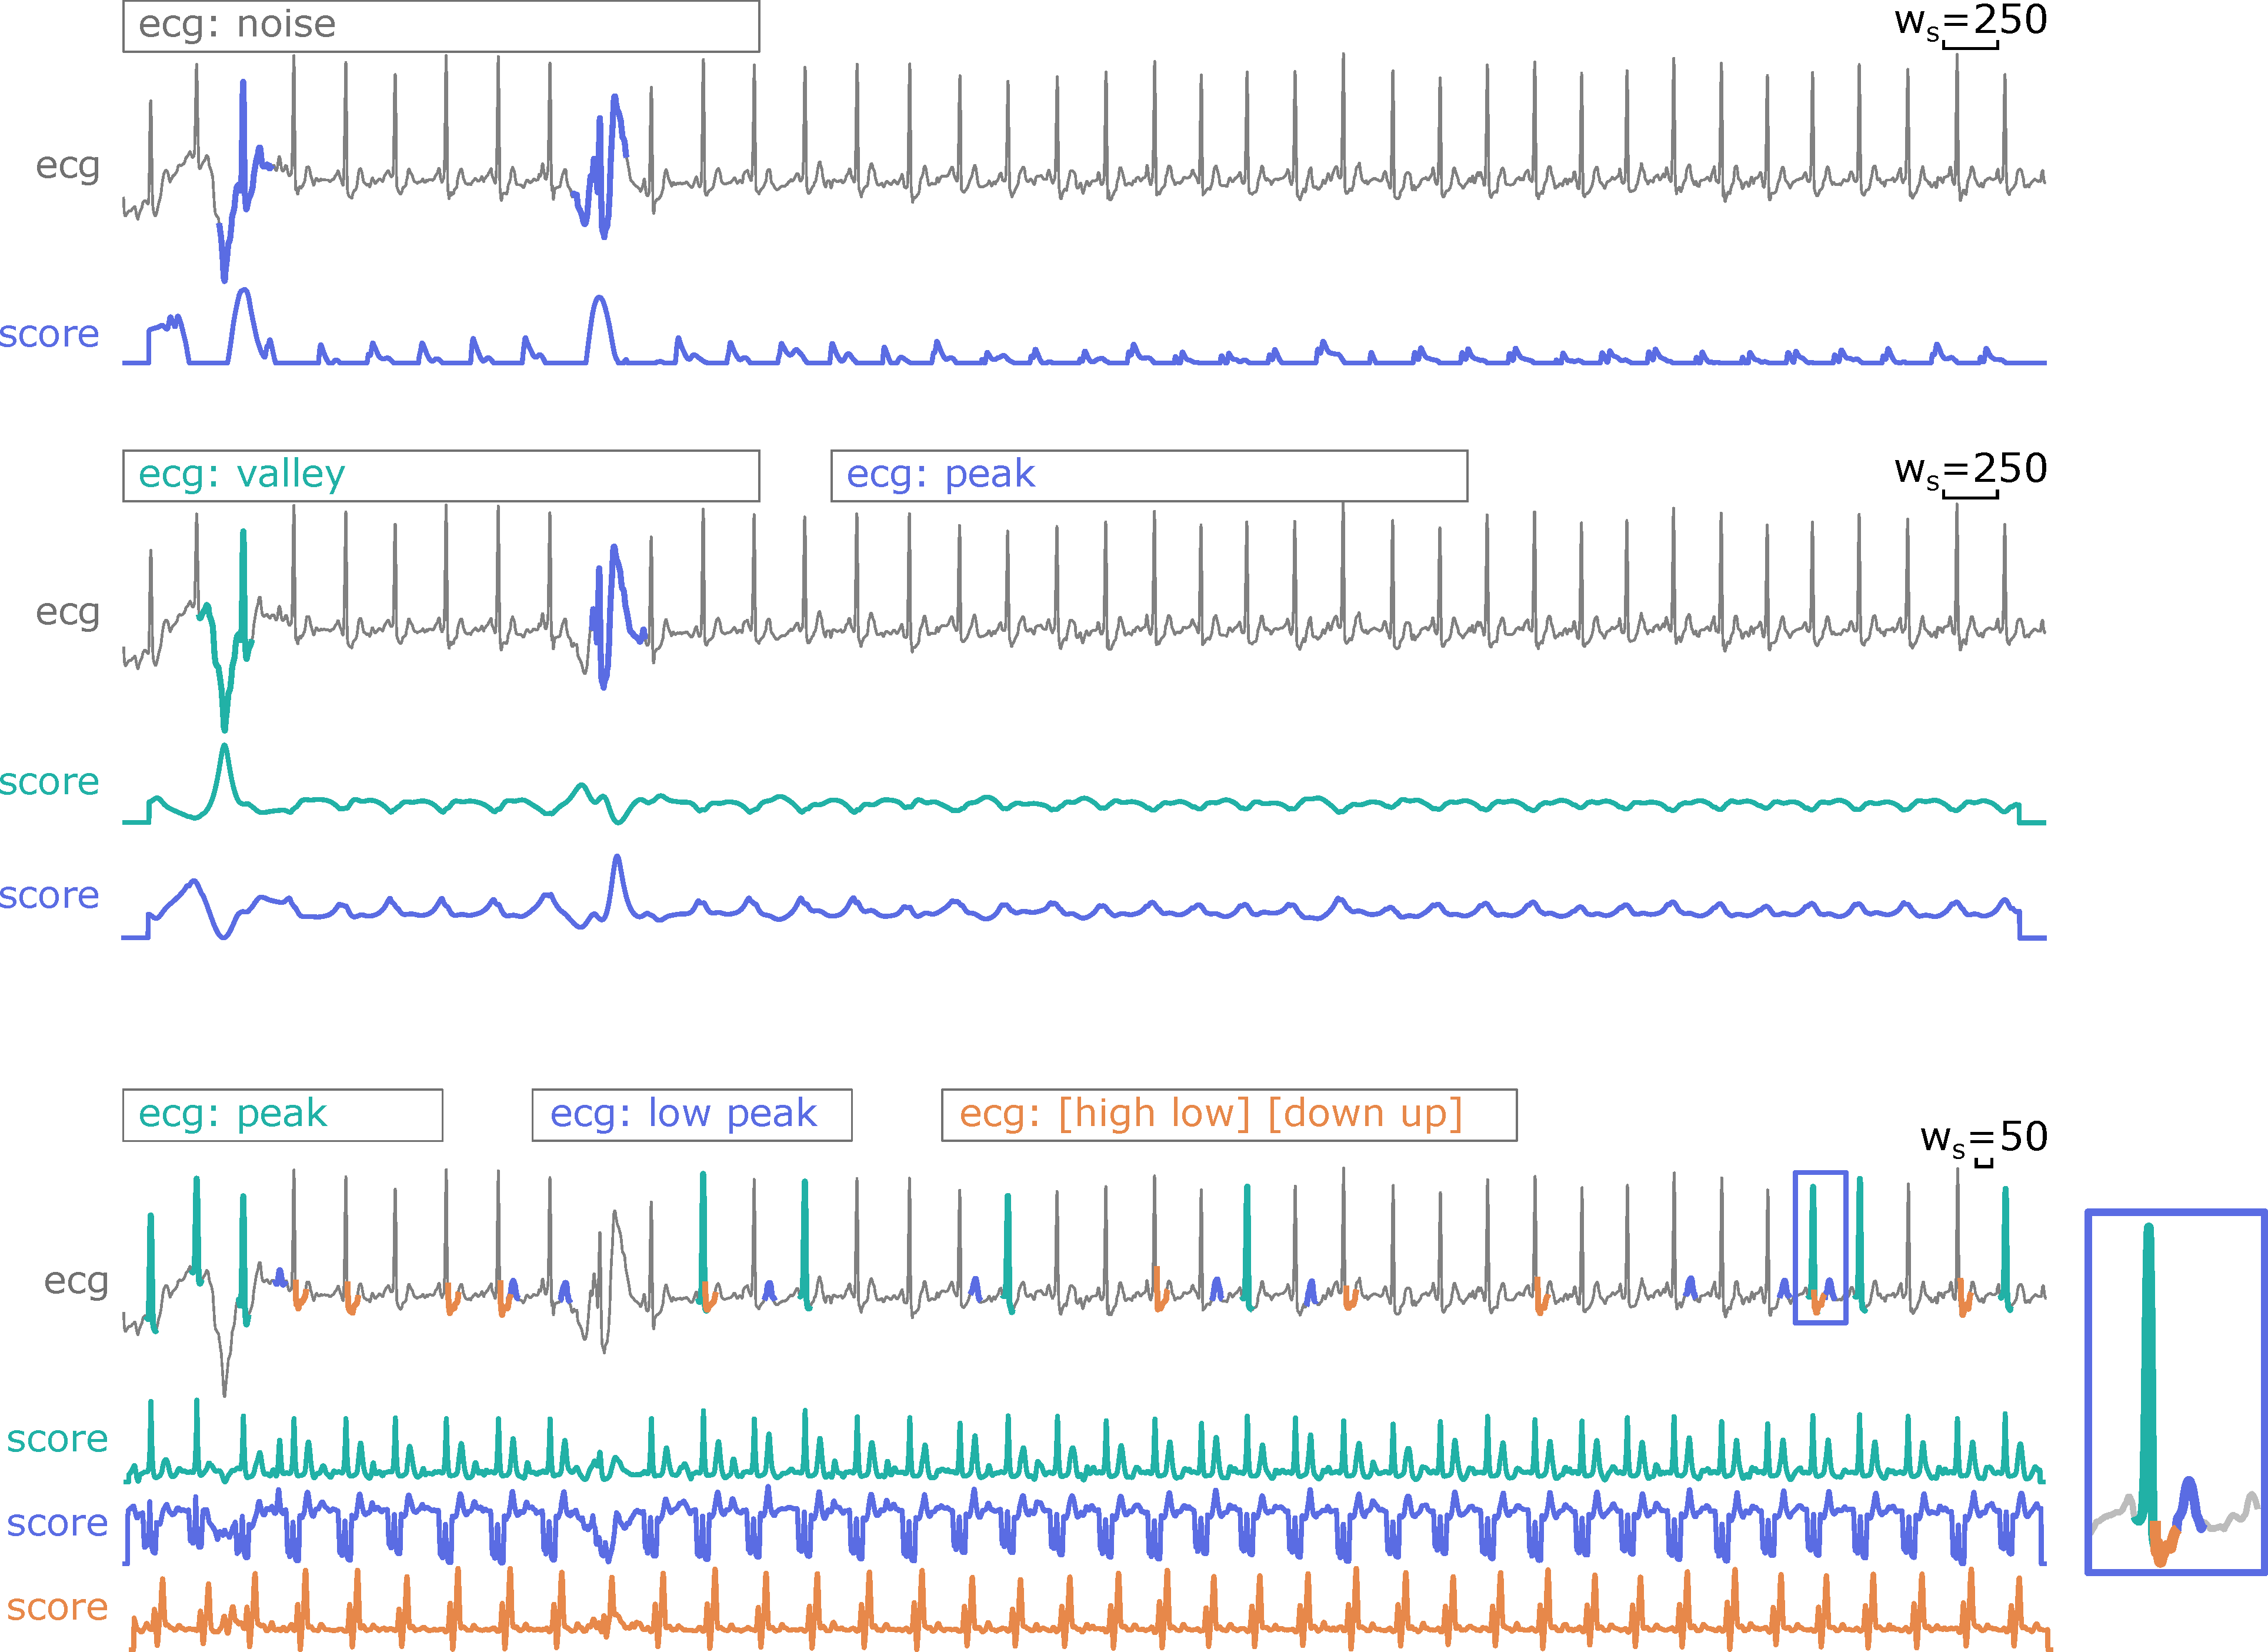
\includegraphics[width=\linewidth]{Quots_ecg.pdf}
\caption{\gls{ecg} use case to identify noisy sections, as well as specific segments of the \gls{ecg} pattern. The queries are written in text boxes. On the side, an example of a match is shown as a larger pattern.}
\label{fig:ecg_use_case1}
\end{figure}

As a start, we were searching for the motion artifact segment that appears in two areas of the signal. This artifact can be detected in two ways, as we are showing in Figure \ref{fig:ecg_use_case1}. The first would be to use the keyword \texttt{noise}, which searches for parts of the signal that have a higher difference from a moving average of the signal. In this case, the higher difference occurs when the motion artifacts appear. We could also search for each of these motion artifact sequences simply by pure visual intuition of their shape. For instance, the first motion artifact looks like a \texttt{valley}, while the second looks like a \texttt{peak}, which ends up matching the desired segments. This process was made by looking for subsequences with 250 samples.
\par
On the \gls{ecg} signal, we can also find other segments of interest, namely from the \textit{PQRS} complex. In this case, we searched for the \textit{R} \texttt{peak}, the \textit{S} \texttt{valley} and the \textit{T} \texttt{peak}. The first subsequence was simply matched by searching for the keyword \texttt{peak}, with a window size of 50 samples, which contrasts with the 250 samples from the previous example. The keyword matched well the highest peak, but other peaks were present with lower amplitudes, such as the \textit{T} \texttt{peak}. This one was matched with the query \texttt{low peak}. In between these two subsequences, there is the \textit{S} \texttt{valley}. In this case, we show the usage of the special \texttt{followed by} operator. The query \texttt{[high low] [down up]} indicates that the first half of the searched subsequence should have a \textit{high change in amplitude going down} and ends with a \textit{low change in amplitude going up}. This is exactly what is matched, as highlighted and indicated by the corresponding \textit{score} function. To be clear, the colored highlighted segments represent the 10-most relevant matches for the written query. The \textit{scoring} functions show that the other matches would be found as well.
\par
The \gls{ecg} signal is a perfect example of how a text-based search can help find relevant occurrences, as we showed previously. However, there are occurrence of higher interest, such as patterns linked to specific medical conditions that are represented by variations in the original shape of the \gls{ecg} signal. Figure (\ref{fig:ecg_use_case2}) shows several examples of the detection of three different types of arrhythmia from the \textit{St Petersburg INCART 12-lead Arrhythmia Database} (Physionet) \cite{PhysioNet}.

\begin{figure}
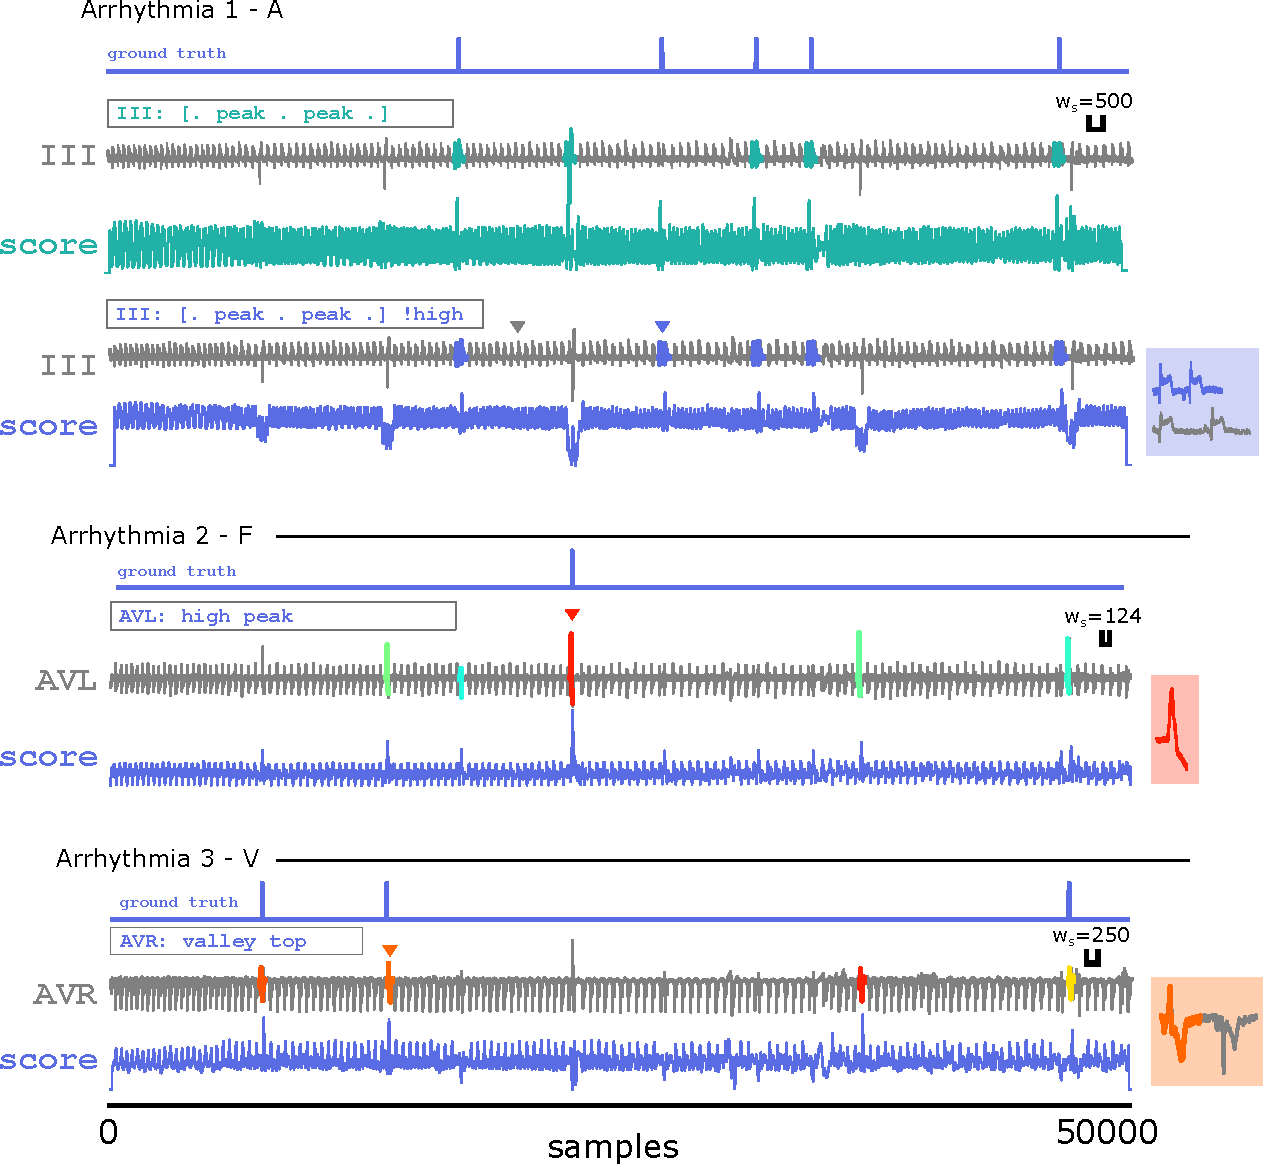
\includegraphics[width=\linewidth]{Quots_ecg2.pdf}
\caption{Examples of the detection of three specific cases of arrhythmia. The ground truth is selected from the annotations of specialists in the area. The queries are presented in text boxes and the found patterns are highlighted. On the side, an example of a match in a larger size is shown.}
\label{fig:ecg_use_case2}
\end{figure}

The ground truth follows the annotations present on the original files. Three types of annotations were found, associated with different types of arrhythmia events (A - 
\includegraphics[height=2.5ex, valign=m]{arrhytmia_A.pdf}, F - 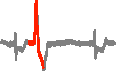
\includegraphics[height=2.5ex, valign=m]{arrhytmia_F.pdf} and V - 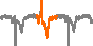
\includegraphics[height=2.5ex, valign=m]{arrhytmia_V.pdf}). Using \gls{quots}, we can search for these occurrences in the presented segment. The first event is characterized by having a normal beat irregularly before it was supposed to. It is then possible to find two \gls{ecg} beats in a shorter window. This means that if we search for two main peaks inside a short window, separated by anything (\texttt{.}) \texttt{III: [. peak . peak .]} (in this case 500 samples on the lead III), it should be possible to find where these events occur. We displayed the 5-top subsequences that match the query and the corresponding scoring function. Four out of the five events are highlighted, but the scoring function indicates that the "missing" subsequence has a high match value as well. The wrongly identified event fits the description as well, being a different type of arrhythmia, but with a different shape (type F). This shape is normally a high change in amplitude, therefore if we state that we reject any high amplitude change subsequence, we should be able to match the five desired subsequences. Adding \texttt{!high} to the previous query (\texttt{III: [. peak . peak .] !high}) leads to correctly matching all the desired subsequences. To be clear, we chose lead III without any specific purpose, being possible to use the other leads for the same purpose. What matters is that the desired subsequence has a particular characteristic that differentiates it from the rest.
\par
The second example corresponds to the arrhythmia of type F, characterized by a high change in the amplitude of the \gls{ecg} with an irregular beat. In this case, we can match this event with the simple query \texttt{AVL: [high peak]}. Other events are matched but have a much lower amplitude. The other events matched are from the type V, which does not present a long flat section after the irregular beat. In this case, the lead AVR shows a very specific difference from the other two types of arrhythmia, which is the fact that the beat occurs on top, deviating from the middle of the signal. The shape continues to be a \texttt{valley} but on \texttt{top} (\texttt{AVR: valley top}). It is relevant to point out that the original annotations (ground truth) do not include one of the highlighted subsequences. Although not confirmed with a specialist, the shape of the event in all \gls{ecg} leads are the same for this type of arrhythmia, so we suspect that there was a missing label that the query was able to indicate.

\subsubsection{Pattern search on multimodal signals}

In addition to searching for specific shapes on signals, \gls{quots} can be very useful for exploratory purposes in multivariate datasets. For instance, consider the following examples on a dataset acquired with the purpose to identify workload on drivers \cite{hcilab}. In this experiment, drivers physiological signals, such as \gls{ecg} and \gls{scr}, were monitored. Exploring this dataset with \gls{quots} led to discovering several interesting occurrences, as shown in Figure \ref{fig:quots_car_physio}. In this Figure are signaled specific events with road signs. We matched these signs' positions by finding their \textit{latitude} and \textit{longitude} on the map and matching them with the instant in time these coordinates occur on the dataset. In addition to this information, we recall the common terms used for auto telemetry, namely: Surge - breaking (peak) and accelerating (valley); and Sway - turning right (peak) or left (valley).

\begin{figure}[h]
\centering
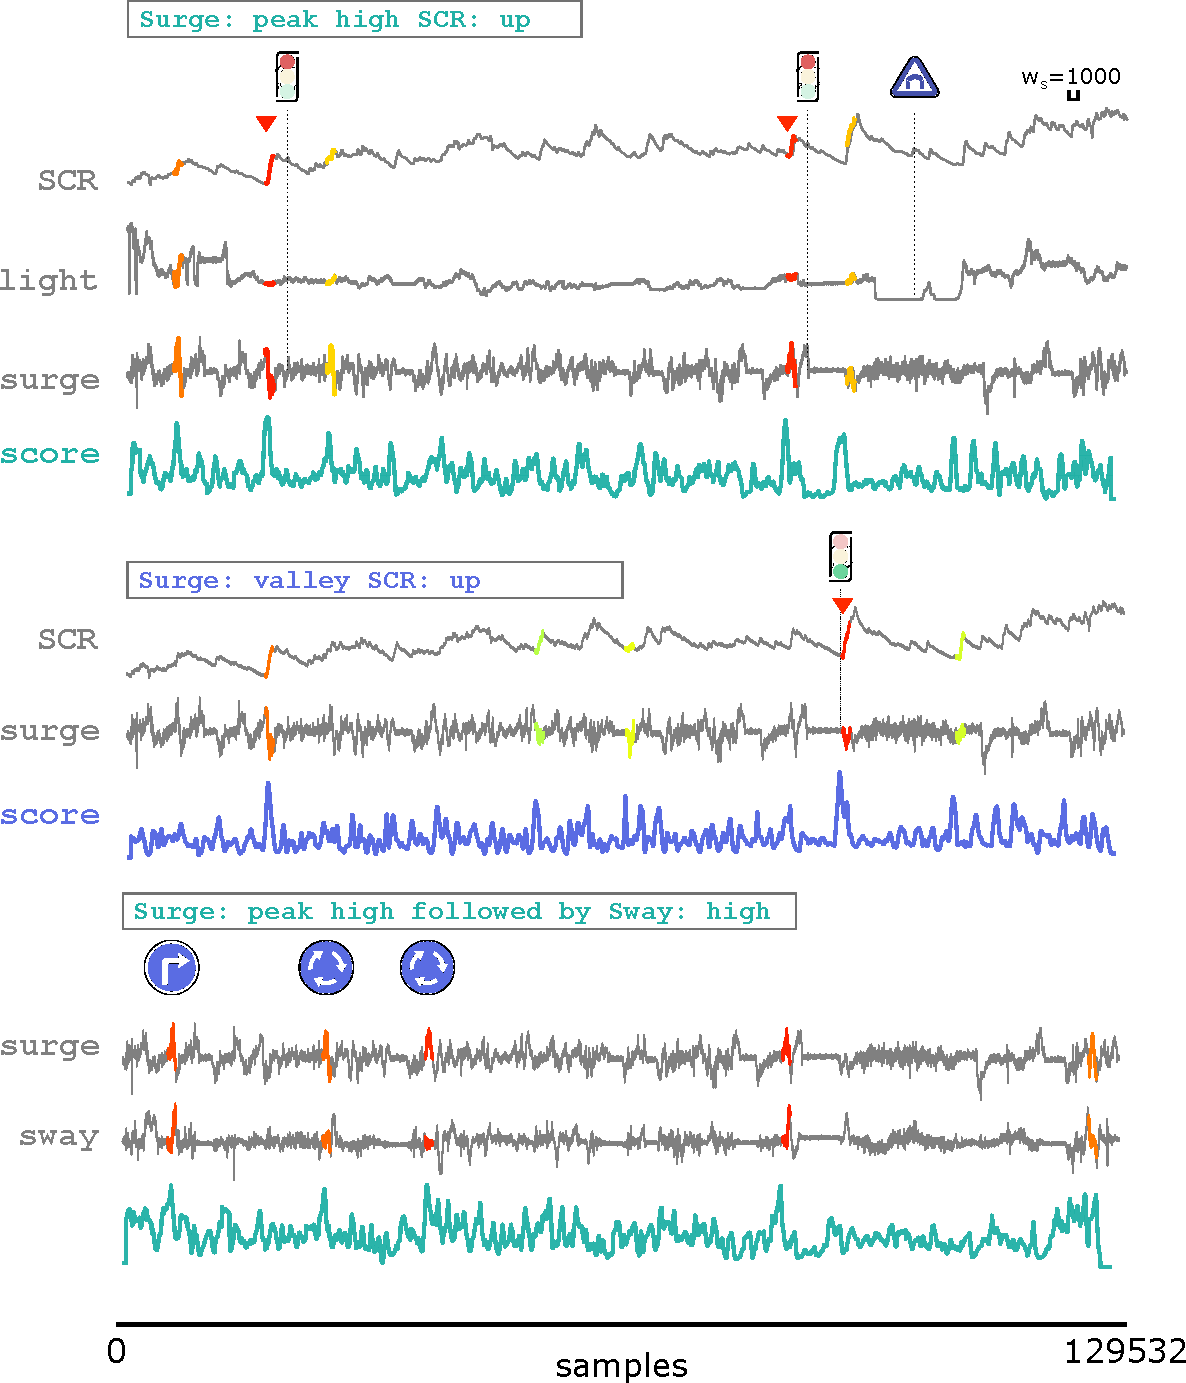
\includegraphics[width=0.85\linewidth]{quots_car_bio.pdf}
\caption{Example of multivariate patterns on a dataset from auto telemetry with physiological signals of the driver. The queries are written in text boxes. Several matches are highlighted based on the queries written. These events are associated with specific occurrences during the driving session, symbolized by traffic signs. These events were matched by searching the coordinates on the map. \cite{hcilab}}
\label{fig:quots_car_physio}
\end{figure}

The first found events were identified by searching for moments where the driver was pulling the breaks and at a similar moment in time, the driver was having an increasing value of skin conductance (indicative of higher sweat and possibly momentary stress). The query can be written as \texttt{Surge: peak high SCR: up}. We found that the presence of such events is very high on two occasions, in both cases, right before a traffic light. The second traffic light was turned red because the car stopped. This led to searching for a moment where the driver started accelerating and the skin conductance was increasing (\texttt{Surge: valley SCR: up}), which points to two main locations on the signal. The second is exactly when the car started driving after stopping at the traffic light, suggesting to be a relevant reaction from the driver. We did not have access to the videos, and can only guess what happened during the driving experience, but we can conclude that these identified moments are relevant to be observed afterward on the video, highlighting that \gls{quots} can be used to explore the signals very quickly, identify moments of interest (especially correlating multivariate variables) and search them on the video to validate what happened. 
\par
In addition to these events, we searched for moments where the driver had to break and then turned. There is a time dependency between these two occurrences and can use the \texttt{followed by} operator for this purpose. Therefore, we searched for \texttt{Surge: peak high followed by Sway: high}. The results pointed out several locations on the signal, three of them associated with turning right at a crossing and two roundabouts.

\subsection{Matching \textit{Known} Shapes with Words}

We believe that \gls{quots} can be developed to be intuitive enough to allow most novice users to create simple effective queries for most information retrieval tasks.  However, in some cases, the user’s ability to formulate queries may be a limitation. In this section, we show that it is possible to perform a \textit{mimicry} of the process being searched and add the query designed with the mimicry process as a \textit{word feature vector} inside our vocabulary. We show a few examples of possible applications, starting with "puppeteering" a model car in performing a 3-point-turn. First, we will show the signal where we searched this event and how we used \gls{quots} to find it with a text query.

\begin{figure}
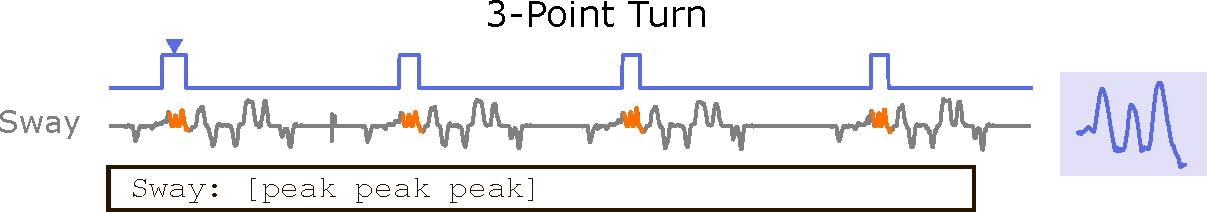
\includegraphics[width=\linewidth]{quots_3pointturn2.pdf}
\caption{Example of searching for a 3 point turn event with \gls{quots}.}
\label{fig:quots_3pointturn}
\end{figure}

Figure \ref{fig:quots_3pointturn} shows the search for a 3-point turn on a signal acquired with a smartphone inside a car while performing several driving exercises in a parking lot. Details of the experiment can be found at the Github repository \footnote{\url{https://github.com/Anonymous14151/QuoTS}}. The query used to match this event is very intuitive, being \texttt{[peak peak peak]}, which is exactly what this pattern is (
\includegraphics[height=2.5ex, valign=m]{3pointturn.pdf}). 
\par
Having found the desired pattern with text, we thought that it would also be possible to find it using a specific pattern and give it a name to use on \gls{quots}. In this case, the pattern was acquired with a toy model car, on which a smartphone was attached (as indicated in Figure \ref{fig:puppeteering}) and acquired inertial data while mimicking a 3-point turn event on a table. The resulting shape is illustrated in \textit{puppet data}. We believe this can be used in two ways: for the user to gain intuition as to how a motion/\textit{manoeuver} is illustrated on motion data or how the inertial data from the motion/\textit{manoeuver} can be used as a template on \gls{quots}: \\
•	\textbf{Shape Intuition:} A user might not know what the shape of a 3-point turn looks like. By using a model car, he/she can mimic the motion and gain intuition over what the query should be (in this case, \texttt{[peak peak peak]}). \\
•	\textbf{MASS template:} As mentioned above, we have a special shape word, which corresponds to a shape template given by the user, to which a word can be assigned. We then can use the word in our language to match desired patterns with the MASS distance profile as a word feature vector.  

\begin{figure}[h]
    \centering
    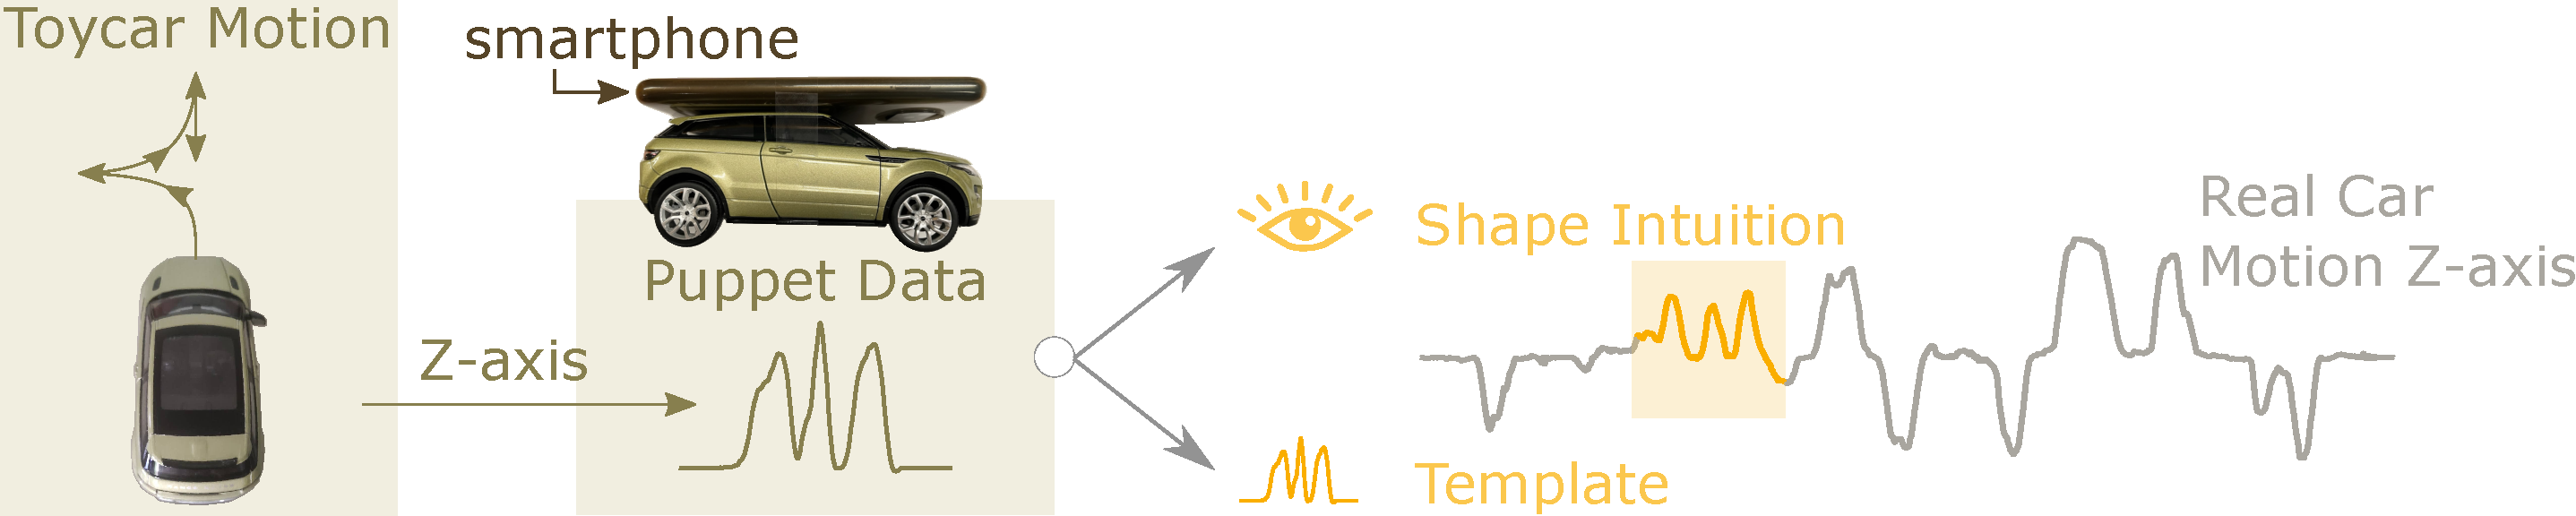
\includegraphics[width=0.95\linewidth]{toycar_puppet_example.pdf}
    \caption{Creating query prompt data by puppeteering a car model. The puppet data for a 3-point turn (smoothed with 10 samples moving average) is presented on the left, while the real data from a real car is presented on the right. }
    \label{fig:puppeteering}
\end{figure}

We added the puppet data and the word \texttt{3pointturn} to our vocabulary. Searching for it in the signal matched all the desired shapes. Note that the template has a different amplitude and time scale considering that the motion was made with our hand, but the z-normalization makes the amplitude difference irrelevant, and the time scale was adjusted by resampling the template based on the selected window size for the query search. With this, the template is not only a template, it also becomes part of the language, being used in combination with all the other words available in our vocabulary.



%\subsection{Segmentation 3: Storytelling Data}
%
%As a concluding note, we believe this method support telling the story behind the data. It can help identify moments that are relevant and try to figure out their meaning with minimal context. For instance, taking the example of Figure \ref{fig:autoeuropa_ssm}, a collaborator was performing workstation 1, was interrupted for a long period, restarted to perform workstation 1, and then shifted to workstation 2. This sequence of events is possible to be seen on the \gls{ssm} of the signals monitored.
%
%
%
%
%
%%For instance, before showing an example of the occupational domain, let us show the reader an example of Dataset 4.
%%


%%\begin{figure}
%%    \centering
%%    \includegraphics[width=\linewidth]{Clustering_real_difficult_timeseries.pdf}
%%    \caption{Activity segmentation and clustering based on the \gls{ssm} for an example of Dataset 4. The activities are color coded, as well as the segments identified by the analysis of the \gls{ssm}. These are then clustered based on the similarity profiles (which are also colorcoded on the dendogram).}
%%    \label{fig:example2_har}
%%\end{figure}
%%
%%Figure \ref{fig:example2_har} shows a signal with several activities (as described in Section \ref{subsec:uci}). The transitions are relatively easy to identify. After segmenting these transitions, we can sort them by their corresponding activity class. Besides, all subsequences related to standing (standing, walking, climbing, or falling stairs) are grouped, while static postures such as sitting or lying are closer together.
%
%\subsection{Storytelling Occupational Data}
%\label{subsec:storytel}
%
%1 - Example of the data we acquired in Volkswagen when we arrived and tried to compare two workstations. We were trying to find specific cyclic moments and labeled them by hand. We can use this tool to make this identification (SSM):
%
%1.1 - show the matrix of the data
%
%2 - Describe the pattern using words or a \gls{regex}
%
%
%
%\subsection{Pattern Search in Occupational Data}
%\label{subsec:search}
%
%\section{General Limitations}
%
%In this section we present the general limitations of the presented methods, following the results achieved.
%
%\subsection{Information Retrieval with the SSM}
%
%- size and memory consumption
%
%- feature reduction
%
%- feature specific
%
%- The method to retrieve the diagonals is not good enough
%
%- The summarization process is not good enough
%
%- To put it online might be a bit tricky
%
%\subsection{Pattern Search with SSTS}
%
%- requires knowledge of \gls{regex}s
%- should tend to a higher level of legibility, converting sequences of characters into words
%- can still be optimized in search speed with compression methods
%- The search process should be more flexible 
%
%\subsection{Classification with HeaRTS}
%
%- the readability is still limited, with words that come as output not always making sense.
%
%- the method works well with simple shapes that are based on derivative properties
%
%- the classification process is as good as the diversity of words used to describe it, a better vocabulary should be used to have better results and capture the essence of the transitions
%
%\subsection{Pattern Search with QuoTS}
